\PassOptionsToPackage{hypertexnames=false}{hyperref}
\PassOptionsToPackage{hyphens}{url}

\documentclass[conference]{IEEEtran}
\IEEEoverridecommandlockouts

%
% WARNING: For sanity, keep these alphabetically sorted
% BUT... see unsorted list at the end too.
%
%\usepackage{adjustbox}     % for centering huge tables using \begin{adjustbox}{center}
\usepackage{algorithm}      % for describing algorithms nicely
%\usepackage{algorithmic}   % \begin{algorithmic}
\usepackage[noend]{algpseudocode}
%\usepackage{amscd}
%\usepackage{amsfonts}
\usepackage{amsmath}
\usepackage{amssymb}
\usepackage{amsthm}         % \newtheorem (conflicts with llncs template due to \proof)
%\usepackage{bm}            % for \bm to bold matrix notation in math mode
\usepackage{booktabs}       % for table spacing, \midrule
%\usepackage{breqn}         % breaks inline math equations automatically, but never seems to work (LaTeX errors when imported)
\usepackage{calculator}
%\usepackage{caption}       % for captioning \tabular-only (no \table) tables using \captionof{table}{Your caption here}
\usepackage{cite}
%\usepackage{csquotes}      % for block quotes using \displayquote
%\usepackage{dirtytalk}     % for block quotes using \say
\usepackage{endnotes}
\usepackage{enumitem}
\usepackage{epsfig}
%\usepackage{float}         % for the H placement option on \begin{table}[H]
\usepackage{forest}
\usepackage{graphicx}
\usepackage[hidelinks]{hyperref}       % Use [draft] to fix "\pdfendlink ended up in different nesting level than \pdfstartlink" error
\usepackage{hyphenat}       % \hyphenation{} and \hyp{}
\usepackage[utf8]{inputenc}
\usepackage{makecell}       % use \makecell{text\\ new line} to break up lines inside table cells
%\usepackage{marvosym}      % needed for cross \Cross symbol
\usepackage{mathtools}      % for \DeclarePairedDelimiter{\ceil}{\lceil}{\rceil}
%\usepackage[misc]{ifsym}   % for \Letter to mark corresponding author
%\usepackage{multirow}
%\usepackage{pifont}        % need for defining \xmark (opposite of a checkmark)
\usepackage{rotating}       % need to \rotate table headers
\usepackage{textcomp}       % \texttildelow for ~
%\usepackage{url}
%\usepackage{wasysym}       % \CIRCLE, \LEFTcircle and \RIGHTcircle
\usepackage{xcolor}
\usepackage{xspace}
\usepackage{xstring}

%
% WARN: These must be out of order for some reason
%
\usepackage[noabbrev,capitalize]{cleveref}            % WARN: Must be included after hyperref
\usepackage[caption=false, font=footnotesize]{subfig} % WARN: When moved up in the sorted list, getting "TeX capacity exceeded, sorry [input stack size=5000]" error

% WARN: Unfortunately, \crefname leaves a space between the section symbol and the number, which is not customary.
%\crefname{part}{\S}{\S\S}
%\crefname{chapter}{\S}{\S\S}
%\crefname{section}{\S}{\S\S}
%\crefname{subsection}{\S}{\S\S}
%\crefname{subsubsection}{\S}{\S\S}

\crefformat{chapter}{\S#2#1#3}
\crefmultiformat{chapter}{\S\S#2#1#3}{ and~#2#1#3}{, #2#1#3}{, and~#2#1#3}
\crefformat{section}{\S#2#1#3}
\crefmultiformat{section}{\S\S#2#1#3}{ and~#2#1#3}{, #2#1#3}{, and~#2#1#3}
\crefformat{subsection}{\S#2#1#3}
\crefmultiformat{subsection}{\S\S#2#1#3}{ and~#2#1#3}{, #2#1#3}{, and~#2#1#3}
\crefformat{subsubsection}{\S#2#1#3}
\crefmultiformat{subsubsection}{\S\S#2#1#3}{ and~#2#1#3}{, #2#1#3}{, and~#2#1#3}
\newif\ifCameraReady
\CameraReadytrue % uncomment for camera-ready

%
% Some colors:
%  Blue: #268bd2
%  (Grey) Blue: #657b83
%  Green: #859900
%  (Dark) Orange: #cb4b16
%  Red: #dc322f
%  Periwinkle: #6c71c4
%  Pink: #d33682
%  Teal: #2aa198
%  Yellow: #b58900
%
\definecolor{myBlueColor}{HTML}{268BD2}
\definecolor{myYellowColor}{HTML}{B58900}
\definecolor{myGreenColor}{HTML}{859900}
\definecolor{myRedColor}{HTML}{DC322F}
\newcommand{\myblue}[1]{\textcolor{myBlueColor}{#1}}
\newcommand{\myred}[1]{\textcolor{myRedColor}{#1}}
\newcommand{\myyellow}[1]{\textcolor{myYellowColor}{#1}}
\newcommand{\mygreen}[1]{\textcolor{myGreenColor}{#1}}

%
% Names for our schemes
%
\newcommand{\jfdkg}{\ensuremath{\mathsf{JF}}-\ensuremath{\mathsf{DKG}}\xspace}   % Gennaro et al. abstraction for Pedersen's DKG
\newcommand{\newdkg}{\ensuremath{\mathsf{New}}-\ensuremath{\mathsf{DKG}}\xspace} % Gennaro et al. DKG with Pedersen commitments and Feldman-verification for reconstruction of g^{z_i}'s
\newcommand{\ejfdkg}{\ensuremath{\mathsf{eJF}}-\ensuremath{\mathsf{DKG}}\xspace} % Kate's DKG with PolyCommit
\newcommand{\ourdkg}{\ensuremath{\mathsf{AMT}} \ensuremath{\mathsf{DKG}}\xspace}  % Our DKG protocol

\newcommand{\evss}{\ensuremath{\mathsf{eVSS}}\xspace}
\newcommand{\ourvss}{\ensuremath{\mathsf{AMT}} \ensuremath{\mathsf{VSS}}\xspace}

% WARNING: Used both as the AMT VSS/DKG dealer complexity and as the time to compute a multipoint evaluation.
% Indeed, this is faster than FFT, unless I mis-estimated the asymptotic complexity.
\newcommand{\amtDealTime}{\ensuremath{\Theta(n\log{t})}\xspace}
\newcommand{\amtOneShareVerifTime}{\ensuremath{\Theta(\log{t})}\xspace}
% WARNING: Used both as the time to verify all shares, as the # of pairings computed during verification and as the communication complexity required to send all shares.
\newcommand{\amtAllShareVerifTime}{\ensuremath{\Theta(n\log{t})}\xspace}
\newcommand{\evssReconstructTimeBc}{\ensuremath{\Theta(t\log^2{t})}\xspace}
\newcommand{\evssReconstructTimeWc}{\ensuremath{\Theta(t\log^2{t})+n}\xspace}
\newcommand{\amtReconstructTimeBc}{\ensuremath{\Theta(t\log^2{t})}\xspace}
\newcommand{\amtReconstructTimeWc}{\ensuremath{\Theta(t\log^2{t} + n\log{t})}\xspace}
\newcommand{\amtDkgTotalTime}{\ensuremath{\Theta(n^2\log{t})}\xspace}
% Proof size for AMT on poly of deg t-1 evaluated at n > t points is 1 + \log2floor(t-1)
\newcommand{\amtProofSize}[1]{\ensuremath{\floor{\log{(#1-1)}} + 1}\xspace}
\newcommand{\amtProofSizeF}{\ensuremath{\floor{\log{f}} + 1}\xspace}

%
% Some colors
%
\definecolor{myblue}{HTML}{268BD2}
\definecolor{mygreen}{HTML}{859900}
\definecolor{myred}{HTML}{DC322F}

%
% Markup defs
%
\newcommand{\parhead}[1]{\smallskip\noindent{\bfseries\boldmath\ignorespaces{#1}}}
%\newcommand{\xmark}{\ding{55}}
\newcommand{\api}{\hangindent=\parindent \hangafter=1 \noindent}

%
% Math things
%
\DeclareMathOperator{\Ima}{Im}	% image of a function
\newcommand{\vect}[1]{\mathbf{#1}}
\newcommand{\mat}[1]{\bm{#1}}
\DeclarePairedDelimiter{\ceil}{\lceil}{\rceil}
\DeclarePairedDelimiter{\floor}{\lfloor}{\rfloor}
\DeclareMathOperator*{\argmin}{argmin}
\newcommand{\Group}{\mathbb{G}}
\newcommand{\Fp}{\mathbb{F}_p}
\newcommand{\GT}{\mathbb{G}_T}
\newcommand{\Zp}{\mathbb{Z}_p}
\newcommand{\poly}{\mathsf{poly}}
\newcommand{\negl}{\mathsf{negl}}
\newcommand{\nonnegl}{\eta}
\newcommand{\bezout}{B\'ezout\xspace}
\newcommand{\Ell}{\mathcal{L}}
\newcommand{\Adv}{\ensuremath{\mathcal{A}}\xspace} % adversary
\newcommand{\AdvB}{\ensuremath{\mathcal{B}}\xspace} % adversary

\theoremstyle{definition}
\newtheorem{definition}{Definition}[section]
\newtheorem{theorem}{Theorem}[section]
\newtheorem{corollary}{Corollary}[theorem]
\newtheorem{lemma}[theorem]{Lemma}

%
% Polynomial APIs
%
\newcommand{\vk}{\ensuremath{\mathsf{VK}}\xspace}
\newcommand{\PP}{\ensuremath{\mathsf{PP}}\xspace}
\newcommand{\pp}{\ensuremath{\mathsf{pp}}\xspace}
\newcommand{\nizkpok}{\ensuremath{\pi^\mathsf{DLog}}\xspace}
\newcommand{\kzgbatchproof}{\ensuremath{\pi^\mathsf{batch}}\xspace}
\newcommand{\polysetup}{\ensuremath{\mathsf{Setup}}\xspace}
\newcommand{\polycommit}{\ensuremath{\mathsf{Commit}}}
\newcommand{\polyopen}{\ensuremath{\mathsf{Open}}}
\newcommand{\polyverifypoly}{\ensuremath{\mathsf{VerifyPoly}}}
\newcommand{\polycreatecommwitness}{\ensuremath{\mathsf{CreateCommWitness}}}
\newcommand{\polycreatewitness}{\ensuremath{\mathsf{CreateWitness}}\xspace}
\newcommand{\polyverifyeval}{\ensuremath{\mathsf{VerifyEval{\xspace}}}}
\newcommand{\polyverifycommittedeval}{\ensuremath{\mathsf{VerifyCommEval}}}
\newcommand{\polycombinecomms}{\ensuremath{\mathsf{CombineComms}}}

% 
% Notations for trees and forests
%
\newcommand{\parent}{\ensuremath{\mathsf{parent}}}
\newcommand{\treepath}{\ensuremath{\mathsf{path}}}

%
% Markups for to do's and notes
%
%\newcommand{\todo}[1]{\noindent\textcolor{red}{\textbf{(}\textsc{\textbf{{TODO: }}}}#1\textcolor{red}{\textbf{)}}}
%\newcommand{\authnote}[2]{{\textcolor{red}{{#1: }\textcolor{blue}{ #2}}}}
\mathchardef\mhyphen="2D % Hyphens in math mode: https://www.logic.at/staff/salzer/etc/mhyphen/
\newcommand{\blsNaiveTime}[1]{%
    \IfStrEqCase{#1}{
        {3}{314 mus\xspace}
        {7}{665 mus\xspace}
        {15}{764 mus\xspace}
        {31}{1.35 ms\xspace}
        {63}{2.35 ms\xspace}
        {127}{4.29 ms\xspace}
        {255}{8.59 ms\xspace}
        {511}{19.27 ms\xspace}
        {1023}{50.83 ms\xspace}
        {2047}{155.62 ms\xspace}
        {4095}{636.6 ms\xspace}
        {8191}{2.06 secs\xspace}
        {16383}{7.58 secs\xspace}
        {32767}{29.74 secs\xspace}
        {65535}{2 mins\xspace}
        {131071}{8.05 mins\xspace}
        {262143}{33.23 mins\xspace}
        {524287}{2.1 hrs\xspace}
        {1048575}{8.65 hrs\xspace}
        {2097151}{1.59 days\xspace}}[\textcolor{red}{\textbf{NODATA}}]}

\newcommand{\naiveLagrTime}[1]{%
    \IfStrEqCase{#1}{
        {3}{11 mus\xspace}
        {7}{16 mus\xspace}
        {15}{33 mus\xspace}
        {31}{77 mus\xspace}
        {63}{212 mus\xspace}
        {127}{642 mus\xspace}
        {255}{2.18 ms\xspace}
        {511}{7.97 ms\xspace}
        {1023}{30.56 ms\xspace}
        {2047}{118.72 ms\xspace}
        {4095}{558.17 ms\xspace}
        {8191}{1.93 secs\xspace}
        {16383}{7.35 secs\xspace}
        {32767}{29.29 secs\xspace}
        {65535}{1.99 mins\xspace}
        {131071}{8.02 mins\xspace}
        {262143}{33.18 mins\xspace}
        {524287}{2.09 hrs\xspace}
        {1048575}{8.64 hrs\xspace}
        {2097151}{1.59 days\xspace}}[\textcolor{red}{\textbf{NODATA}}]}

\newcommand{\multiexpTime}[1]{%
    \IfStrEqCase{#1}{
        {3}{303 mus\xspace}
        {7}{649 mus\xspace}
        {15}{731 mus\xspace}
        {31}{1.28 ms\xspace}
        {63}{2.14 ms\xspace}
        {127}{3.65 ms\xspace}
        {255}{6.41 ms\xspace}
        {511}{11.31 ms\xspace}
        {1023}{20.27 ms\xspace}
        {2047}{36.90 ms\xspace}
        {4095}{78.43 ms\xspace}
        {8191}{129.12 ms\xspace}
        {16383}{235.7 ms\xspace}
        {32767}{449.91 ms\xspace}
        {65535}{871.96 ms\xspace}
        {131071}{1.63 secs\xspace}
        {262143}{3.13 secs\xspace}
        {524287}{5.98 secs\xspace}
        {1048575}{11.41 secs\xspace}
        {2097151}{22.12 secs\xspace}}[\textcolor{red}{\textbf{NODATA}}]}

\newcommand{\blsEffTime}[1]{%
    \IfStrEqCase{#1}{
        {3}{321 mus\xspace}
        {7}{685 mus\xspace}
        {15}{782 mus\xspace}
        {31}{1.4 ms\xspace}
        {63}{2.46 ms\xspace}
        {127}{4.26 ms\xspace}
        {255}{7.64 ms\xspace}
        {511}{14.31 ms\xspace}
        {1023}{26.92 ms\xspace}
        {2047}{50.74 ms\xspace}
        {4095}{96.17 ms\xspace}
        {8191}{186.55 ms\xspace}
        {16383}{365 ms\xspace}
        {32767}{719.65 ms\xspace}
        {65535}{1.46 secs\xspace}
        {131071}{2.87 secs\xspace}
        {262143}{5.72 secs\xspace}
        {524287}{11.4 secs\xspace}
        {1048575}{24.16 secs\xspace}
        {2097151}{46.26 secs\xspace}}[\textcolor{red}{\textbf{NODATA}}]}

\newcommand{\fastLagrTime}[1]{%
    \IfStrEqCase{#1}{
        {3}{23 mus\xspace}
        {7}{40 mus\xspace}
        {15}{75 mus\xspace}
        {31}{156 mus\xspace}
        {63}{358 mus\xspace}
        {127}{649 mus\xspace}
        {255}{1.36 ms\xspace}
        {511}{2.94 ms\xspace}
        {1023}{6.32 ms\xspace}
        {2047}{13.47 ms\xspace}
        {4095}{28.23 ms\xspace}
        {8191}{60.54 ms\xspace}
        {16383}{128.44 ms\xspace}
        {32767}{271.99 ms\xspace}
        {65535}{577.35 ms\xspace}
        {131071}{1.23 secs\xspace}
        {262143}{2.61 secs\xspace}
        {524287}{5.49 secs\xspace}
        {1048575}{12.49 secs\xspace}
        {2097151}{25 secs\xspace}}[\textcolor{red}{\textbf{NODATA}}]}

\newcommand{\blsTimeImprov}[1]{%
    \IfStrEqCase{#1}{
        {3}{0.98\texttimes\xspace}
        {7}{0.97\texttimes\xspace}
        {15}{0.98\texttimes\xspace}
        {31}{0.97\texttimes\xspace}
        {63}{0.96\texttimes\xspace}
        {127}{1.01\texttimes\xspace}
        {255}{1.13\texttimes\xspace}
        {511}{1.35\texttimes\xspace}
        {1023}{1.89\texttimes\xspace}
        {2047}{3\texttimes\xspace}
        {4095}{6.6\texttimes\xspace}
        {8191}{11\texttimes\xspace}
        {16383}{20.7\texttimes\xspace}
        {32767}{41\texttimes\xspace}
        {65535}{82\texttimes\xspace}
        {131071}{168\texttimes\xspace}
        {262143}{348\texttimes\xspace}
        {524287}{661\texttimes\xspace}
        {1048575}{1288\texttimes\xspace}
        {2097151}{2964\texttimes\xspace}}[\textcolor{red}{\textbf{NODATA}}]}

\newcommand{\blsOutperformN}{511}

%
% Data for column 'avg_deal_usec'
% (improvements must be better than 1.2 and occur after n > 16)
%
\newcommand{\evssVssDealTime}[1]{%
    \IfStrEqCase{#1}{
        {3}{989 mus\xspace}
        {7}{4.7 ms\xspace}
        {15}{12.7 ms\xspace}
        {31}{39.9 ms\xspace}
        {63}{133 ms\xspace}
        {127}{457 ms\xspace}
        {255}{1.6 secs\xspace}
        {511}{5.7 secs\xspace}
        {1023}{20.6 secs\xspace}
        {2047}{1.26 mins\xspace}
        {4095}{4.65 mins\xspace}
        {8191}{17.4 mins\xspace}
        {16383}{1.1 hrs\xspace}
        {32767}{4.1 hrs\xspace}
        {65535}{15.1 hrs\xspace}
        {131071}{2.2 days\xspace}
        {262143}{7.7 days\xspace}
        {524287}{27 days\xspace}
        {1048575}{94 days\xspace}
        {2097151}{330 days\xspace}}[\textcolor{red}{\textbf{NODATA}}]}

\newcommand{\amtVssDealTime}[1]{%
    \IfStrEqCase{#1}{
        {3}{987 mus\xspace}
        {7}{3.6 ms\xspace}
        {15}{9.1 ms\xspace}
        {31}{23 ms\xspace}
        {63}{45.9 ms\xspace}
        {127}{99.5 ms\xspace}
        {255}{219 ms\xspace}
        {511}{461 ms\xspace}
        {1023}{963 ms\xspace}
        {2047}{2.2 secs\xspace}
        {4095}{4.6 secs\xspace}
        {8191}{9.5 secs\xspace}
        {16383}{18 secs\xspace}
        {32767}{36 secs\xspace}
        {65535}{1.24 mins\xspace}
        {131071}{3.1 mins\xspace}
        {262143}{5.2 mins\xspace}
        {524287}{10.3 mins\xspace}
        {1048575}{21 mins\xspace}
        {2097151}{42 mins\xspace}}[\textcolor{red}{\textbf{NODATA}}]}

\newcommand{\amtVssDealTimeImprovOverevss}[1]{%
    \IfStrEqCase{#1}{
        {3}{1.0\texttimes\xspace}
        {7}{1.3\texttimes\xspace}
        {15}{1.4\texttimes\xspace}
        {31}{1.7\texttimes\xspace}
        {63}{2.9\texttimes\xspace}
        {127}{4.6\texttimes\xspace}
        {255}{7.3\texttimes\xspace}
        {511}{12.3\texttimes\xspace}
        {1023}{21.4\texttimes\xspace}
        {2047}{34.7\texttimes\xspace}
        {4095}{60\texttimes\xspace}
        {8191}{109\texttimes\xspace}
        {16383}{212\texttimes\xspace}
        {32767}{406\texttimes\xspace}
        {65535}{732\texttimes\xspace}
        {131071}{1016\texttimes\xspace}
        {262143}{2134\texttimes\xspace}
        {524287}{3774\texttimes\xspace}
        {1048575}{6459\texttimes\xspace}
        {2097151}{11299\texttimes\xspace}}[\textcolor{red}{\textbf{NODATA}}]}

\newcommand{\amtVssDealTimeOutperformNevss}{31}


%
% Data for column 'avg_verify_usec'
% (improvements must be better than 1.2 and occur after n > 3)
%
\newcommand{\evssVssVerifyTime}[1]{%
    \IfStrEqCase{#1}{
        {3}{2.19 ms\xspace}
        {7}{2.11 ms\xspace}
        {15}{2.09 ms\xspace}
        {31}{2.16 ms\xspace}
        {63}{2.25 ms\xspace}
        {127}{2.15 ms\xspace}
        {255}{2.15 ms\xspace}
        {511}{2.15 ms\xspace}
        {1023}{2.15 ms\xspace}
        {2047}{2.24 ms\xspace}
        {4095}{2.16 ms\xspace}
        {8191}{2.36 ms\xspace}
        {16383}{2.13 ms\xspace}
        {32767}{2.17 ms\xspace}
        {65535}{2.16 ms\xspace}
        {131071}{2.15 ms\xspace}
        {262143}{2.15 ms\xspace}
        {524287}{2.14 ms\xspace}
        {1048575}{2.09 ms\xspace}
        {2097151}{2.08 ms\xspace}}[\textcolor{red}{\textbf{NODATA}}]}

\newcommand{\amtVssVerifyTime}[1]{%
    \IfStrEqCase{#1}{
        {3}{2.07 ms\xspace}
        {7}{3.00 ms\xspace}
        {15}{3.93 ms\xspace}
        {31}{4.86 ms\xspace}
        {63}{5.78 ms\xspace}
        {127}{6.71 ms\xspace}
        {255}{7.63 ms\xspace}
        {511}{8.56 ms\xspace}
        {1023}{9.48 ms\xspace}
        {2047}{10.40 ms\xspace}
        {4095}{11.33 ms\xspace}
        {8191}{12.26 ms\xspace}
        {16383}{13.19 ms\xspace}
        {32767}{14.10 ms\xspace}
        {65535}{15.03 ms\xspace}
        {131071}{15.96 ms\xspace}
        {262143}{16.89 ms\xspace}
        {524287}{17.81 ms\xspace}
        {1048575}{18.73 ms\xspace}
        {2097151}{19.85 ms\xspace}}[\textcolor{red}{\textbf{NODATA}}]}

\newcommand{\evssVssVerifyTimeImprovOveramt}[1]{%
    \IfStrEqCase{#1}{
        {3}{0.95\texttimes\xspace}
        {7}{1.43\texttimes\xspace}
        {15}{1.88\texttimes\xspace}
        {31}{2.25\texttimes\xspace}
        {63}{2.57\texttimes\xspace}
        {127}{3.1\texttimes\xspace}
        {255}{3.54\texttimes\xspace}
        {511}{3.99\texttimes\xspace}
        {1023}{4.41\texttimes\xspace}
        {2047}{4.65\texttimes\xspace}
        {4095}{5.24\texttimes\xspace}
        {8191}{5.2\texttimes\xspace}
        {16383}{6.18\texttimes\xspace}
        {32767}{6.5\texttimes\xspace}
        {65535}{6.96\texttimes\xspace}
        {131071}{7.4\texttimes\xspace}
        {262143}{7.84\texttimes\xspace}
        {524287}{8.3\texttimes\xspace}
        {1048575}{8.97\texttimes\xspace}
        {2097151}{9.57\texttimes\xspace}}[\textcolor{red}{\textbf{NODATA}}]}

\newcommand{\evssVssVerifyTimeOutperformNamt}{7}


%
% Data for column 'avg_reconstr_bc_usec'
% (improvements must be better than 1.2 and occur after n > 3)
%
\newcommand{\evssVssReconstrBcTime}[1]{%
    \IfStrEqCase{#1}{
        {3}{4.9 ms\xspace}
        {7}{9 ms\xspace}
        {15}{17.5 ms\xspace}
        {31}{35 ms\xspace}
        {63}{75 ms\xspace}
        {127}{129 ms\xspace}
        {255}{259 ms\xspace}
        {511}{510 ms\xspace}
        {1023}{1 sec\xspace}
        {2047}{2.1 secs\xspace}
        {4095}{4.2 secs\xspace}
        {8191}{9 secs\xspace}
        {16383}{16 secs\xspace}
        {32767}{33 secs\xspace}
        {65535}{1.1 mins\xspace}
        {131071}{2.2 mins\xspace}
        {262143}{4.5 mins\xspace}
        {524287}{11 mins\xspace}
        {1048575}{22 mins\xspace}
        {2097151}{34 mins\xspace}}[\textcolor{red}{\textbf{NODATA}}]}

\newcommand{\amtVssReconstrBcTime}[1]{%
    \IfStrEqCase{#1}{
        {3}{4.8 ms\xspace}
        {7}{11.6 ms\xspace}
        {15}{27 ms\xspace}
        {31}{54 ms\xspace}
        {63}{115 ms\xspace}
        {127}{233 ms\xspace}
        {255}{469 ms\xspace}
        {511}{941 ms\xspace}
        {1023}{1.9 secs\xspace}
        {2047}{4 secs\xspace}
        {4095}{8 secs\xspace}
        {8191}{16 secs\xspace}
        {16383}{33 secs\xspace}
        {32767}{1 mins\xspace}
        {65535}{2 mins\xspace}
        {131071}{4.1 mins\xspace}
        {262143}{8.4 mins\xspace}
        {524287}{16.6 mins\xspace}
        {1048575}{32 mins\xspace}
        {2097151}{1.07 hrs\xspace}}[\textcolor{red}{\textbf{NODATA}}]}

\newcommand{\evssVssReconstrBcTimeImprovOveramt}[1]{%
    \IfStrEqCase{#1}{
        {3}{0.98\texttimes\xspace}
        {7}{1.29\texttimes\xspace}
        {15}{1.56\texttimes\xspace}
        {31}{1.55\texttimes\xspace}
        {63}{1.54\texttimes\xspace}
        {127}{1.8\texttimes\xspace}
        {255}{1.81\texttimes\xspace}
        {511}{1.85\texttimes\xspace}
        {1023}{1.83\texttimes\xspace}
        {2047}{1.9\texttimes\xspace}
        {4095}{1.98\texttimes\xspace}
        {8191}{1.84\texttimes\xspace}
        {16383}{2\texttimes\xspace}
        {32767}{1.85\texttimes\xspace}
        {65535}{1.84\texttimes\xspace}
        {131071}{1.84\texttimes\xspace}
        {262143}{1.89\texttimes\xspace}
        {524287}{1.48\texttimes\xspace}
        {1048575}{1.45\texttimes\xspace}
        {2097151}{1.87\texttimes\xspace}}[\textcolor{red}{\textbf{NODATA}}]}

\newcommand{\evssVssReconstrBcTimeOutperformNamt}{7}


%
% Data for column 'avg_reconstr_wc_usec'
% (improvements must be better than 1.2 and occur after n > 3)
%
\newcommand{\evssVssReconstrWcTime}[1]{%
    \IfStrEqCase{#1}{
        {3}{6.9 ms\xspace}
        {7}{15 ms\xspace}
        {15}{31.9 ms\xspace}
        {31}{67 ms\xspace}
        {63}{146 ms\xspace}
        {127}{255 ms\xspace}
        {255}{513 ms\xspace}
        {511}{1 sec\xspace}
        {1023}{2.06 secs\xspace}
        {2047}{4.28 secs\xspace}
        {4095}{8.25 secs\xspace}
        {8191}{17.9 secs\xspace}
        {16383}{32 secs\xspace}
        {32767}{1.1 mins\xspace}
        {65535}{2.20 mins\xspace}
        {131071}{4.41 mins\xspace}
        {262143}{8.84 mins\xspace}
        {524287}{22.5 mins\xspace}
        {1048575}{44 mins\xspace}
        {2097151}{1.13 hrs\xspace}}[\textcolor{red}{\textbf{NODATA}}]}

\newcommand{\amtVssReconstrWcTime}[1]{%
    \IfStrEqCase{#1}{
        {3}{7.6 ms\xspace}
        {7}{21 ms\xspace}
        {15}{56 ms\xspace}
        {31}{126 ms\xspace}
        {63}{297 ms\xspace}
        {127}{662 ms\xspace}
        {255}{1.45 secs\xspace}
        {511}{3.2 secs\xspace}
        {1023}{6.8 secs\xspace}
        {2047}{15.7 secs\xspace}
        {4095}{34 secs\xspace}
        {8191}{1.2 mins\xspace}
        {16383}{2.5 mins\xspace}
        {32767}{5 mins\xspace}
        {65535}{10.5 mins\xspace}
        {131071}{22 mins\xspace}
        {262143}{47 mins\xspace}
        {524287}{1.8 hrs\xspace}
        {1048575}{3.5 hrs\xspace}
        {2097151}{6.8 hrs\xspace}}[\textcolor{red}{\textbf{NODATA}}]}

\newcommand{\evssVssReconstrWcTimeImprovOveramt}[1]{%
    \IfStrEqCase{#1}{
        {3}{1.12\texttimes\xspace}
        {7}{1.4\texttimes\xspace}
        {15}{1.76\texttimes\xspace}
        {31}{1.88\texttimes\xspace}
        {63}{2.03\texttimes\xspace}
        {127}{2.59\texttimes\xspace}
        {255}{2.83\texttimes\xspace}
        {511}{3.12\texttimes\xspace}
        {1023}{3.32\texttimes\xspace}
        {2047}{3.68\texttimes\xspace}
        {4095}{4.17\texttimes\xspace}
        {8191}{4.1\texttimes\xspace}
        {16383}{4.75\texttimes\xspace}
        {32767}{4.55\texttimes\xspace}
        {65535}{4.75\texttimes\xspace}
        {131071}{5\texttimes\xspace}
        {262143}{5.3\texttimes\xspace}
        {524287}{4.77\texttimes\xspace}
        {1048575}{4.75\texttimes\xspace}
        {2097151}{6\texttimes\xspace}}[\textcolor{red}{\textbf{NODATA}}]}

\newcommand{\evssVssReconstrWcTimeOutperformNamt}{7}


%
% Data for column 'end_to_end_bc_usec'
% (improvements must be better than 1.2 and occur after n > 16)
%
\newcommand{\evssVssEndToEndBcTime}[1]{%
    \IfStrEqCase{#1}{
        {3}{8.1 ms\xspace}
        {7}{15.8 ms\xspace}
        {15}{32 ms\xspace}
        {31}{77 ms\xspace}
        {63}{210 ms\xspace}
        {127}{589 ms\xspace}
        {255}{1.9 secs\xspace}
        {511}{6.2 secs\xspace}
        {1023}{21 secs\xspace}
        {2047}{1.3 mins\xspace}
        {4095}{4.7 mins\xspace}
        {8191}{17.6 mins\xspace}
        {16383}{1.1 hrs\xspace}
        {32767}{4.1 hrs\xspace}
        {65535}{15 hrs\xspace}
        {131071}{2.2 days\xspace}
        {262143}{7.7 days\xspace}
        {524287}{27 days\xspace}
        {1048575}{94 days\xspace}
        {2097151}{330 days\xspace}}[\textcolor{red}{\textbf{NODATA}}]}

\newcommand{\amtVssEndToEndBcTime}[1]{%
    \IfStrEqCase{#1}{
        {3}{7.86 ms\xspace}
        {7}{18.19 ms\xspace}
        {15}{40.33 ms\xspace}
        {31}{82.46 ms\xspace}
        {63}{167.12 ms\xspace}
        {127}{339.30 ms\xspace}
        {255}{696.11 ms\xspace}
        {511}{1.41 secs\xspace}
        {1023}{2.86 secs\xspace}
        {2047}{6.25 secs\xspace}
        {4095}{12.94 secs\xspace}
        {8191}{26.24 secs\xspace}
        {16383}{51.48 secs\xspace}
        {32767}{1.62 mins\xspace}
        {65535}{3.27 mins\xspace}
        {131071}{7.20 mins\xspace}
        {262143}{13.60 mins\xspace}
        {524287}{26.96 mins\xspace}
        {1048575}{53.41 mins\xspace}
        {2097151}{1.77 hrs\xspace}}[\textcolor{red}{\textbf{NODATA}}]}

\newcommand{\amtVssEndToEndBcTimeImprovOverevss}[1]{%
    \IfStrEqCase{#1}{
        {3}{1.03\texttimes\xspace}
        {7}{0.87\texttimes\xspace}
        {15}{0.8\texttimes\xspace}
        {31}{0.94\texttimes\xspace}
        {63}{1.26\texttimes\xspace}
        {127}{1.7\texttimes\xspace}
        {255}{2.7\texttimes\xspace}
        {511}{4.4\texttimes\xspace}
        {1023}{7.6\texttimes\xspace}
        {2047}{12\texttimes\xspace}
        {4095}{21\texttimes\xspace}
        {8191}{40\texttimes\xspace}
        {16383}{75\texttimes\xspace}
        {32767}{151\texttimes\xspace}
        {65535}{277\texttimes\xspace}
        {131071}{441\texttimes\xspace}
        {262143}{817\texttimes\xspace}
        {524287}{1442\texttimes\xspace}
        {1048575}{2548\texttimes\xspace}
        {2097151}{4484\texttimes\xspace}}[\textcolor{red}{\textbf{NODATA}}]}

\newcommand{\amtVssEndToEndBcTimeOutperformNevss}{63}


%
% Data for column 'end_to_end_wc_usec'
% (improvements must be better than 1.2 and occur after n > 16)
%
\newcommand{\evssVssEndToEndWcTime}[1]{%
    \IfStrEqCase{#1}{
        {3}{10 ms\xspace}
        {7}{21.8 ms\xspace}
        {15}{46 ms\xspace}
        {31}{109 ms\xspace}
        {63}{282 ms\xspace}
        {127}{715 ms\xspace}
        {255}{2.1 secs\xspace}
        {511}{6.7 secs\xspace}
        {1023}{22.7 secs\xspace}
        {2047}{1.33 mins\xspace}
        {4095}{4.8 mins\xspace}
        {8191}{17.7 mins\xspace}
        {16383}{1.1 hrs\xspace}
        {32767}{4.1 hrs\xspace}
        {65535}{15 hrs\xspace}
        {131071}{2.2 days\xspace}
        {262143}{7.7 days\xspace}
        {524287}{27 days\xspace}
        {1048575}{94 days\xspace}
        {2097151}{330 days\xspace}}[\textcolor{red}{\textbf{NODATA}}]}

\newcommand{\amtVssEndToEndWcTime}[1]{%
    \IfStrEqCase{#1}{
        {3}{10.7 ms\xspace}
        {7}{27 ms\xspace}
        {15}{69 ms\xspace}
        {31}{154 ms\xspace}
        {63}{349 ms\xspace}
        {127}{768.5 ms\xspace}
        {255}{1.68 secs\xspace}
        {511}{3.64 secs\xspace}
        {1023}{7.8 secs\xspace}
        {2047}{18 secs\xspace}
        {4095}{39 secs\xspace}
        {8191}{1.4 mins\xspace}
        {16383}{2.9 mins\xspace}
        {32767}{5.6 mins\xspace}
        {65535}{11.7 mins\xspace}
        {131071}{25 mins\xspace}
        {262143}{52 mins\xspace}
        {524287}{1.96 hrs\xspace}
        {1048575}{3.86 hrs\xspace}
        {2097151}{7.5 hrs\xspace}}[\textcolor{red}{\textbf{NODATA}}]}

\newcommand{\amtVssEndToEndWcTimeImprovOverevss}[1]{%
    \IfStrEqCase{#1}{
        {3}{0.94\texttimes\xspace}
        {7}{0.79\texttimes\xspace}
        {15}{0.67\texttimes\xspace}
        {31}{0.71\texttimes\xspace}
        {63}{0.81\texttimes\xspace}
        {127}{0.93\texttimes\xspace}
        {255}{1.26\texttimes\xspace}
        {511}{1.85\texttimes\xspace}
        {1023}{2.91\texttimes\xspace}
        {2047}{4.45\texttimes\xspace}
        {4095}{7.36\texttimes\xspace}
        {8191}{13\texttimes\xspace}
        {16383}{23\texttimes\xspace}
        {32767}{43\texttimes\xspace}
        {65535}{77\texttimes\xspace}
        {131071}{126\texttimes\xspace}
        {262143}{212\texttimes\xspace}
        {524287}{330\texttimes\xspace}
        {1048575}{588\texttimes\xspace}
        {2097151}{1055\texttimes\xspace}}[\textcolor{red}{\textbf{NODATA}}]}

\newcommand{\amtVssEndToEndWcTimeOutperformNevss}{255}



%
% Data for column 'avg_deal_usec'
% (improvements must be better than 1.2 and occur after n > 16)
%
\newcommand{\ejfDkgDealTime}[1]{%
    \IfStrEqCase{#1}{
        {3}{1.57 ms\xspace}
        {7}{5.26 ms\xspace}
        {15}{13.03 ms\xspace}
        {31}{40.06 ms\xspace}
        {63}{133.71 ms\xspace}
        {127}{459.12 ms\xspace}
        {255}{1.60 secs\xspace}
        {511}{5.70 secs\xspace}
        {1023}{20.61 secs\xspace}
        {2047}{1.25 mins\xspace}
        {4095}{4.75 mins\xspace}
        {8191}{17.53 mins\xspace}
        {16383}{1.16 hrs\xspace}
        {32767}{4.63 hrs\xspace}
        {65535}{16.64 hrs\xspace}
        {131071}{2.43 days\xspace}
        {262143}{8.49 days\xspace}
        {524287}{29.72 days\xspace}
        {1048575}{104.03 days\xspace}
        {2097151}{364.10 days\xspace}}[\textcolor{red}{\textbf{NODATA}}]}

\newcommand{\amtDkgDealTime}[1]{%
    \IfStrEqCase{#1}{
        {3}{1.50 ms\xspace}
        {7}{4.11 ms\xspace}
        {15}{13.54 ms\xspace}
        {31}{30.11 ms\xspace}
        {63}{57.98 ms\xspace}
        {127}{100.81 ms\xspace}
        {255}{212.78 ms\xspace}
        {511}{450.77 ms\xspace}
        {1023}{937.16 ms\xspace}
        {2047}{1.95 secs\xspace}
        {4095}{4.04 secs\xspace}
        {8191}{8.36 secs\xspace}
        {16383}{17.18 secs\xspace}
        {32767}{36.92 secs\xspace}
        {65535}{1.20 mins\xspace}
        {131071}{2.48 mins\xspace}
        {262143}{5.03 mins\xspace}
        {524287}{10.26 mins\xspace}
        {1048575}{20.85 mins\xspace}
        {2097151}{42.35 mins\xspace}}[\textcolor{red}{\textbf{NODATA}}]}

\newcommand{\amtDkgDealTimeImprovOverejf}[1]{%
    \IfStrEqCase{#1}{
        {3}{1.05\texttimes\xspace}
        {7}{1.28\texttimes\xspace}
        {15}{0.96\texttimes\xspace}
        {31}{1.33\texttimes\xspace}
        {63}{2.31\texttimes\xspace}
        {127}{4.55\texttimes\xspace}
        {255}{7.53\texttimes\xspace}
        {511}{12.64\texttimes\xspace}
        {1023}{21.99\texttimes\xspace}
        {2047}{38.59\texttimes\xspace}
        {4095}{70.69\texttimes\xspace}
        {8191}{125.88\texttimes\xspace}
        {16383}{242.8\texttimes\xspace}
        {32767}{451.58\texttimes\xspace}
        {65535}{829.46\texttimes\xspace}
        {131071}{1410.93\texttimes\xspace}
        {262143}{2430.51\texttimes\xspace}
        {524287}{4173.49\texttimes\xspace}
        {1048575}{7183.42\texttimes\xspace}
        {2097151}{12379.09\texttimes\xspace}}[\textcolor{red}{\textbf{NODATA}}]}

\newcommand{\amtDkgDealTimeOutperformNejf}{31}


%
% Data for column 'avg_verify_best_case_usec'
% (improvements must be better than 1.2 and occur after n > 3)
%
\newcommand{\ejfDkgVerifyBcTime}[1]{%
    \IfStrEqCase{#1}{
        {3}{4.99 ms\xspace}
        {7}{6.92 ms\xspace}
        {15}{10.88 ms\xspace}
        {31}{18.84 ms\xspace}
        {63}{35.01 ms\xspace}
        {127}{66.51 ms\xspace}
        {255}{128.56 ms\xspace}
        {511}{254.13 ms\xspace}
        {1023}{507.00 ms\xspace}
        {2047}{1.01 secs\xspace}
        {4095}{2.00 secs\xspace}
        {8191}{4.00 secs\xspace}
        {16383}{8.01 secs\xspace}
        {32767}{16.41 secs\xspace}
        {65535}{32.46 secs\xspace}
        {131071}{1.09 mins\xspace}
        {262143}{2.15 mins\xspace}
        {524287}{4.32 mins\xspace}
        {1048575}{8.52 mins\xspace}
        {2097151}{17.84 mins\xspace}}[\textcolor{red}{\textbf{NODATA}}]}

\newcommand{\amtDkgVerifyBcTime}[1]{%
    \IfStrEqCase{#1}{
        {3}{4.98 ms\xspace}
        {7}{7.83 ms\xspace}
        {15}{16.03 ms\xspace}
        {31}{26.34 ms\xspace}
        {63}{48.48 ms\xspace}
        {127}{72.25 ms\xspace}
        {255}{137.87 ms\xspace}
        {511}{270.25 ms\xspace}
        {1023}{519.82 ms\xspace}
        {2047}{1.04 secs\xspace}
        {4095}{2.07 secs\xspace}
        {8191}{4.14 secs\xspace}
        {16383}{8.15 secs\xspace}
        {32767}{19.00 secs\xspace}
        {65535}{32.96 secs\xspace}
        {131071}{1.15 mins\xspace}
        {262143}{2.26 mins\xspace}
        {524287}{4.44 mins\xspace}
        {1048575}{8.80 mins\xspace}
        {2097151}{18.15 mins\xspace}}[\textcolor{red}{\textbf{NODATA}}]}

\newcommand{\ejfDkgVerifyBcTimeImprovOveramt}[1]{%
    \IfStrEqCase{#1}{
        {3}{1.0\texttimes\xspace}
        {7}{1.13\texttimes\xspace}
        {15}{1.47\texttimes\xspace}
        {31}{1.4\texttimes\xspace}
        {63}{1.38\texttimes\xspace}
        {127}{1.09\texttimes\xspace}
        {255}{1.07\texttimes\xspace}
        {511}{1.06\texttimes\xspace}
        {1023}{1.03\texttimes\xspace}
        {2047}{1.02\texttimes\xspace}
        {4095}{1.04\texttimes\xspace}
        {8191}{1.03\texttimes\xspace}
        {16383}{1.02\texttimes\xspace}
        {32767}{1.16\texttimes\xspace}
        {65535}{1.02\texttimes\xspace}
        {131071}{1.05\texttimes\xspace}
        {262143}{1.05\texttimes\xspace}
        {524287}{1.03\texttimes\xspace}
        {1048575}{1.03\texttimes\xspace}
        {2097151}{1.02\texttimes\xspace}}[\textcolor{red}{\textbf{NODATA}}]}

\newcommand{\ejfDkgVerifyBcTimeOutperformNamt}{15}


%
% Data for column 'avg_verify_worst_case_usec'
% (improvements must be better than 1.2 and occur after n > 3)
%
\newcommand{\ejfDkgVerifyWcTime}[1]{%
    \IfStrEqCase{#1}{
        {3}{8.92 ms\xspace}
        {7}{26.63 ms\xspace}
        {15}{62.59 ms\xspace}
        {31}{134.61 ms\xspace}
        {63}{277.07 ms\xspace}
        {127}{559.60 ms\xspace}
        {255}{1.13 secs\xspace}
        {511}{2.26 secs\xspace}
        {1023}{4.53 secs\xspace}
        {2047}{9.08 secs\xspace}
        {4095}{18.14 secs\xspace}
        {8191}{36.34 secs\xspace}
        {16383}{1.21 mins\xspace}
        {32767}{2.49 mins\xspace}
        {65535}{4.85 mins\xspace}
        {131071}{9.74 mins\xspace}
        {262143}{19.43 mins\xspace}
        {524287}{38.82 mins\xspace}
        {1048575}{1.30 hrs\xspace}
        {2097151}{2.59 hrs\xspace}}[\textcolor{red}{\textbf{NODATA}}]}

\newcommand{\amtDkgVerifyWcTime}[1]{%
    \IfStrEqCase{#1}{
        {3}{8.96 ms\xspace}
        {7}{39.05 ms\xspace}
        {15}{109.90 ms\xspace}
        {31}{261.69 ms\xspace}
        {63}{598.95 ms\xspace}
        {127}{1.17 secs\xspace}
        {255}{2.60 secs\xspace}
        {511}{5.62 secs\xspace}
        {1023}{12.19 secs\xspace}
        {2047}{26.33 secs\xspace}
        {4095}{56.44 secs\xspace}
        {8191}{2.01 mins\xspace}
        {16383}{4.27 mins\xspace}
        {32767}{10.44 mins\xspace}
        {65535}{19.15 mins\xspace}
        {131071}{40.39 mins\xspace}
        {262143}{1.42 hrs\xspace}
        {524287}{2.96 hrs\xspace}
        {1048575}{6.19 hrs\xspace}
        {2097151}{12.92 hrs\xspace}}[\textcolor{red}{\textbf{NODATA}}]}

\newcommand{\ejfDkgVerifyWcTimeImprovOveramt}[1]{%
    \IfStrEqCase{#1}{
        {3}{1.0\texttimes\xspace}
        {7}{1.5\texttimes\xspace}
        {15}{1.76\texttimes\xspace}
        {31}{1.94\texttimes\xspace}
        {63}{2.16\texttimes\xspace}
        {127}{2.08\texttimes\xspace}
        {255}{2.3\texttimes\xspace}
        {511}{2.49\texttimes\xspace}
        {1023}{2.69\texttimes\xspace}
        {2047}{2.9\texttimes\xspace}
        {4095}{3.11\texttimes\xspace}
        {8191}{3.31\texttimes\xspace}
        {16383}{3.53\texttimes\xspace}
        {32767}{4.19\texttimes\xspace}
        {65535}{3.95\texttimes\xspace}
        {131071}{4.15\texttimes\xspace}
        {262143}{4.37\texttimes\xspace}
        {524287}{4.58\texttimes\xspace}
        {1048575}{4.78\texttimes\xspace}
        {2097151}{5\texttimes\xspace}}[\textcolor{red}{\textbf{NODATA}}]}

\newcommand{\ejfDkgVerifyWcTimeOutperformNamt}{7}


%
% Data for column 'avg_reconstr_bc_usec'
% (improvements must be better than 1.2 and occur after n > 3)
%
\newcommand{\ejfDkgReconstrBcTime}[1]{%
    \IfStrEqCase{#1}{
        {3}{252.00 mus\xspace}
        {7}{258.00 mus\xspace}
        {15}{278.00 mus\xspace}
        {31}{323.00 mus\xspace}
        {63}{454.00 mus\xspace}
        {127}{910.00 mus\xspace}
        {255}{1.65 ms\xspace}
        {511}{3.23 ms\xspace}
        {1023}{6.58 ms\xspace}
        {2047}{13.59 ms\xspace}
        {4095}{28.81 ms\xspace}
        {8191}{60.01 ms\xspace}
        {16383}{126.44 ms\xspace}
        {32767}{266.55 ms\xspace}
        {65535}{565.44 ms\xspace}
        {131071}{1.21 secs\xspace}
        {262143}{2.59 secs\xspace}
        {524287}{5.64 secs\xspace}
        {1048575}{11.78 secs\xspace}
        {2097151}{24.71 secs\xspace}}[\textcolor{red}{\textbf{NODATA}}]}

\newcommand{\amtDkgReconstrBcTime}[1]{%
    \IfStrEqCase{#1}{
        {3}{252.00 mus\xspace}
        {7}{258.00 mus\xspace}
        {15}{278.00 mus\xspace}
        {31}{323.00 mus\xspace}
        {63}{454.00 mus\xspace}
        {127}{910.00 mus\xspace}
        {255}{1.65 ms\xspace}
        {511}{3.23 ms\xspace}
        {1023}{6.58 ms\xspace}
        {2047}{13.59 ms\xspace}
        {4095}{28.81 ms\xspace}
        {8191}{60.01 ms\xspace}
        {16383}{126.44 ms\xspace}
        {32767}{266.55 ms\xspace}
        {65535}{565.44 ms\xspace}
        {131071}{1.21 secs\xspace}
        {262143}{2.59 secs\xspace}
        {524287}{5.64 secs\xspace}
        {1048575}{11.78 secs\xspace}
        {2097151}{24.71 secs\xspace}}[\textcolor{red}{\textbf{NODATA}}]}

%
% Data for column 'avg_reconstr_wc_usec'
% (improvements must be better than 1.2 and occur after n > 3)
%
\newcommand{\ejfDkgReconstrWcTime}[1]{%
    \IfStrEqCase{#1}{
        {3}{7.12 ms\xspace}
        {7}{15.28 ms\xspace}
        {15}{32.17 ms\xspace}
        {31}{67.40 ms\xspace}
        {63}{146.86 ms\xspace}
        {127}{256.33 ms\xspace}
        {255}{514.93 ms\xspace}
        {511}{1.02 secs\xspace}
        {1023}{2.07 secs\xspace}
        {2047}{4.29 secs\xspace}
        {4095}{8.28 secs\xspace}
        {8191}{17.99 secs\xspace}
        {16383}{32.50 secs\xspace}
        {32767}{1.10 mins\xspace}
        {65535}{2.21 mins\xspace}
        {131071}{4.43 mins\xspace}
        {262143}{8.88 mins\xspace}
        {524287}{22.64 mins\xspace}
        {1048575}{44.51 mins\xspace}
        {2097151}{1.14 hrs\xspace}}[\textcolor{red}{\textbf{NODATA}}]}

\newcommand{\amtDkgReconstrWcTime}[1]{%
    \IfStrEqCase{#1}{
        {3}{7.91 ms\xspace}
        {7}{21.34 ms\xspace}
        {15}{56.46 ms\xspace}
        {31}{126.69 ms\xspace}
        {63}{297.71 ms\xspace}
        {127}{663.19 ms\xspace}
        {255}{1.46 secs\xspace}
        {511}{3.17 secs\xspace}
        {1023}{6.84 secs\xspace}
        {2047}{15.77 secs\xspace}
        {4095}{34.42 secs\xspace}
        {8191}{1.23 mins\xspace}
        {16383}{2.57 mins\xspace}
        {32767}{5.01 mins\xspace}
        {65535}{10.47 mins\xspace}
        {131071}{22.01 mins\xspace}
        {262143}{47.28 mins\xspace}
        {524287}{1.79 hrs\xspace}
        {1048575}{3.51 hrs\xspace}
        {2097151}{6.83 hrs\xspace}}[\textcolor{red}{\textbf{NODATA}}]}

\newcommand{\ejfDkgReconstrWcTimeImprovOveramt}[1]{%
    \IfStrEqCase{#1}{
        {3}{1.1\texttimes\xspace}
        {7}{1.4\texttimes\xspace}
        {15}{1.76\texttimes\xspace}
        {31}{1.88\texttimes\xspace}
        {63}{2.03\texttimes\xspace}
        {127}{2.59\texttimes\xspace}
        {255}{2.83\texttimes\xspace}
        {511}{3.11\texttimes\xspace}
        {1023}{3.31\texttimes\xspace}
        {2047}{3.67\texttimes\xspace}
        {4095}{4.16\texttimes\xspace}
        {8191}{4.09\texttimes\xspace}
        {16383}{4.74\texttimes\xspace}
        {32767}{4.54\texttimes\xspace}
        {65535}{4.74\texttimes\xspace}
        {131071}{4.97\texttimes\xspace}
        {262143}{5.32\texttimes\xspace}
        {524287}{4.75\texttimes\xspace}
        {1048575}{4.73\texttimes\xspace}
        {2097151}{6\texttimes\xspace}}[\textcolor{red}{\textbf{NODATA}}]}

\newcommand{\ejfDkgReconstrWcTimeOutperformNamt}{7}


%
% Data for column 'end_to_end_bc_usec'
% (improvements must be better than 1.2 and occur after n > 16)
%
\newcommand{\ejfDkgEndToEndBcTime}[1]{%
    \IfStrEqCase{#1}{
        {3}{6.81 ms\xspace}
        {7}{12.44 ms\xspace}
        {15}{24.18 ms\xspace}
        {31}{59.22 ms\xspace}
        {63}{169.17 ms\xspace}
        {127}{526.54 ms\xspace}
        {255}{1.73 secs\xspace}
        {511}{5.96 secs\xspace}
        {1023}{21.12 secs\xspace}
        {2047}{1.27 mins\xspace}
        {4095}{4.79 mins\xspace}
        {8191}{17.60 mins\xspace}
        {16383}{1.16 hrs\xspace}
        {32767}{4.64 hrs\xspace}
        {65535}{16.65 hrs\xspace}
        {131071}{2.43 days\xspace}
        {262143}{8.49 days\xspace}
        {524287}{29.73 days\xspace}
        {1048575}{104.04 days\xspace}
        {2097151}{364.12 days\xspace}}[\textcolor{red}{\textbf{NODATA}}]}

\newcommand{\amtDkgEndToEndBcTime}[1]{%
    \IfStrEqCase{#1}{
        {3}{6.74 ms\xspace}
        {7}{12.20 ms\xspace}
        {15}{29.85 ms\xspace}
        {31}{56.77 ms\xspace}
        {63}{106.92 ms\xspace}
        {127}{173.97 ms\xspace}
        {255}{352.29 ms\xspace}
        {511}{724.24 ms\xspace}
        {1023}{1.46 secs\xspace}
        {2047}{3.00 secs\xspace}
        {4095}{6.14 secs\xspace}
        {8191}{12.55 secs\xspace}
        {16383}{25.45 secs\xspace}
        {32767}{56.18 secs\xspace}
        {65535}{1.76 mins\xspace}
        {131071}{3.65 mins\xspace}
        {262143}{7.34 mins\xspace}
        {524287}{14.79 mins\xspace}
        {1048575}{29.85 mins\xspace}
        {2097151}{1.02 hrs\xspace}}[\textcolor{red}{\textbf{NODATA}}]}

\newcommand{\amtDkgEndToEndBcTimeImprovOverejf}[1]{%
    \IfStrEqCase{#1}{
        {3}{1.01\texttimes\xspace}
        {7}{1.02\texttimes\xspace}
        {15}{0.81\texttimes\xspace}
        {31}{1.04\texttimes\xspace}
        {63}{1.6\texttimes\xspace}
        {127}{3.03\texttimes\xspace}
        {255}{4.92\texttimes\xspace}
        {511}{8.22\texttimes\xspace}
        {1023}{14.4\texttimes\xspace}
        {2047}{25\texttimes\xspace}
        {4095}{46\texttimes\xspace}
        {8191}{84\texttimes\xspace}
        {16383}{164\texttimes\xspace}
        {32767}{297\texttimes\xspace}
        {65535}{566\texttimes\xspace}
        {131071}{958\texttimes\xspace}
        {262143}{1667\texttimes\xspace}
        {524287}{2894\texttimes\xspace}
        {1048575}{5018\texttimes\xspace}
        {2097151}{8607\texttimes\xspace}}[\textcolor{red}{\textbf{NODATA}}]}

\newcommand{\amtDkgEndToEndBcTimeOutperformNejf}{63}


%
% Data for column 'end_to_end_wc_usec'
% (improvements must be better than 1.2 and occur after n > 16)
%
\newcommand{\ejfDkgEndToEndWcTime}[1]{%
    \IfStrEqCase{#1}{
        {3}{17.60 ms\xspace}
        {7}{47.17 ms\xspace}
        {15}{107.79 ms\xspace}
        {31}{242.07 ms\xspace}
        {63}{557.64 ms\xspace}
        {127}{1.28 secs\xspace}
        {255}{3.25 secs\xspace}
        {511}{8.97 secs\xspace}
        {1023}{27.20 secs\xspace}
        {2047}{1.48 mins\xspace}
        {4095}{5.19 mins\xspace}
        {8191}{18.44 mins\xspace}
        {16383}{1.19 hrs\xspace}
        {32767}{4.69 hrs\xspace}
        {65535}{16.76 hrs\xspace}
        {131071}{2.44 days\xspace}
        {262143}{8.51 days\xspace}
        {524287}{29.77 days\xspace}
        {1048575}{104.11 days\xspace}
        {2097151}{364.26 days\xspace}}[\textcolor{red}{\textbf{NODATA}}]}

\newcommand{\amtDkgEndToEndWcTime}[1]{%
    \IfStrEqCase{#1}{
        {3}{18.36 ms\xspace}
        {7}{64.50 ms\xspace}
        {15}{179.90 ms\xspace}
        {31}{418.50 ms\xspace}
        {63}{954.64 ms\xspace}
        {127}{1.93 secs\xspace}
        {255}{4.27 secs\xspace}
        {511}{9.24 secs\xspace}
        {1023}{19.96 secs\xspace}
        {2047}{44.04 secs\xspace}
        {4095}{1.58 mins\xspace}
        {8191}{3.37 mins\xspace}
        {16383}{7.12 mins\xspace}
        {32767}{16.07 mins\xspace}
        {65535}{30.83 mins\xspace}
        {131071}{1.08 hrs\xspace}
        {262143}{2.29 hrs\xspace}
        {524287}{4.93 hrs\xspace}
        {1048575}{10.05 hrs\xspace}
        {2097151}{20.45 hrs\xspace}}[\textcolor{red}{\textbf{NODATA}}]}

\newcommand{\amtDkgEndToEndWcTimeImprovOverejf}[1]{%
    \IfStrEqCase{#1}{
        {3}{0.96\texttimes\xspace}
        {7}{0.73\texttimes\xspace}
        {15}{0.6\texttimes\xspace}
        {31}{0.58\texttimes\xspace}
        {63}{0.58\texttimes\xspace}
        {127}{0.66\texttimes\xspace}
        {255}{0.76\texttimes\xspace}
        {511}{0.97\texttimes\xspace}
        {1023}{1.3\texttimes\xspace}
        {2047}{2.01\texttimes\xspace}
        {4095}{3.28\texttimes\xspace}
        {8191}{5.47\texttimes\xspace}
        {16383}{10.01\texttimes\xspace}
        {32767}{17.51\texttimes\xspace}
        {65535}{32\texttimes\xspace}
        {131071}{54.07\texttimes\xspace}
        {262143}{89.33\texttimes\xspace}
        {524287}{145.02\texttimes\xspace}
        {1048575}{248.64\texttimes\xspace}
        {2097151}{427\texttimes\xspace}}[\textcolor{red}{\textbf{NODATA}}]}

\newcommand{\amtDkgEndToEndWcTimeOutperformNejf}{1023}



\newcommand{\jfDkgDownload}[1]{%
    \IfStrEqCase{#1}{
        {3}{192 bytes\xspace}
        {7}{960 bytes\xspace}
        {15}{3.94 KiB\xspace}
        {31}{15.94 KiB\xspace}
        {63}{63.94 KiB\xspace}
        {127}{255.94 KiB\xspace}
        {255}{1023.94 KiB\xspace}
        {511}{4 MiB\xspace}
        {1023}{16 MiB\xspace}
        {2047}{64 MiB\xspace}
        {4095}{256 MiB\xspace}
        {8191}{1024 MiB\xspace}
        {16383}{4 GiB\xspace}
        {32767}{16 GiB\xspace}
        {65535}{64 GiB\xspace}
        {131071}{256 GiB\xspace}
        {262143}{1024 GiB\xspace}
        {524287}{4 TiB\xspace}
        {1048575}{16 TiB\xspace}
        {2097151}{64 TiB\xspace}}[\textcolor{red}{\textbf{NODATA}}]}

\newcommand{\amtDkgDownload}[1]{%
    \IfStrEqCase{#1}{
        {3}{448 bytes\xspace}
        {7}{1.50 KiB\xspace}
        {15}{3.94 KiB\xspace}
        {31}{9.38 KiB\xspace}
        {63}{21.31 KiB\xspace}
        {127}{47.25 KiB\xspace}
        {255}{103.19 KiB\xspace}
        {511}{223.12 KiB\xspace}
        {1023}{479.06 KiB\xspace}
        {2047}{1023 KiB\xspace}
        {4095}{2.12 MiB\xspace}
        {8191}{4.50 MiB\xspace}
        {16383}{9.50 MiB\xspace}
        {32767}{20 MiB\xspace}
        {65535}{42 MiB\xspace}
        {131071}{88 MiB\xspace}
        {262143}{184 MiB\xspace}
        {524287}{384 MiB\xspace}
        {1048575}{800 MiB\xspace}
        {2097151}{1.62 GiB\xspace}}[\textcolor{red}{\textbf{NODATA}}]}

\newcommand{\ejfDkgDownload}[1]{%
    \IfStrEqCase{#1}{
        {3}{448 bytes\xspace}
        {7}{1.31 KiB\xspace}
        {15}{3.06 KiB\xspace}
        {31}{6.56 KiB\xspace}
        {63}{13.56 KiB\xspace}
        {127}{27.56 KiB\xspace}
        {255}{55.56 KiB\xspace}
        {511}{111.56 KiB\xspace}
        {1023}{223.56 KiB\xspace}
        {2047}{447.56 KiB\xspace}
        {4095}{895.56 KiB\xspace}
        {8191}{1.75 MiB\xspace}
        {16383}{3.50 MiB\xspace}
        {32767}{7 MiB\xspace}
        {65535}{14 MiB\xspace}
        {131071}{28 MiB\xspace}
        {262143}{56 MiB\xspace}
        {524287}{112 MiB\xspace}
        {1048575}{224 MiB\xspace}
        {2097151}{448 MiB\xspace}}[\textcolor{red}{\textbf{NODATA}}]}

\newcommand{\jfDkgUpload}[1]{%
    \IfStrEqCase{#1}{
        {3}{128 bytes\xspace}
        {7}{320 bytes\xspace}
        {15}{704 bytes\xspace}
        {31}{1.44 KiB\xspace}
        {63}{2.94 KiB\xspace}
        {127}{5.94 KiB\xspace}
        {255}{11.94 KiB\xspace}
        {511}{23.94 KiB\xspace}
        {1023}{47.94 KiB\xspace}
        {2047}{95.94 KiB\xspace}
        {4095}{191.94 KiB\xspace}
        {8191}{383.94 KiB\xspace}
        {16383}{767.94 KiB\xspace}
        {32767}{1.50 MiB\xspace}
        {65535}{3 MiB\xspace}
        {131071}{6 MiB\xspace}
        {262143}{12 MiB\xspace}
        {524287}{24 MiB\xspace}
        {1048575}{48 MiB\xspace}
        {2097151}{96 MiB\xspace}}[\textcolor{red}{\textbf{NODATA}}]}

\newcommand{\amtDkgUpload}[1]{%
    \IfStrEqCase{#1}{
        {3}{288 bytes\xspace}
        {7}{736 bytes\xspace}
        {15}{1.91 KiB\xspace}
        {31}{4.84 KiB\xspace}
        {63}{11.78 KiB\xspace}
        {127}{27.72 KiB\xspace}
        {255}{63.66 KiB\xspace}
        {511}{143.59 KiB\xspace}
        {1023}{319.53 KiB\xspace}
        {2047}{703.47 KiB\xspace}
        {4095}{1.50 MiB\xspace}
        {8191}{3.25 MiB\xspace}
        {16383}{7 MiB\xspace}
        {32767}{15 MiB\xspace}
        {65535}{32 MiB\xspace}
        {131071}{68 MiB\xspace}
        {262143}{144 MiB\xspace}
        {524287}{304 MiB\xspace}
        {1048575}{640 MiB\xspace}
        {2097151}{1.31 GiB\xspace}}[\textcolor{red}{\textbf{NODATA}}]}

\newcommand{\ejfDkgUpload}[1]{%
    \IfStrEqCase{#1}{
        {3}{288 bytes\xspace}
        {7}{544 bytes\xspace}
        {15}{1.03 KiB\xspace}
        {31}{2.03 KiB\xspace}
        {63}{4.03 KiB\xspace}
        {127}{8.03 KiB\xspace}
        {255}{16.03 KiB\xspace}
        {511}{32.03 KiB\xspace}
        {1023}{64.03 KiB\xspace}
        {2047}{128.03 KiB\xspace}
        {4095}{256.03 KiB\xspace}
        {8191}{512.03 KiB\xspace}
        {16383}{1 MiB\xspace}
        {32767}{2 MiB\xspace}
        {65535}{4 MiB\xspace}
        {131071}{8 MiB\xspace}
        {262143}{16 MiB\xspace}
        {524287}{32 MiB\xspace}
        {1048575}{64 MiB\xspace}
        {2097151}{128 MiB\xspace}}[\textcolor{red}{\textbf{NODATA}}]}

\newcommand{\jfDkgComm}[1]{%
    \IfStrEqCase{#1}{
        {3}{320 bytes\xspace}
        {7}{1.25 KiB\xspace}
        {15}{4.62 KiB\xspace}
        {31}{17.38 KiB\xspace}
        {63}{66.88 KiB\xspace}
        {127}{261.88 KiB\xspace}
        {255}{1.01 MiB\xspace}
        {511}{4.02 MiB\xspace}
        {1023}{16.05 MiB\xspace}
        {2047}{64.09 MiB\xspace}
        {4095}{256.19 MiB\xspace}
        {8191}{1 GiB\xspace}
        {16383}{4 GiB\xspace}
        {32767}{16 GiB\xspace}
        {65535}{64 GiB\xspace}
        {131071}{256.01 GiB\xspace}
        {262143}{1 TiB\xspace}
        {524287}{4 TiB\xspace}
        {1048575}{16 TiB\xspace}
        {2097151}{64 TiB\xspace}}[\textcolor{red}{\textbf{NODATA}}]}

\newcommand{\amtDkgComm}[1]{%
    \IfStrEqCase{#1}{
        {3}{736 bytes\xspace}
        {7}{2.22 KiB\xspace}
        {15}{5.84 KiB\xspace}
        {31}{14.22 KiB\xspace}
        {63}{33.09 KiB\xspace}
        {127}{74.97 KiB\xspace}
        {255}{166.84 KiB\xspace}
        {511}{366.72 KiB\xspace}
        {1023}{798.59 KiB\xspace}
        {2047}{1.69 MiB\xspace}
        {4095}{3.62 MiB\xspace}
        {8191}{7.75 MiB\xspace}
        {16383}{16.50 MiB\xspace}
        {32767}{35 MiB\xspace}
        {65535}{74 MiB\xspace}
        {131071}{156 MiB\xspace}
        {262143}{328 MiB\xspace}
        {524287}{688 MiB\xspace}
        {1048575}{1.41 GiB\xspace}
        {2097151}{2.94 GiB\xspace}}[\textcolor{red}{\textbf{NODATA}}]}

\newcommand{\ejfDkgComm}[1]{%
    \IfStrEqCase{#1}{
        {3}{736 bytes\xspace}
        {7}{1.84 KiB\xspace}
        {15}{4.09 KiB\xspace}
        {31}{8.59 KiB\xspace}
        {63}{17.59 KiB\xspace}
        {127}{35.59 KiB\xspace}
        {255}{71.59 KiB\xspace}
        {511}{143.59 KiB\xspace}
        {1023}{287.59 KiB\xspace}
        {2047}{575.59 KiB\xspace}
        {4095}{1.12 MiB\xspace}
        {8191}{2.25 MiB\xspace}
        {16383}{4.50 MiB\xspace}
        {32767}{9 MiB\xspace}
        {65535}{18 MiB\xspace}
        {131071}{36 MiB\xspace}
        {262143}{72 MiB\xspace}
        {524287}{144 MiB\xspace}
        {1048575}{288 MiB\xspace}
        {2097151}{576 MiB\xspace}}[\textcolor{red}{\textbf{NODATA}}]}

\newcommand{\amtDkgDownloadOverhead}[1]{%
    \IfStrEqCase{#1}{
        {3}{1.0\texttimes\xspace}
        {7}{1.14\texttimes\xspace}
        {15}{1.29\texttimes\xspace}
        {31}{1.43\texttimes\xspace}
        {63}{1.57\texttimes\xspace}
        {127}{1.71\texttimes\xspace}
        {255}{1.86\texttimes\xspace}
        {511}{2.0\texttimes\xspace}
        {1023}{2.14\texttimes\xspace}
        {2047}{2.29\texttimes\xspace}
        {4095}{2.43\texttimes\xspace}
        {8191}{2.57\texttimes\xspace}
        {16383}{2.71\texttimes\xspace}
        {32767}{2.86\texttimes\xspace}
        {65535}{3.0\texttimes\xspace}
        {131071}{3.14\texttimes\xspace}
        {262143}{3.29\texttimes\xspace}
        {524287}{3.43\texttimes\xspace}
        {1048575}{3.57\texttimes\xspace}
        {2097151}{3.7\texttimes\xspace}}[\textcolor{red}{\textbf{NODATA}}]}

\newcommand{\amtDkgUploadOverhead}[1]{%
    \IfStrEqCase{#1}{
        {3}{1.0\texttimes\xspace}
        {7}{1.35\texttimes\xspace}
        {15}{1.85\texttimes\xspace}
        {31}{2.38\texttimes\xspace}
        {63}{2.92\texttimes\xspace}
        {127}{3.45\texttimes\xspace}
        {255}{3.97\texttimes\xspace}
        {511}{4.48\texttimes\xspace}
        {1023}{4.99\texttimes\xspace}
        {2047}{5.49\texttimes\xspace}
        {4095}{6.0\texttimes\xspace}
        {8191}{6.5\texttimes\xspace}
        {16383}{7.0\texttimes\xspace}
        {32767}{7.5\texttimes\xspace}
        {65535}{8.0\texttimes\xspace}
        {131071}{8.5\texttimes\xspace}
        {262143}{9.0\texttimes\xspace}
        {524287}{9.5\texttimes\xspace}
        {1048575}{10.0\texttimes\xspace}
        {2097151}{10.5\texttimes\xspace}}[\textcolor{red}{\textbf{NODATA}}]}

\newcommand{\amtDkgCommOverhead}[1]{%
    \IfStrEqCase{#1}{
        {3}{1.0\texttimes\xspace}
        {7}{1.2\texttimes\xspace}
        {15}{1.43\texttimes\xspace}
        {31}{1.65\texttimes\xspace}
        {63}{1.88\texttimes\xspace}
        {127}{2.11\texttimes\xspace}
        {255}{2.33\texttimes\xspace}
        {511}{2.55\texttimes\xspace}
        {1023}{2.78\texttimes\xspace}
        {2047}{3.0\texttimes\xspace}
        {4095}{3.22\texttimes\xspace}
        {8191}{3.44\texttimes\xspace}
        {16383}{3.67\texttimes\xspace}
        {32767}{3.89\texttimes\xspace}
        {65535}{4.11\texttimes\xspace}
        {131071}{4.33\texttimes\xspace}
        {262143}{4.56\texttimes\xspace}
        {524287}{4.78\texttimes\xspace}
        {1048575}{5.0\texttimes\xspace}
        {2097151}{5.2\texttimes\xspace}}[\textcolor{red}{\textbf{NODATA}}]}



\newcommand{\vssOutperformWcN}{\amtVssEndToEndWcTimeOutperformNevss}
\newcommand{\vssOutperformBcN}{\amtVssEndToEndBcTimeOutperformNevss}
\newcommand{\dkgOutperformWcN}{\amtDkgEndToEndWcTimeOutperformNejf}
\newcommand{\dkgOutperformBcN}{\amtDkgEndToEndBcTimeOutperformNejf}

% Compute the minimum threshold where we start seeing improvements.
% (We focus on the worst case here.)
\MIN{\vssOutperformWcN}{\dkgOutperformWcN}{\minVssDkgOutperformN}
\MIN{\blsOutperformN}{\minVssDkgOutperformN}{\minOutperformNtmp}
\newcommand{\minOutperformN}{\minOutperformNtmp\xspace}

\newcommand{\kateDealExtrapolationFactor}{3.5}

% This is the 'n' at which we start extrapolating numbers for, including n itself.
%\newcommand{\evssExtrapolateN}{131071}
%\newcommand{\ejfdkgExtrapolateN}{131071}

% BLS friendly numbers
\newcommand{\blsNaiveTimeFriendly}[1]{%
    \IfStrEqCase{#1}{
        {262143}{30 minutes\xspace}
        {2097151}{1.5 days\xspace}}[\textcolor{red}{\textbf{NODATA}}]}

\newcommand{\blsEffTimeFriendly}[1]{%
    \IfStrEqCase{#1}{
        {262143}{6 seconds\xspace}
        {2097151}{46 seconds\xspace}}[\textcolor{red}{\textbf{NODATA}}]}
        
\newcommand{\blsTimeImprovFriendly}[1]{%
    \IfStrEqCase{#1}{
        {2097151}{3000$\times$\xspace}}[\textcolor{red}{\textbf{NODATA}}]}
        
% VSS friendly numbers
\newcommand{\evssVssEndToEndBcTimeFriendly}[1]{%
    \IfStrEqCase{#1}{
        {131071}{2.2 days}}[\textcolor{red}{\textbf{NODATA}}]}

\newcommand{\amtVssEndToEndBcTimeFriendly}[1]{%
    \IfStrEqCase{#1}{
        {131071}{8 minutes}}[\textcolor{red}{\textbf{NODATA}}]}

% DKG friendly numbers
\newcommand{\ejfDkgEndToEndWcTimeFriendly}[1]{%
    \IfStrEqCase{#1}{
        {262143}{8 days\xspace}}[\textcolor{red}{\textbf{NODATA}}]}

\newcommand{\ejfDkgEndToEndBcTimeFriendly}[1]{%
    \IfStrEqCase{#1}{
        {131071}{2.4 days\xspace}}[\textcolor{red}{\textbf{NODATA}}]}

\newcommand{\amtDkgEndToEndWcTimeFriendly}[1]{%
    \IfStrEqCase{#1}{
        {262143}{2.3 hours\xspace}}[\textcolor{red}{\textbf{NODATA}}]}

\newcommand{\amtDkgEndToEndBcTimeFriendly}[1]{%
    \IfStrEqCase{#1}{
        {131071}{4 minutes\xspace}}[\textcolor{red}{\textbf{NODATA}}]}

\def\BibTeX{{\rm B\kern-.05em{\sc i\kern-.025em b}\kern-.08em
        T\kern-.1667em\lower.7ex\hbox{E}\kern-.125emX}}

\hyphenation{mem-ber-ship}
\hyphenation{a-sym-pto-tic}
%\hyphenation{trans-pa-ren-cy}
\hyphenation{non-mem-ber-ship}  % Use non\hyp{}membership in the text, or else it won't hyphenate.

\begin{document}
  %\date{}

  \title{Towards Scalable Threshold Cryptosystems
    %\thanks{Identify applicable funding agency here. If none, delete this.}
}
  %
% Authors
%

\ifCameraReady
\author{
    \IEEEauthorblockN{
        \IEEEauthorrefmark{1}Alin Tomescu,
        \IEEEauthorrefmark{2}Robert Chen,
        \IEEEauthorrefmark{2}Yiming Zheng,\\
        \IEEEauthorrefmark{3}Ittai Abraham,
        \IEEEauthorrefmark{3}\IEEEauthorrefmark{4}Benny Pinkas,
        \IEEEauthorrefmark{3}Guy Golan Gueta,
        \IEEEauthorrefmark{1}Srinivas Devadas
    }
    \\
    \IEEEauthorblockA{
        \IEEEauthorrefmark{1}\textit{MIT CSAIL},
        \IEEEauthorrefmark{2}\textit{MIT PRIMES \& Lexington High School},
        \IEEEauthorrefmark{3}\textit{VMware Research},
        \IEEEauthorrefmark{4}\textit{Bar Ilan University}
    }
}
\else
\author{}
\fi

  
  \maketitle
  
  % As a general rule, do not put math, special symbols or citations
  % in the abstract
  \begin{abstract}
The resurging interest in Byzantine fault tolerant systems will demand more scalable threshold cryptosystems.
Unfortunately, current systems scale poorly, requiring time quadratic in the number of participants.
In this paper, we present techniques that help scale threshold signature schemes (TSS), verifiable secret sharing (VSS) and distributed key generation (DKG) protocols to hundreds of thousands of participants and beyond.
First, we use efficient algorithms for evaluating polynomials at multiple points to speed up computing Lagrange coefficients when aggregating threshold signatures.
As a result, we can aggregate a 130,000 out of 260,000 BLS threshold signature in just \blsEffTimeFriendly{262143} (down from \blsNaiveTimeFriendly{262143}).
Second, we show how ``authenticating'' such multipoint evaluations can speed up proving polynomial evaluations, a key step in communication-efficient VSS and DKG protocols.
As a result, we reduce the asymptotic (and concrete) computational complexity of VSS and DKG protocols from quadratic time to quasilinear time, at a small increase in communication complexity. 
For example, using our DKG protocol, we can securely generate a key for the BLS scheme above in \amtDkgEndToEndWcTimeFriendly{262143} (down from \ejfDkgEndToEndWcTimeFriendly{262143}).
Our techniques improve performance for thresholds as small as \minOutperformN and generalize to any Lagrange-based threshold scheme, not just threshold signatures.
Our work has certain limitations: we require a trusted setup, we focus on synchronous VSS and DKG protocols and we do not address the worst-case complaint overhead in DKGs.
Nonetheless, we hope it will spark new interest in designing large-scale distributed systems.
\end{abstract}


  \maketitle % ACM-specific: title must be "made" after abstract
  \begin{IEEEkeywords}
  polynomial commitments, polynomial multipoint evaluation, distributed key generation, verifiable secret sharing, threshold signatures, BLS
  \end{IEEEkeywords}
  
  \section{Introduction}
\label{s:intro}

\newcommand{\complexityTable}{
\begin{table*}[t]
    %\large
    %\small
    \footnotesize
    %\scriptsize
    \centering
    \caption{
       {Per-player} \underline{worst-case} asymptotic complexity of $(t,n)$ VSS/DKG protocols.
    }
    \label{t:vss-comparison} % must go after \caption{} for \cref{} to work
    \begin{tabular}{lcccccc}
        %\toprule
        {\makecell{Scheme}}
        & \makecell{Dealing\\round time}
        & \makecell{Verification\\ round time}
        & \makecell{Complaint\\round time}
        & \makecell{Reconstr. time\\(no interpol.)}
        & \makecell{Dealing commun.\\(broadcast)}
        & \makecell{Dealing commun.\\(private)}\\
        \toprule

        Feldman VSS~\cite{Feldman1987Practical} & $n\log{n}$   & $t$          & \myred{$t^2$} & \myred{$nt$} & \myred{$t$} & $n$ \\
        \jfdkg~\cite{dkg}                       & $n\log{n}$   & \myred{$nt$} & \myred{$t^3$} & \myred{$nt$} & \myred{$t$} & $n$ \\
        \evss ~\cite{polycommit}                & \myred{$nt$} & $1$          & $t$           & $n$          & $1$         & $n$ \\
        \ejfdkg~\cite{Kate2010Distributed}      & \myred{$nt$} & $n$          & \myred{$t^2$} &$n$           & $1$         & $n$ \\
        
        \toprule
        
        \textbf{\ourvss}   & $n\log{t}$ & $\log{t}$  & $t\log{t}$           & $n\log{t}$ & $1$ & $n\log{t}$ \\
        \textbf{\ourdkg}   & $n\log{t}$ & $n\log{t}$ & \myred{$t^2\log{t}$} & $n\log{t}$ & $1$ & $n\log{t}$ \\
        
    \end{tabular}
    %\toprule
\end{table*}
}

% For more motivation, see intro of: [ZI03] "Round optimal distributed key generation of threshold cryptosystem based on discrete logarithm problem"
% "A great proportion of solutions to multiparty protocols turns out to be a crux of threshold cryptosystem scheme in constructing a distributed TTP: key recovery [24], signature escrow [15,23], contract signing [27], fair exchange of digital signatures [2], e-voting [9,19] and auction [6] schemes."

Due to the popularity of cryptocurrencies, interest in Byzantine fault tolerant (BFT) systems has been steadily increasing~\cite{bitcoin,ethereum,sbft,algorand,dfinity,ouroboros,ouroboros-praos,ouroboros-genesis,randherd}.
At the core of BFT systems often lie simpler threshold cryptosystems such as threshold signature schemes (TSS)~\cite{Boldyreva2003Threshold,Shoup2000Practical}, verifiable secret sharing (VSS) protocols~\cite{Pedersen1991Noninteractive,CGMA85,polycommit} and distributed key generation (DKG) protocols~\cite{Pedersen1991AThreshold,dkg,Kate2010Distributed}.
For example, TSS and DKG protocols are used to scale consensus protocols~\cite{sbft,dfinity,constantinople}.
Furthermore, DKG protocols~\cite{dkg} are used to securely generate keys for TSS~\cite{KateGoldberg2009Distributed}, to generate nonces for interactive TSS~\cite{threshold-schnorr,GennaroGoldfederNarayanan2016ThresholdOptimal}, and to build proactively-secure threshold cryptosystems~\cite{Herzberg1995ProactiveSecret,Herzberg1997ProactivePublic}.
Finally, VSS is used to build multi-party computation (MPC) protocols~\cite{GRR98p}, random beacons~\cite{randherd,scrape,ouroboros} and is the key component of DKG protocols.

Despite their usefulness, TSS, VSS and DKG protocols do not scale well in important settings.
For example, BFT systems often operate in the \textit{honest majority} setting, with $n$ total players where $t > n/2$ players must be honest.
In this setting, \textit{$t$-out-of-$n$ threshold cryptosystems}, such as TSS, VSS and DKG, require time quadratic in $n$~\cite{Feldman1987Practical,Pedersen1991Noninteractive,polycommit,Boldyreva2003Threshold}.
This is because of two reasons.
% Note: At this point, it might not be clear to all readers that threshold cryptosystems reconstruct secrets, so we clarify below.
First, reconstruction of secrets, a key step in any threshold cryptosystem, is typically implemented naively using $\Theta(t^2)$ time polynomial interpolation, even though faster algorithms exist~\cite{moderncomputeralgebra-ch10}.
This makes aggregating threshold signatures and reconstructing VSS or DKG secrets slow for large $t$.
Second, either the dealing round, the verification round or the reconstruction phase in VSS and DKG protocols require $\Theta(nt)$ time.
% e.g., Feldman VSS has $\Theta(nt)$ worst-case time to verify shares during reconstruction.
Fundamentally, this is because current polynomial commitment schemes require $\Theta(nt)$ time to either compute or verify all proofs~\cite{Feldman1987Practical,Pedersen1991Noninteractive,polycommit}.
In this paper, we address both of these problems.

\parhead{Contributions.}
Our first contribution is a BLS TSS~\cite{Boldyreva2003Threshold} with $\Theta(t\log^2{t})$ aggregation time, $\Theta(1)$ signing and verification times and $\Theta(1)$ signature size (see \cref{s:threshsig}).
In contrast, previous schemes had $\Theta(t^2)$ aggregation time (see \cref{s:related-work:tss}).
We implement our fast BLS TSS in C++ and show it outperforms the naive BLS TSS as early as $n\ge \blsOutperformN$ and scales to $n$ as large as 2 million (see \cref{s:eval:threshsig}).
At that scale, we can aggregate a signature \blsTimeImprovFriendly{2097151} faster in \blsEffTimeFriendly{2097151} compared to \blsNaiveTimeFriendly{2097151} if done naively.
Our fast BLS TSS leverages a $\Theta(t\log^2{t})$ time \textit{fast Lagrange} interpolation algorithm~\cite{moderncomputeralgebra-ch10}, which outperforms the $\Theta(t^2)$ time \textit{naive} \textit{Lagrange} algorithm.

Our second contribution is a space-time trade-off for computing evaluation proofs in \textit{KZG polynomial commitments}~\cite{polycommit}.
KZG commitments are quite powerful in that their size and the time to verify an evaluation proof are both constant and do not depend on the degree of the committed polynomial.
We show how to compute $n$ evaluation proofs on a degree $t$ polynomial in \amtDealTime time.
Each proof is of size $\floor{\log{t}}-1$ group elements.
Previously, each proof was just one group element but computing all proofs required $\Theta(nt)$ time.
Our key technique is to authenticate a polynomial multipoint evaluation at the first $n$ roots of unity (see \cref{s:prelim:fft}), obtaining an \textit{authenticated multipoint evaluation tree (AMT)}.
Importantly, similar to KZG proofs, our AMT proofs remain homomorphic (see \cref{s:scalable-dkg:homomorphic-amt}), which is useful when we apply them to distributed key generation (DKG) protocols.

Our third contribution is \ourvss, a scalable VSS with a $\Theta(n\log{t})$ time sharing phase, an $O(t\log^2{t}+n\log{t})$ time reconstruction phase, $\Theta(1)$-sized broadcast (during dealing round) and $\Theta(n\log{t})$ overall communication.
% Note: Dealer broadcasts a KZG commitment during dealing and { batch proof (or < t KZG proofs) + < t shares } during the complaint round
\ourvss improves over previous VSS protocols which, in the worst case, incur $\Theta(nt)$ computation.
However, this improvement comes at the cost of slightly higher verification times and communication (see \cref{t:vss-comparison}).
Nonetheless, in \cref{s:eval}, we show \ourvss outperforms \evss~\cite{polycommit}, the most communication-efficient VSS, as early as $n=\vssOutperformBcN$. 
Importantly, \ourvss is highly scalable. 
For example, for $n\approx 2^{17}$, we reduce the best-case end-to-end time of \evss from \evssVssEndToEndBcTimeFriendly{131071} to \amtVssEndToEndBcTimeFriendly{131071}.

\complexityTable

Our fourth contribution is \ourdkg, a DKG with a $\Theta(n\log{t})$ time sharing phase (except for its quadratic time complaint round), an $O(t\log^2{t}+n\log{t})$ time reconstruction phase, a $\Theta(1)$-sized broadcast (during dealing round) and $\Theta(n\log{t})$ per-player dealing communication.
\ourdkg improves over previous DKGs which, in the worst case, incur $\Omega(nt)$ computation.
% Specifically:
%  - in JF-DKG, dealing is efficient, best-case verification is efficient, but worst-case reconstruction is inefficient
%  - in eJF-DKG, dealing is inefficient
%  - in AMT DKG, everything is efficient
Once again, this improvement comes at the cost of slightly higher verification times and communication (see \cref{t:vss-comparison}).
Nonetheless, in \cref{s:eval}, we show \ourdkg outperforms \ejfdkg~\cite{Kate2010Distributed}, the most communication-efficient DKG, as early as $n=\dkgOutperformBcN$.
% Note: AMT VSS is slower than AMT DKG in the ``best case'' due to best-case VSS reconstruction needing to verify $t$ shares.
For $n\approx 2^{17}$, we reduce the best-case end-to-end time of \ejfdkg from \ejfDkgEndToEndBcTimeFriendly{131071} to \amtDkgEndToEndBcTimeFriendly{131071}.

\ifCameraReady
Our last contribution is an open-source implementation:
\newcommand{\githubOrgName}{alinush}
\begin{center}
\href{https://github.com/\githubOrgName/libpolycrypto}{\texttt{\footnotesize https://github.com/\githubOrgName/libpolycrypto}}
\end{center}
\else
Our C++ code will be open-sourced post-review.
\fi

\parhead{Limitations.}
Our work only addresses TSS, VSS and DKG protocols secure against \textit{static} adversaries.
% WARNING: I keep forgetting that NBB16 withstands only static adversaries.
% WARNING: SJSW19 says they are adaptively-secure but I don't see an argument as to why/how.
However, \textit{adaptive security} can be obtained, albeit with some overheads\cite{Canetti1999Adaptive,Feldman1987Practical,AF04,FMY99,JL00}.
We only target \textit{synchronous} VSS and DKG protocols, which make strong assumptions about the delivery of messages.
However, recent work~\cite{SJSW19} shows how to instantiate such protocols using the Ethereum blockchain~\cite{ethereum}.
Our VSS and DKG protocols require a \textit{trusted setup} (see \cref{s:trusted-setup}).
Our evaluation only measures the computation in VSS and DKG protocols and does not measure network delays that would arise in a full implementation on a real network.
Our techniques slightly increase the communication overhead of VSS and DKG protocols from $\Theta(n)$ to $\Theta(n\log{t})$.
However, when accounting for the time savings, the extra communication is worth it.
Still, we acknowledge communication is more expensive than computation in some settings.
Finally, we do not address the worst-case quadratic overhead of complaints in DKG protocols.
We leave scaling this to future work.

\subsection{Related Work}
\label{s:related-work}

% Desmedt and Frankel~\cite{DesmedtFrankel1990Threshold} were the first to instantiate threshold encryption using ElGamal encryption~\cite{ElGamal1985APublicKey} and Shamir secret sharing~\cite{how-to-share-a-secret}.
% Later on, Desmedt and Frankel~\cite{DesmedtFrankel1992SharedGeneration} introduced the first RSA-based threshold signature.
% Shoup introduced a more practical RSA-based threshold signature~\cite{Shoup2000Practical}.
% Harn introduced the first ElGamal-based threshold signature~\cite{Harn1994GroupOriented}.

\subsubsection{Threshold signature schemes (TSS)}
\label{s:related-work:tss}
Threshold signatures and threshold encryption were first conceptualized by Desmedt~\cite{Desmedt1987Society}.
Since then, many threshold signatures based on \textit{Shamir secret sharing} (see \cref{s:prelim:shamir-secret-sharing}) have been proposed ~\cite{DesmedtFrankel1992SharedGeneration,Shoup2000Practical,Harn1994GroupOriented,Park96NewElGamal,Gennaro1996Robust,threshold-schnorr,Boldyreva2003Threshold,GennaroGoldfederNarayanan2016ThresholdOptimal}.
To the best of our knowledge, none of these schemes addressed the $\Theta(t^2)$ time required for polynomial interpolation.
Furthermore, all current BLS TSS~\cite{Boldyreva2003Threshold} implementations seem to use this quadratic algorithm~\cite{bls-chia-impl,sbft,bls-dfinity-impl,bls-herumi-impl} and thus do not scale to large $t$.
In contrast, our work uses $\Theta(t\log^2{t})$ fast Lagrange interpolation and scales to $t = 2^{20}$ (see \cref{s:threshsig}).

An alternative to a TSS is a \textit{multi-signature scheme (MSS)}.
Unlike a TSS, an MSS does not have a unique, constant-sized public key (PK) against which all final signatures can be verified.
Instead, the PK is dynamically computed given the contributing signers' IDs and their public keys.
This means that a $t$-out-of-$n$ MSS must include the $t$ signer IDs as part of the signature, which makes it $\Omega(t)$-sized.
Furthermore, MSS verifiers must have all signers' PKs, which are of $\Omega(n)$ size.
To fix this, the PKs can be Merkle-hashed but this now requires including the PKs and their Merkle proofs as part of the MSS~\cite{cosi}.
%(This overhead can be addressed by using a more communication-efficient accumulator or vector commitment scheme~\cite{vc}.)
On the other hand, an MSS is much faster to aggregate than a TSS.
Still, due to its $\Omega(t)$ size, an MSS does not always scale.

\subsubsection{Verifiable secret sharing (VSS)}
VSS protocols were introduced by Chor et al.~\cite{CGMA85}.
Feldman proposed the first efficient, non-interactive VSS with computational hiding and information-theoretic binding~\cite{Feldman1987Practical}.
Pedersen introduced its counterpart with information-theoretic hiding and computational binding~\cite{Pedersen1991Noninteractive}.
Both schemes require a $\Theta(t)$-sized broadcast during dealing.
Kate et al.'s \evss reduced this to $\Theta(1)$ using constant-sized polynomial commitments~\cite{polycommit}.
\evss also reduced the verification round time from $\Theta(t)$ to $\Theta(1)$.
However, \evss's $\Theta(nt)$ dealing time scales poorly when $t\approx n$.
Our work improves \evss to \amtDealTime dealing time at the cost of \amtOneShareVerifTime verification round time.
We also increase communication from $\Theta(n)$ to \amtAllShareVerifTime (see \cref{t:vss-comparison}).
%(The dealing time in Feldman's and Pedersen's VSS is $\Theta(n\log{n})$ because they must evaluate a degree $t-1$ polynomial at $n$ points, which they can do with an FFT.)
% While Pedersen and Feldman's VSS incurred $\Theta(nt)$ time for all players to verify their shares, Kate et al.'s VSS just shifts this cost to the dealer.

\subsubsection{Publicly verifiable secret sharing (PVSS)}
Stadler proposed publicly verifiable secret sharing (PVSS) protocols~\cite{Stadler1996Publicly} where any \textit{external verifier} can verify the VSS protocol execution.
As a result, PVSS is less concerned with players individually and efficiently verifying their shares, instead enabling external verifiers to verify all players' (encrypted) shares.
Schoenmakers proposed an efficient $(t,n)$ PVSS protocol~\cite{Schoenmakers1999ASimple} where dealing is $\Theta(n\log{n})$ time and external verification of all shares is $\Theta(nt)$ time, later improved to $\Theta(n)$ time by Cascudo and David~\cite{scrape}.
Unfortunately, when the dealer is malicious, PVSS still needs $\Theta(nt)$ computation during reconstruction.
Furthermore, PVSS might not be a good fit in protocols with a large number of players.
In this setting, it might be better to base security on a \textit{large}, threshold number of honest players who individually and efficiently verify their own share rather than on a \textit{small} number of external verifiers who must each do $\Omega(n)$ work.
Indeed, recent work explores the use of VSS within BFT protocols \textit{without} external verifiers~\cite{BTA+19}.
Nonetheless, our \ourvss protocol can be easily modified into a PVSS since an AMT for all $n$ proofs can be batch-verified in $\Theta(n)$ time (see \cref{s:scalable-vss:reconstruction}).

% Note: First person to pose the DKG question was C. Meadows in "Some Threshold Schemes Without Central Key Distributors", in CRYPTO 1988 (I think) or in "Congressus Numerantium, 46, 1985, pp. 187-199." but cannot find the paper online.
\subsubsection{Distributed key generation (DKG)}
DKG protocols were introduced by Ingemarsson and Simmons~\cite{Ingemarsson1991} and subsequently improved by Pedersen ~\cite{Pedersen1991AThreshold,Pedersen1991Noninteractive}.
Gennaro et al.~\cite{dkg} noticed that if players in Pedersen's DKG refuse to deal~\cite{Pedersen1991AThreshold}, they cannot be provably blamed and fixed this in their new \jfdkg protocol.
They also showed that secrets produced by Pedersen's DKG can be \textit{biased}, and fixed this in their \newdkg protocol.
% Note: Gennaro's unbiasable New-DKG with Pedersen commitments can be made more efificient (one less round, I think) by changing the reconstruction of $y=g^z_i$ to use proofs-of-knowledge~\cite{Canetti1999Adaptive}.
% But, NBB16 is even better I think.
Neji et al. gave a more efficient way of debiasing Pedersen's DKG~\cite{NBB16}.
Gennaro et al. also introduced the first ``fast-track'' or optimistic DKG~\cite{GRR98p}.
Canetti et al. modified \newdkg into an adaptively-secure DKG~\cite{Canetti1999Adaptive}.
So far, all DKGs required a $\Theta(t)$-sized broadcast by each player.
% Note: In the worst case, \ejfdkg requires $\Theta(f^2)$ pairings to verify $\Theta(f^2)$ complaints.
% Even worse, JF-DKG would require $\Theta(f^2 \times t)$ time.

% Notes:
%  - Kate et al. DKG papers don't mention eJF-DKG. 
%  - PolyCommit mentions that eVSS can be applied to DKG, but does not explore the NIZKs needed to prove g^{f_i(0)} is correct.
%  - So attribution goes to Kate's thesis.
Kate's \ejfdkg~\cite{Kate2010Distributed} reduced the dealer's broadcast to $\Theta(1)$ via constant-sized polynomial commitments~\cite{polycommit}.
% Note: DKG verification of $n$ shares in JF-DKG is $nt$ exponentiations in the worst case.
\ejfdkg also reduced verification time from $\Theta(nt)$ per player to $\Theta(n)$ but at the cost of $\Theta(nt)$ dealing time per player.
All DKGs so far require $\Theta(nt)$ computation per player (in the worst case), while our \ourdkg requires \amtDealTime.
% Note: Technically it's O(nt + t\log^2{t}), if we include the t\log^2{t} interpolation cost.
% But that's just O(nt + t^2) if done naively, which is just O(nt)
Furthermore, these DKGs assume a synchronous communication model between players, which can be difficult to instantiate.
Recently, ETHDKG~\cite{SJSW19} surpasses this difficulty using Ethereum~\cite{ethereum}.
Kate et al. introduced \textit{asynchronous} DKG protocols~\cite{Kate2010Distributed,KateGoldberg2009Distributed} based on bivariate polynomials.
We have not investigated if our techniques apply there.

\subsubsection{Polylogarithmic DKG}
Canny and Sorkin present a polylogarithmic time DKG~\cite{dkg-polylog}, a beautiful result that unfortunately has limitations.
In certain settings, their protocol only requires $\Theta(\log^3{n})$ computation and communication per player.
The key idea is that each player only talks to a \textit{group} of $\log{n}$ other players, leading to a $\Theta(\log^3{n})$ per-player complexity.
Unfortunately, their protocol centralizes trust in a dealer who must ``permute'' the players before the protocol starts.
The authors argue the dealer can be distributed amongst the players, but it is unclear how to do so securely while maintaining the $\Theta(\log^3{n})$ per player complexity.

Furthermore, their protocol does not efficiently support all thresholds $(t,n)$.
Instead, it only supports $((1/2 + \varepsilon)n, n)$ thresholds and tolerates $(1/2 - \varepsilon)n$ failures, where $\varepsilon \in (0,1/2)$.
Thus, their protocol can tolerate more failures only if $\varepsilon$ is made very small.
Unfortunately, a smaller $\varepsilon$ causes the group size to increase, driving up the per-player complexity (see \cref{s:polylog-dkg-confgs}).
As a result, their protocol only scales in settings where a small fraction of failures is tolerated (e.g., 1/5) and a larger fraction of players is required to reconstruct (e.g., 4/5).
Nonetheless, for their protocol to be truly distributed, the trusted dealer must be eliminated as a single point of failure.

\subsubsection{DKG implementations}
Finally, the increasing popularity of BLS threshold signatures~\cite{Boldyreva2003Threshold} has led to several DKG implementations.
For example, recent works implement a DKG on top of the Ethereum blockchain~\cite{SJSW19,Schindler2018EthDkgGithub,orbs-dkg-github}.
Cryptocurrency companies such as DFINITY and GNOSIS implement a DKG as well~\cite{dfinity-dkg,gnosis-dkg}.
Finally, Distributed Privacy Guard (DKGPG)~\cite{dkgpg} implements a DKG for ElGamal threshold encryption~\cite{DesmedtFrankel1990Threshold} and for DSS threshold signatures~\cite{Canetti1999Adaptive}.
All current implementations are based on Feldman~\cite{Feldman1987Practical} or Pedersen commitments~\cite{Pedersen1991AThreshold} and require $\Theta(nt)$ time per player.

  \section{Preliminaries}
\label{s:prelim}
In this section we introduce some notation, our cryptographic assumptions and the communication and adversarial model for the distributed protocols in this paper.
Then, we give background on TSS, polynomial commitments, VSS, DKG and polynomial multipoint evaluations.

\subsubsection{Notation}
\label{s:prelim:notation}
Let $\Fp$ denote the finite field ``in the exponent'' associated with a group $\Group$ of prime order $p$ with generator $g$.
We use multiplicative notation for all algebraic groups in this paper.
Let $1_{\Group}$ denote the identity element of a group $\Group$.
Let $s \in_R S$ denote sampling an element $s$ uniformly at random from some set $S$.
Let $\log{x}$ be shorthand for $\log_2{x}$.
Let $[i,j] = \{i,i+1,\dots,j-1,j\}$ and $[n] = [1,n]$ and.
Let $\deg{\phi}$ denote the degree of a polynomial $\phi$.
We say a polynomial $\phi$ has \textit{degree-bound} $m$ if $\deg{\phi} < m$.
Let $\PP_q(g;\tau) = \langle g^\tau, g^{\tau^2}, \dots, g^{\tau^q}\rangle$ denote public parameters used in the $q$-SBDH assumption (see \cref{s:assumptions}).

\subsubsection{Cryptographic assumptions}
\label{s:prelim:cryptographic-assumptions}
Our work relies on the use of \emph{pairings} or \emph{bilinear maps}, first introduced by Menezes et al. \cite{mov-attack}.
Recall that a bilinear map $e(\cdot,\cdot) : \Group \times \Group \rightarrow \Group_T$ has useful algebraic properties: $e(g^a, g^b) = e(g^a, g)^b = e(g, g^b)^a = e(g, g)^{ab}$.
To simplify exposition, throughout the paper we assume symmetric (Type~I) pairings, but our results can be re-stated in the setting of the more efficient asymmetric (Type II and III) pairings in a straightforward manner.
Our schemes from \cref{s:scalable-vss,s:scalable-dkg} rely on the $q$-SBDH~\cite{qsbdh} and $q$-polyDH~\cite{polycommit} assumptions, both defined in \cref{s:assumptions}.

\subsubsection{Communication and adversarial model}
DKG and VSS protocols assume a \textit{broadcast channel} for all actors to reliably communicate with each other~\cite{CGMA85,Pedersen1991AThreshold}.
(In practice, this can be implemented using BFT protocols~\cite{SJSW19}.)
In addition, some protocols need \textit{private and authenticated channels} between actors~\cite{Feldman1987Practical,Pedersen1991AThreshold,polycommit,dkg,Kate2010Distributed}.
We focus on \textit{synchronous} VSS and DKG protocols, where parties communicate in \textit{rounds}.
Within a round, each party performs some computation, (possibly) sends private messages to other players and broadcasts a message to everybody.
By the end of the round, each party receives all messages sent in that round by other players (whether privately or via broadcast).
We assume computationally-bounded adversaries \Adv that control up to $t-1$ players.
%In other words, we only focus on \textit{computationally-secure} VSS and DKG protocols, since \textit{unconditional security} is inherently costlier and more difficult to scale.
We restrict ourselves to \textit{static} \Adv's who fix the set of $<t$ corrupted players before the protocol starts.
% Note: FGG+06 is one VSS paper that talks about rushing adversaries.
We assume \Adv can be \textit{rushing} and can wait to hear all messages from all honest players in a round before privately sending or broadcasting his own message within that same round.
% Note: Why you do NOT need an honest majority to disqualify dishonest players in a DKG protocol:
%  - if t-1 players say player i is bad, then they could all be malicious, so you can't disqualify i
%  - it t   players say player i is bad, then one of the players must have been honest, so I we can safely disqualify player i.
The protocols in this paper are \textit{robust}: there are always $t$ honest players who can reconstruct the secret.
In the synchronous setting, robustness holds for all $t - 1 < n/2$~\cite{dkg}.
%To see this, note the minimum number of honest players is $h = n - (t-1)$, since an adversary can compromise up to $t-1$ players.
%Since $t$ honest are needed to reconstruct, this is the same thing as saying $h \ge t\Leftrightarrow h > t-1 \Leftrightarrow n-(t-1) > t-1 \Leftrightarrow n > 2t-2 \Leftrightarrow n/2 > t-1$.

\subsubsection{FFT and Lagrange interpolation}
\label{s:prelim:fft}
% moderncomputeralgebra-ch8 talks about FFT in finite field (roots of unity to coefficients)
% moderncomputeralgebra-ch9 talks about fast division using Newton iteration
% moderncomputeralgebra-ch10 talks about evaluation and interpolation using FFT at arbitrary points: x_i, f(x_i)
% moderncomputeralgebra-ch11 talks about fast Euclidean Algorithm (Theorem 11.10)
We use the \textit{Fast Fourier Transform (FFT)} to multiply and divide polynomials in $\Fp[X]$ of degree-bound $N = 2^k$ in $\Theta(N\log{N})$ time~\cite{CLRS09,moderncomputeralgebra-ch9}.
For this, we need a primitive $N$th \textit{root of unity} in $\Fp$, which we denote by $\omega_N$~\cite{CLRS09}.
% Recall that an FFT of size $N$ on a polynomial $\phi=(c_0, c_1, c_2, \dots, c_n)$ of degree $n<N$ computes $(\phi(\omega^i))_{i\in[0,n-1]}$ in $\Theta(n\log{n})$ field operations.
%
% Aho, Ullman "The Design and Analysis of Computer Algorithms" book says in Section 8.3 "Polynomial multiplication and divison", Theorem 8.7 that multiplication and division of any polynomial of degree n take the same time.
%
% Preparata paper: Remark at the end states that convolutions of any size can be computed. In other words, polynomials of any degree can be multiplied.
%
% Note: In our implementation, we never need to use FFT-based division: 
% (1) Our AMT-based protocols only divide by (x^{2^i} + \omega_n^k) polynomials, which can be done in O(2^i) time
% (2) Our BLS TSS uses an FFT rather than a multipoint eval to evaluate the N'(x) derivative at all roots-of-unity, discarding unnecessary values
% However, in the paper, many algorithms require fast division (e.g., multipoint eval, fast Lagrange, KZG batch proofs), so we must mention it is doable in n\log{n} time.
Finally, given $(x_i, y_i = \phi(x_i))_{i\in[n]}$, interpolating $\phi$ takes $\Theta(n\log^2{n})$ time using \textit{fast Lagrange interpolation}~\cite{moderncomputeralgebra-ch10}.
Specifically, recall that $\phi(x)=\sum_{i\in[n]} \Ell_i^{[n]}(x) y_i$ where $\Ell_i^{[n]}(x)=\prod_{{j\in[n]\\j\ne i}} \frac{x-x_j}{x_i-x_j}$ is called a \textit{Lagrange polynomial}~\cite{BT04}.
Note that $\Ell_i^{[n]}$ is defined with respect to the set of points $\{x_i\}_{i\in[n]}$.
Throughout this paper, this set will typically be $\{x_i\}_{i\in T}$ where $T\subset [n]$, with either $x_i = i$ or $x_i = \omega_N^{i-1}$ and the Lagrange polynomial will be denoted $\Ell_i^T(x)$.


%\newcommand{\showdiv}[2]{\makecell*[{{p{5cm}}}]{#1\\#2}}
%\newcommand{\showdiv}[2]{\makecell{#1\\#2}}
%\newcommand{\showdiv}[2]{\makecell{#1\\*#2}}
%\newcommand{\showdiv}[2]{\makecell{#1\linebreak#2}}
%\newcommand{\showdiv}[2]{\makecell{#1\newline#2}}
\newcommand{\showdiv}[2]{#2}
%\newcommand{\showdiv}[2]{#1}
\newcommand{\quoNode}[1]{\myred{#1}}
\newcommand{\leafRem}[1]{\myblue{\mathbf{#1}}}

\newcommand{\multipointEvalFigure}{
\begin{figure*}[t]
{
\scriptsize
%\small
\begin{forest}
for tree={
%    fit=band,% spaces the tree out a little to avoid collisions
%    fit=tight,% spaces the tree out less
%    fit=rectangle,
    inner sep=4,
}
[{\showdiv{$r_{1,8} = \phi \bmod (x-1)(x-2)\dots(x-8)$}{$\phi = \quoNode{q_{1,8}} (x-1)(x-2)\dots(x-8) + r_{1,8}$}}
    [{\showdiv{$r_{1,4} = r_{1,8} \bmod (x-1)(x-2)\dots(x-4)$}{$r_{1,8} = \quoNode{q_{1,4}} (x-1)(x-2)\dots(x-4) + r_{1,4}$}}
        [{\showdiv{$r_{1,2} = r_{1,4} \bmod (x-1)(x-2)$}{$r_{1,4} = \quoNode{q_{1,2}} (x-1)(x-2) + r_{1,2}$}}
            [{\showdiv{$r_{1,1} = r_{1,2} \bmod (x-1)$}{$r_{1,2} = \quoNode{q_{1,1}} (x-1) + \leafRem{r_{1,1}}$}}
                [, no edge, tier=odd ]
            ]
            [{\showdiv{$r_{2,2} = r_{1,2} \bmod (x-2)$}{$r_{1,2} = \quoNode{q_{2,2}} (x-2) + \leafRem{r_{2,2}}$}}, tier=odd
            ]
        ]
        [{\showdiv{$r_{3,4} = r_{1,4} \bmod (x-3)(x-4)$}{$r_{1,4} = \quoNode{q_{3,4}}(x-3)(x-4) + r_{3,4}$}}
            [{\showdiv{$r_{3,3} = r_{3,4} \bmod (x-3)$}{$r_{3,4} = \quoNode{q_{3,3}}(x-3) + \leafRem{r_{3,3}}$}}
                [, no edge, tier=odd ]
            ]
            [{\showdiv{$r_{4,4} = r_{3,4} \bmod (x-4)$}{$r_{3,4} = \quoNode{q_{4,4}}(x-4) + \leafRem{r_{4,4}}$}}, tier=odd
            ]
        ]
    ]
    [{\showdiv{$r_{5,8} = r_{1,8} \bmod (x-5)(x-6)\dots(x-8)$}{$r_{1,8} = \quoNode{q_{5,8}} (x-5)(x-6)\dots(x-8) + r_{5,8}$}} 
        [{\showdiv{$r_{5,6} = r_{5,8} \bmod (x-5)(x-6)$}{$r_{5,8} = \quoNode{q_{5,6}}(x-5)(x-6) + r_{5,6}$}} 
            [{\showdiv{$r_{5,5} = r_{5,6} \bmod (x-5)$}{$r_{5,6} = \quoNode{q_{5,5}}(x-5) + \leafRem{r_{5,5}}$}}
                [, no edge, tier=odd ]
            ]
            [{\showdiv{$r_{6,6} = r_{5,6} \bmod (x-6)$}{$r_{5,6} = \quoNode{q_{6,6}}(x-6) + \leafRem{r_{6,6}}$}}, tier=odd
            ]
        ]
        [{\showdiv{$r_{7,8} = r_{5,8} \bmod (x-7)(x-8)$}{$r_{5,8} = \quoNode{q_{7,8}}(x-7)(x-8) + r_{7,8}$}} 
            [{\showdiv{$r_{7,7} = r_{7,8} \bmod (x-7)$}{$r_{7,8} = \quoNode{q_{7,7}}(x-7)+\leafRem{r_{7,7}}$}}
                [, no edge, tier=odd ]
            ]
            [{\showdiv{$r_{8,8} = r_{7,8} \bmod (x-8)$}{$r_{7,8} = \quoNode{q_{8,8}}(x-8)+\leafRem{r_{8,8}}$}}, tier=odd
            ]
        ]
    ]
]
\end{forest}
}

\caption{A multipoint evaluation of polynomial $\phi$ at points $[8]=\{1,2,\dots, 8\}$.
    Each node is expressed as $a = q \cdot b + r$: i.e., a polynomial $a$ is being divided by $b$, resulting in a \textit{quotient} $q$ and a \textit{remainder} $r$.
    In the root node, $\phi$ is divided by the root \textit{accumulator} $\prod_{i\in[8]}(x-i)$, obtaining a quotient $q_{1,8}$ and a remainder $r_{1,8}$.
    Then, the root's left child divides $r_{1,8}$ by $(x-1)\cdots(x-4)$ while the right child divides it by $(x-5)\cdots(x-8)$.
    The process is repeated recursively on the resulting $r_{1,4}$ and $r_{5,8}$ remainders.
    The remainders $r_{i,i}$ in the leaves are the evaluations $\phi(i)$.}
\label{f:multipoint-eval}
\end{figure*}
}

\subsection{Threshold Signature Schemes (TSS)}
\label{s:prelim:threshsig}

A $(t,n)$-threshold signature scheme (TSS) is a protocol amongst $n$ \textit{signers} where \textit{only} subsets of size $\ge t$ can produce a \textit{digital signature}~\cite{rsa} on a message $m$.
Many signature schemes can be turned into a TSS, such as RSA~\cite{rsa,Shoup2000Practical}, Schnorr~\cite{Schnorr89,threshold-schnorr,Gennaro2003SecureApplications}, ElGamal~\cite{ElGamal1985APublicKey,Harn1994GroupOriented,Park96NewElGamal,Gennaro1996Robust}, ECDSA~\cite{GennaroGoldfederNarayanan2016ThresholdOptimal} and BLS~\cite{bls,Boldyreva2003Threshold}.
In this paper, we focus on the BLS TSS because of its simplicity and efficiency.

\subsubsection{(Threshold) BLS signatures}
A normal BLS signature on a message $m\in \{0,1\}^*$ is $\sigma = H(m)^s$ where $s\in_R \Fp$ is the \textit{secret key} and $H : \{0,1\}^* \rightarrow \Group$ is a hash function modeled as a random oracle.
To verify the signature against the \textit{public key} $g^s$, a bilinear map $e$ is used to ensure that $e(H(m), g^s) \stackrel{?}{=} e(\sigma, g)\Leftrightarrow e(H(m),g)^s \stackrel{?}{=} e(H(m)^s, g)$.

To obtain a $(t,n)$ BLS TSS~\cite{Boldyreva2003Threshold}, the secret key $s$ is split amongst the $n$ signers using $(t,n)$ Shamir secret sharing (see \cref{s:prelim:shamir-secret-sharing}).
Specifically, each signer $i$ has a \textit{secret key share} $s_i$ of $s$ along with a \textit{verification key} $g^{s_i}$.
%Reconstructing $s$ directly and then using it to sign $m$ would only result in a one-time threshold signature scheme, since once $s$ is revealed to a signer, the scheme is no longer a threshold scheme.
To produce a signature on $m$, each $i$ computes a \textit{signature share} $\sigma_i = H(m)^{s_i}$.
Then, all $\sigma_i$'s are sent to an \textit{aggregator} (e.g., one of the signers).
Since some signers are malicious, their $\sigma_i$ might not be valid.
Thus, the aggregator verifies each $\sigma_i$ by checking if $e(g^{s_i}, H(m)) \stackrel{?}{=} e(\sigma_i, g)$.
(This works because $\sigma_i$ is a normal BLS signature that should verify under $g^{s_i}$.)
This way, the aggregator finds a subset $T$ of $t$ signers who produced a valid signature share $\sigma_i$.
Now, the aggregator can compute the final signature as $\sigma = \prod_{i\in T} {\sigma_i^{\Ell_i^T(0)}} = H(m)^{\sum_{i\in T} {s_i \Ell_i^T(0)}} = H(m)^s$ via Lagrange interpolation (see \cref{s:prelim:fft}).
Importantly, aggregation never exposes the secret key $s$, which is interpolated ``in the exponent.''
The time to \textit{aggregate} the signature is $\Theta(t^2)$, dominated by the time to (naively) compute the $\Ell_i^T(0)$'s.

\subsection{Constant-sized Polynomial Commitments}
\label{s:prelim:polycommit}
Kate, Zaverucha and Goldberg introduced constant-sized polynomial commitments, often called \textit{KZG commitments}~\cite{polycommit}.
Their scheme requires $\ell$-SDH~\cite{BonehBoyen2008} public parameters $\PP_\ell(g;\tau)=(g^{\tau^i})_{i\in[0,\ell]}$ where $\tau$ denotes a trapdoor.
(These parameters are computed via a \textit{trusted setup}; see \cref{s:trusted-setup}.)
Their scheme is \textit{computationally-hiding} (see \cref{d:polycommit:comp-hiding}) under the discrete log assumption and \textit{computationally-binding}~\cite{polycommit} under $\ell$-SDH.
Unlike Pedersen commitments~\cite{Pedersen1991Noninteractive}, KZG can only commit to polynomials of maximum degree $\ell$.

Let $\phi$ denote a polynomial of degree $d\le \ell$ with coefficients $c_0, c_1, \dots, c_d$ in $\Fp$.
A KZG commitment to $\phi$ is a single group element $C = \prod_{i=0}^d {\left(g^{\tau^i}\right)^{c_i}} = g^{\sum_{i=0}^d c_i \tau^i} = g^{\phi(\tau)}$.
Note that committing to $\phi$ takes $\Theta(d)$ time.
To compute an \textit{evaluation proof} that $\phi(a) = y$, KZG leverages the polynomial remainder theorem, which says:
\begin{align}
    \phi(a) = y \Leftrightarrow \exists q, \phi(x) - y = q(x)(x-a)
    \label{eq:poly-rem-thm}
\end{align}
The proof is just a KZG commitment to $q$: a single group element $\pi=g^{q(\tau)}$.
Computing the proof takes $\Theta(d)$ time.
To verify $\pi$, one checks (in constant time) if 
$e(C / g^y, g) = e(\pi, g^{\tau}/g^a)\Leftrightarrow e(g,g)^{\phi(\tau)-y} = e(g,g)^{q(\tau)(\tau-a)}$.
%\begin{align*}
%e(C / g^y, g)            &\stackrel{?}{=} e(g^{\pi}, g^{\tau}/g^a) \Leftrightarrow\\
%e(g^{\phi(\tau) - y}, g) &\stackrel{?}{=} e(g^{q(\tau)},g^{\tau-a})\Leftrightarrow\\
%e(g,g)^{\phi(\tau)-y}    &\stackrel{?}{=} e(g,g)^{q(\tau)(\tau-a)} \Leftrightarrow\\
%{\phi(\tau)-y}           &\stackrel{?}{=} q(\tau)(\tau-a)
%\end{align*}

\subsubsection{Batch proofs and homomorphism}
\label{s:prelim:polycommit:kzg:batch}
\label{s:prelim:polycommit:kzg:homomorphism}
Given a set of points $S$ and their evaluations $\{\phi(i)\}_{i\in S}$, KZG can prove all evaluations with \textit{one} constant-sized \textit{batch proof} rather than $|S|$ individual proofs~\cite{polycommit}.
The prover computes an \textit{accumulator polynomial} $a(x)=\prod_{i\in S} (x-i)$ in $\Theta(|S|\log^2{|S|})$ time and computes $\phi/a$ in $\Theta(d\log{d})$ time, obtaining a quotient $q$ and remainder $r$.
The batch proof is $\pi=g^{q(\tau)}$.
To verify $\pi$ against $\{\phi(i)\}_{i\in S}$ and $C$, the verifier first computes $a$ from $S$ and interpolates $r$ such that $r(i)=\phi(i), \forall i \in S$ in $\Theta(|S|\log^2{|S|})$ time.
Next, he computes $g^{a(\tau)}$ and $g^{r(\tau)}$ commitments.
Finally, he checks if $e(C / g^{r(\tau)}, g) = e(g^{q(\tau)}, g^{a(\tau)})$.
We stress that batch proofs are only useful when $|S| \le d$.
Otherwise, if $|S| > d$, we can interpolate $\phi$ directly from the evaluations, which makes verifying any evaluation trivial.

Finally, KZG proofs have a \textit{homomorphic} property.
Suppose we have two polynomials $\phi_1, \phi_2$ with commitments $C_1,C_2$ and two proofs $\pi_1,\pi_2$ for $\phi_1(a)$ and $\phi_2(a)$, respectively.
Then, a commitment $C$ to the sum polynomial $\phi=\phi_1 + \phi_2$ can be computed as $C=C_1 C_2=g^{\phi_1(\tau)} g^{\phi_2(\tau)} = g^{\phi_1(\tau) + {\phi_2(\tau)}} = g^{(\phi_1 +\phi_2)(\tau)}$.
Even better, a proof $\pi$ for $\phi(a)$ w.r.t. $C$ can be aggregated as $\pi = \pi_1 \pi_2$.
This homomorphism is necessary in KZG-based protocols such as \ejfdkg (see \cref{s:prelim:dkg}).

% Note: "hiding" for degree t polynomial \phi() is defined as:
% - Adversary gets t evaluations \phi(x_i) \textbf{and} proofs \pi_i, i\in[t] and has to guess \phi(x*) for any x* != x_i.
% Unconditional hiding means no information about \phi(x*) can be determined by adversary.
% Computational hiding means no PPT adversary can output \phi(x*).
%
% PolyCommit_DL is NOT information-theoretic hiding because g^{\phi(\tau)} is exposed, so information about $\phi(x*)$ at $x* = \tau$ is revealed.
%
%
% Q: An interesting question is if, given t \phi(x_i)'s, can we interpolate g^{\phi(x*)} in the exponent?
% A: I would need to compute Lagrange coefficients \ell_i = \Ell_i^T(x*) = \prod_{j\in [0,t],  j\ne i} (x* - x_j)/(x_i - x_j) where {x_k}_{k \in [t]} are the extra t points and x_0 = \tau
% But I cannot do this when I don't know \tau, because the denominator needs to have \prod_{j\in[t]}(\tau - x_j).
% Really, I need to just compute $\ell_0$ (to exponentiate g^{\phi(\tau)} with) and then I only need {g^{\ell_i}}_{i\in[t]} (to exponentiate them with \phi(x_i)).
%   - but I can't compute \ell_0 because its denominator is \prod_{j\in[1,t]} (\tau - x_j)
%   - and I can't compute \ell_i with i \ne 0 because it has an (x* - \tau) in the numerator
%
% What if I interpolate at a particular x* rather than an arbitrary one?
% I need an x* that makes computing the \ell_i's easier?
% I have the quotient commitments, so maybe that helps?

\newcommand{\evssAlgorithm}{
\setlist[enumerate]{leftmargin=15pt, itemsep=.3pt}
\setlist[itemize]{leftmargin=*, itemsep=.3pt}
\begin{algorithm}[t] % single column algorithm
    \caption{\small \evss: A synchronous $(t,n)$ VSS}
    \label{alg:vss}
    \footnotesize
    
    \vspace{.2em}
    \begin{center}
        \textbf{Sharing Phase}
    \end{center}
    \vspace{-.5em}
    \underline{Dealing round:}
    \begin{enumerate}
        \item The dealer picks $\phi\in_R \Fp[X]$ of degree $t-1$ with $s = \phi(0)$, computes all shares $s_i = \phi(i)$, and commits to $\phi$ as $c = g^{\phi(\tau)}$. 
        \item Computes KZG proofs $\pi_i = g^{q_i(\tau)}$, $q_i(x) = \frac{\phi(x)-\phi(i)}{x-i}$, $\forall i\in[n]$.
        \item \textit{Broadcasts} $c$ to all players. Then, sends $(s_i, \pi_i)$ to each player $i\in[n]$ over an \textit{authenticated, private} channel.
    \end{enumerate}
    \underline{Verification round:}
    \begin{enumerate}
        \item Each player $i\in [n]$ verifies $\pi_i$ against $c$ by checking if $e(c / g^{s_i}, g) = e(\pi_i, g^{\tau-i})$.
              If this check fails (or $i$ received nothing from dealer), then $i$ broadcasts a \textit{complaint} against the dealer.
    \end{enumerate}
%    \underline{Complaint round (w/ KZG batch proofs):}
%    \begin{enumerate}
%        \item If the size of the set $S$ of complaining players is $\ge t$, then the dealer is \textit{disqualified}.
%              Otherwise, the dealer computes a \textit{KZG batch proof} $\pi$ for all $\{s_i\}_{i\in S}$ and broadcasts $(S, \{s_i\}_{i\in S}, \pi)$.
%              % In some sense, the round has finished after the KZG batch proof was broadcast, and the verification work done below
%              % should be considered as part of a new round. But since this verification is not followed by another broadcast, it is not considered as a new round.
%        \item If the batch proof does not verify, then the dealer is disqualified. Otherwise, each $i\in S$ now has his correct share $s_i$.
%    \end{enumerate}
    \underline{Complaint round:}
    \begin{enumerate}
        \item If the size of the set $S$ of complaining players is $\ge t$, the dealer is \textit{disqualified}.
              Otherwise, the dealer reveals the correct shares with proofs by broadcasting $\{s_i, \pi_i\}_{i\in S}$.
              % In some sense, the round has finished after the KZG batch proof was broadcast, and the verification work done below
              % should be considered as part of a new round. But since this verification is not followed by another broadcast, it is not considered as a new round.
        \item If any one proof does not verify (or dealer did not broadcast), the dealer is disqualified. Otherwise, each $i\in [n]$ now has his correct share $s_i$.
    \end{enumerate}
    
    \begin{center}
        \textbf{Reconstruction Phase}
    \end{center}
    \vspace{-.5em}
    Given commitment $c$ and shares $(i, s_i,\pi_i)_{i\in T}$, $|T|\ge t$, the \textit{reconstructor}:
    \begin{enumerate}
        \item Verifies each $s_i$, identifying a subset $V$ of $t$ players with valid shares.
        \item Interpolates $s=\sum_{i\in V} \Ell_i^V(0) s_i=\phi(0)$. 
    \end{enumerate}
\end{algorithm}
}

\evssAlgorithm

\subsection{(Verifiable) Secret Sharing}
\label{s:prelim:vss}
\label{s:prelim:shamir-secret-sharing}
A $(t,n)$ \textit{secret sharing} scheme allows a \textit{dealer} to split up a secret $s$ amongst $n$ \textit{players} such that \textit{only} subsets of size $\ge t$ players can reconstruct $s$.
Secret sharing schemes were introduced independently by Shamir~\cite{how-to-share-a-secret} and Blakley~\cite{Blakley1979}.
%In this paper, we focus on Shamir's secret sharing (SSS) protocol and its extensions.
\textit{Shamir's secret sharing (SSS)} is split into two phases.
In the \textit{sharing phase}, the dealer picks a degree $t-1$, random, univariate polynomial $\phi$, lets $s=\phi(0)$ and distributes a \textit{share} $s_i = \phi(i)$ to each player $i\in [n]$.
In the \textit{reconstruction phase}, any subset $T\subset [n]$ of $t$ honest players can reconstruct $s$ by sending their shares to a \textit{reconstructor}.
For each $i\in T$, the reconstructor computes a \textit{Lagrange coefficient} $\Ell_i^T(0) = \prod_{j\in T, j\ne i} {\frac{0-j}{i - j}}$.
Then, he computes the secret as $s = \phi(0) = \sum_{i\in T} \Ell_i^T(0) s_i$ (see \cref{s:prelim:fft}).


% Q: What if dealer picks polynomial of degree less than $t-1$ and commits to it? The Kate et al. commitment doesn't reveal the degree.
% A: The answer is that secrecy is only guaranteed for *honest* dealers, since a dishonest dealer can always give some of the players the secret.
% 
% Q: What if dealer picks polynomial of degree t or higher? Then different subsets of t players will reconstruct different secrets.
% A: Dealer can't do this because of the $(t-1)$-polyDH assumption.
Unfortunately, SSS does not tolerate malicious dealers who distribute invalid shares, nor malicious players who might send invalid shares during reconstruction.
To deal with this, \textit{Verifiable Secret Sharing (VSS)} protocols enable players to verify shares from a potentially-malicious dealer~\cite{CGMA85,Feldman1987Practical,Pedersen1991Noninteractive,polycommit}.
Furthermore, VSS also enables the reconstructor to verify the shares before interpolating the (wrong) secret.
Loosely speaking, VSS protocols must offer two properties against any adversary who compromises the dealer and $<t$ players: \textit{secrecy} and \textit{correctness}.
Secrecy guarantees that no adversary learns the secret $s$ when the dealer is honest, since a malicious one can simply reveal $s$.
Correctness guarantees that, after the sharing phase, either any set of $\ge t$ honest players can always reconstruct $s$ or the dealer is \textit{disqualified}.
We refer the reader to~\cite{polycommit} for more formal VSS definitions. %, since our paper extends Kate et al.'s \evss.

% Typically the round complexity of VSS means the round complexity of the sharing phase:
% For example, \evss has 1 round for the dealer to broadcast the commitment and send shares.
% Then, another round for the players to send their complaints.
% Then, another round for the dealer to send back a batch proof for all complaining players.
% In ~\cite{BKP11}, a 2-round VSS is presented, surprisingly.

\subsubsection{Kate et al.'s \evss}
\label{s:prelim:evss}
At a high-level, \evss follows the style of previous VSS protocols~\cite{Feldman1987Practical,Pedersen1991Noninteractive}.
In the \textit{dealing round}, the dealer commits to $\phi$ and sends each player their share and \textit{proof} that their share is correct.
In the \textit{verification round}, each player verifies the proof for his share and, if incorrect, broadcasts a \textit{complaint}.
Finally, in the \textit{complaint round}, the dealer resolves complaints (if any) by broadcasting the correct share of each complaining player.
We give a detailed description of \evss in \cref{alg:vss} and its asymptotic complexity in \cref{t:vss-comparison}.

From \cref{alg:vss}, \evss's \textit{overall communication} complexity is $\Theta(n)$ (since at most $2n+(t-1)$ shares and proofs are sent while dealing, complaining and reconstructing).
\evss's reconstruction phase is $O(t\log^2{t} + n)$ time, since at most $n$ shares have to be verified before the secret can be interpolated fast in $\Theta(t\log^2{t})$ time~\cite{moderncomputeralgebra-ch10}.
\evss's dealing round is $\Theta(nt)$ time, since $n$ KZG proofs must be computed.
% Note: We point out in the Evaluation section that the evaluations $\phi(i)$ are obtained ``for free'' during this proof computation.
% (It does not matter in terms of asymptotics, just concrete performance.)
The verification round is $\Theta(1)$ time (per player).
If $S$ is the set of complaining players, the complaint round takes $\Theta(|S|)$ time and communication for the dealer to send $|S|$ shares with proofs and $\Theta(|S|)$ time for each player to verify them.

% Note: In practice, \evss and Feldman's VSS~\cite{Feldman1987Practical} take the same amount of overall \textbf{asymptotic} time, because \evss just shifts the high verification cost of Feldman's VSS into the dealing phase.
% During reconstruction, for example, Feldman takes $\Theta(nt)$.
% But Feldman can be implemented on faster curves, so it is faster.

\newcommand{\ejfdkgAlgorithm}{
%\begin{multicols}{2}
%\begin{algorithm*} % two column algorithm
\setlist[enumerate]{leftmargin=*, itemsep=.3pt}
\setlist[itemize]{leftmargin=*, itemsep=.3pt}
\begin{algorithm}[t] % single column algorithm
    \caption{\small \ejfdkg's {Sharing Phase}}
    \label{alg:dkg}
    \footnotesize
        \underline{Dealing round:}
        Each player $i$:
        \begin{enumerate}
            \item Picks $f_i \in_R \Fp[X]$ of degree $t-1$, sets $z_i = f_i(0)$ and $c_i = g^{f_i(\tau)}$.
            % Note: A NIZKPoK of $z_i$ w.r.t. to $g^{z_i}$ is necessary for securely verifying the KZG proof against $g^{z_i}$.
            \item Computes $g^{z_i} = g^{f_i(0)}$, a KZG proof $\pi_{i,0}$ for $f_i(0)$ and a NIZKPoK $\nizkpok_i$ for $g^{f_i(0)}$
                  and \textit{broadcasts} $(c_i, g^{z_i}, \pi_{i,0}, \nizkpok_i)$.
            % NOTE: Sending $g^{z_i}$ could be deferred to later, and that would avoid the biasability of the final secret $s$ at the cost of an extra broadcast round. But PolyCommit_Ped must be used to hide g^{f_i(0)}.
            \item Computes shares $s_{i,j} = f_i(j)$ and KZG proofs $\pi_{i,j}$ and 
                  sends $(s_{i,j}, \pi_{i,j})$ to each $j\in[n]$ over an \textit{authenticated, private} channel.
        \end{enumerate}
        
        \underline{Verification round:} 
        For each $(c_i, g^{z_i}, \pi_{i,0}, \nizkpok_i, s_{i,j}, \pi_{i,j})$ from $i$, each $j$:
        \begin{enumerate}
            \item Verifies $\pi_{i,0}$ by checking $e(c_i/g^{z_i},g) = e(\pi_{i,0}, g^{\tau-0})$ and verifies the $\nizkpok_i$ NIZKPoK.
            % Note: The fact that g^{z_i} partially leaks the MSB of z_i is problematic here, because now the the adversary can disqualify a P_i that he controls if that favors a certain MSB in the final \sum_i g^{z_i}. He can disqualify P_i by having another controlled player P_j complain about P_i and then having P_i intentionally broadcast a bad share.
            \item Verifies its share $s_{i,j}$ using $e(c_i/g^{s_{i,j}},g) = e(\pi_{i,j}, g^{\tau-j})$.
            % Note: If the f_i(0) check fails for player j, it fails for all players => all honest players complain => player i is automatically disqualified
            \item If any of these checks fail (or nothing was received from $i$), then $j$ broadcasts a complaint against $i$.
        \end{enumerate}
        
%        \underline{Complaint round (w/ KZG batch proofs):}
%        \begin{enumerate}
%            \item Let $S_i$ be the set of players complaining against $i$. If $|S_i| \ge t$, then $i$ is marked as \textit{disqualified} by all players.
%                  Otherwise, if $|S_i| > 0$, then $i$ computes a \textit{KZG batch proof} $\kzgbatchproof_i$ for all $\{s_{i,j}\}_{j\in S_i}$ and broadcasts $(S_i, \{s_{i,j}\}_{j\in S_i}, \kzgbatchproof_i)$.
%            \item If the batch proof $\kzgbatchproof_i$ does not verify, then $i$ is disqualified. 
%                  Otherwise, each $j\in S_i$ now has his correct share $s_{i,j}$.
%            \item Let $Q$ denote the set of players that were \textit{not} disqualified.
%                  The agreed-upon (unknown) secret key $s=\sum_{j \in Q} z_j$.
%                  Each $i$ 
%                sets $c = \prod_{j\in Q} c_j$,
%                sets the \textit{public key} $g^s = \prod_{j\in Q} g^{z_j}$,
%                sets his share $s_i = \sum_{j\in Q} s_{j,i}$,
%                and sets his KZG proof $\pi_i = \prod_{j\in Q} \pi_{j,i}$.
%%            \begin{itemize}
%%                \item $P_i$ computes his \textit{verification key} (VK) $g^{s_i}$ and tweaks the proof $\pi_i$ to vouch for his $g^{s_i}$ rather than $s_i$.
%%                This allows $P_i$ to verifiably announce its VK to all other $P_j$'s
%%            \end{itemize}
%        \end{enumerate}

        \underline{Complaint round:}
        \begin{enumerate}
            \item Let $S_i$ be the set of players complaining against $i$. If $|S_i| \ge t$, then $i$ is marked as \textit{disqualified} by all honest players.
                  Otherwise, $i$ broadcasts $\{s_{i,j},\pi_{i,j}\}_{j\in S_i}$.
            % In some sense, the round has finished after the broadcast, and the verification work done below
            % should be considered as part of a new round. But since this verification is not followed by another broadcast, it is not considered as a new round.
            \item If any one proof does not verify (or $i$ did not broadcast), then $i$ is disqualified. 
                  Otherwise, each $j\in S_i$ now has his correct share $s_{i,j}$.
            \item Let $Q$ denote the set of players that were \textit{not} disqualified.
                  The agreed-upon (unknown) secret key $s=\sum_{j \in Q} z_j$.
                  Each $i$ 
                sets $c = \prod_{j\in Q} c_j$,
                sets the \textit{public key} $g^s = \prod_{j\in Q} g^{z_j}$,
                sets his share $s_i = \sum_{j\in Q} s_{j,i}$,
                and sets his KZG proof $\pi_i = \prod_{j\in Q} \pi_{j,i}$.
        \end{enumerate}
        
    %\textit{Postconditions:}
    %All honest participants agree on the public key $g^s$ and have a share $s_i$ of $s$ such that any subgroup of size $t$ participants can reconstruct $s$.
%\end{algorithm*}
\end{algorithm}
}

\ejfdkgAlgorithm

\subsection{Distributed Key Generation (DKG)}
\label{s:prelim:dkg}

TSS protocols pose a key generation problem: if one party $P$ splits $s$ to the $n$ signers (via SSS), $P$ would know $s$ and could sign on behalf of the group.
This would make the TSS insecure and thus motivates \textit{distributed key generation} (DKG) protocols~\cite{dkg,Pedersen1991AThreshold}.
A $(t,n)$ DKG protocol for discrete log cryptosystems allows $n$ players to jointly generate a secret key $s\in_R \Fp$ with public key $g^s\in \Group$ such that \textit{only} subsets of size $\ge t$ can reconstruct $s$.

Unlike VSS protocols, where the dealer knows $s$ (see \cref{s:prelim:vss}), DKG protocols guarantee nobody learns $s$ during the execution of the protocol.
Typically, DKG protocols achieve this by having each player $i$ secret-share its own secret $z_i$ and setting the \textit{final secret} $s$ to be $\sum_i z_i$.
Similar to VSS, DKG protocols must offer two security properties against any adversary who compromises $<t$ players: \textit{secrecy} and \textit{correctness}.
Informally, secrecy guarantees that no adversary can learn any information about $s$ beyond what is leaked by $g^s$.
Correctness guarantees that all honest players agree on $g^s$ and any subset with $\ge t$ honest players can reconstruct $s$.

\multipointEvalFigure

\subsubsection{Kate's \ejfdkg}
In this paper, we focus on improving \ejfdkg which, at a high-level, consists of $n$ parallel executions of \evss.
We describe only its sharing phase in \cref{alg:dkg}, since it has the same reconstruction phase as \evss.
Note that \ejfdkg makes use of \textit{non-interactive zero-knowledge proofs of knowledge (NIZKPoKs)}~\cite{CS97}.
Although \ejfdkg is \textit{biasable} and produces an $s$ that is not guaranteed to be uniform, computing discrete logs on $g^s$ is still hard~\cite{Kate2010Distributed,Gennaro2003SecureApplications}.
Also, debiasing DKG protocols is possible~\cite{dkg,NBB16,SJSW19}.

\subsection{Polynomial Multipoint Evaluation}
\label{s:prelim:multipoint-eval}

We build upon \textit{polynomial multipoint evaluation} techniques~\cite{moderncomputeralgebra-ch10}.
Given a degree $t$ polynomial $\phi$, naively evaluating it at $n > t$ points $x_1, \dots, x_n$ requires $\Theta(nt)$ time.
This is fast when $t$ is very small relative to $n$ but can be slow when $t \approx n$, as is the case in many instantiations of threshold cryptosystems.
Fortunately, a multipoint evaluation reduces this time to $O(n\log^2{n})$ using a divide and conquer approach.
Specifically, one first computes $\phi_L(x)=\phi(x) \bmod (x-x_1)(x-x_2)\cdots(x-x_{n/2})$ and then $\phi_R(x)=\phi(x) \bmod (x-x_{n/2+1})(x-x_{n/2+2})\cdots(x-x_n)$
Then, one simply recurses on the two \textit{half-sized} subproblems: evaluating $\phi_L(x)$ at $x_1, x_2, \dots, x_{n/2}$ and $\phi_R(x)$ at $x_{n/2+1}, x_{n/2+2},\dots x_n$.
Ultimately, the leaves of this recursive computation store $\phi(x) \bmod (x-x_i)$, which is exactly $\phi(i)$ by the polynomial remainder theorem (see \cref{f:multipoint-eval}).

For example, consider the multipoint evaluation of $\phi$ at $\{1,2,\dots,8\}$, which we depict in \cref{f:multipoint-eval}.
We start at the root node $\varepsilon$.
Here, we divide $\phi$ by the \textit{accumulator polynomial} $(x-1)(x-2)\dots(x-8)$ obtaining a \textit{quotient polynomial} $q_{1,8}$ and \textit{remainder polynomial} $r_{1,8}$.
Then, its left and right children divide $r_{1,8}$ by the left and right ``half'' of $(x-1)(x-2)\dots(x-8)$, respectively.
This proceeds recursively: each node $w$ divides $r_\parent(w)$ by its accumulator $a_w$, obtaining a quotient $q_w$ and remainder $r_w$ such that $r_{\parent(w)} = q_w a_w + r_w$.
% Note: Technically, if n > t, the accumulators close to the top of the tree will not be necessary, so some time could be saved there.
Note that all accumulator polynomials $a_w$ can be computed in $O(n\log^2{n})$ time by starting with the $(x-i)$ monomials as leaves of a binary tree and ``multiplying up the tree.''
Since division by a degree-bound $n$ accumulator takes $O(n\log{n})$ time, the total time is $T(n)=2T(n/2)+O(n\log{n}) = O(n\log^2{n})$~\cite{moderncomputeralgebra-ch10}.
%At each level $i$ in this tree ($i=0$ is the root), $2^i$ divisions are performed between polynomials of degree $t/2^i$ and $n/2^i$ in time $O\left(n/2^i \log{\left(n/2^i\right)}\right)$.

  \section{Scalable Threshold Cryptosystems}
First, we show how to speed up and scale threshold signature aggregation as well as secret reconstruction in any Lagrange-based threshold cryptosystem (see \cref{s:threshsig}).
Then, we introduce \textit{authenticated multipoint evaluation trees} (AMTs), a new technique for precomputing logarithmic-sized evaluation proofs much faster in KZG commitments (see \cref{s:amt}).
Last, we use AMTs to speed up and scale Kate et al.'s \evss and Kate's \ejfdkg (see \cref{s:scalable-vss,s:scalable-dkg}).

\subsection{Scalable Threshold Signatures}
\label{s:threshsig}
In this section, we show how to reduce the time to aggregate a $(t,n)$ BLS threshold signature from $\Theta(t^2)$ to $\Theta(t\log^2{t})$.
Although we focus on BLS, our techniques can be used in any threshold cryptosystem (not just signatures) whose secret key lies in a prime-order field $\Fp$.
% Note: Must \Fp have roots of unity? No, can use other multiplication / division algorithms, but in practice, roots of unity are preferred.
This includes ElGamal signatures~\cite{Harn1994GroupOriented,Park96NewElGamal,Gennaro1996Robust}, ElGamal encryption~\cite{DesmedtFrankel1990Threshold}, Schnorr signatures~\cite{threshold-schnorr,Gennaro2003SecureApplications} (but not RSA-based schemes, whose secret key does not lie in a prime-order field~\cite{Shoup2000Practical}).

Recall from \cref{s:prelim:threshsig} that BLS TSS aggregation has two phases: (1) computing Lagrange coefficients and (2) exponentiating signature shares by these coefficients.
Unfortunately, as $t$ gets large, naively computing Lagrange coefficients in $\Theta(t^2)$ time dominates exponentiating the shares (see \cref{f:thresh}).
In fact, current descriptions and implementations of threshold schemes all seem to use this inefficient scheme, which we dub \textit{naive Lagrange}~\cite{bls-chia-impl,bls-dfinity-impl,bls-herumi-impl,bls-sbft-impl,Boldyreva2003Threshold}.
We make three contributions.
First, we adapt the \textit{fast polynomial interpolation} from \cite{moderncomputeralgebra-ch10} to compute just the Lagrange coefficients $\Ell_i^T(0)$ fast in $\Theta(t\log^2{t})$ time.
We call this scheme \textit{fast Lagrange}.
Second, we speed up this scheme by using roots of unity rather than $\{1,2,\dots, n\}$ as the signer IDs.
Third, we implement a BLS TSS based on fast Lagrange and show it outperforms the naive one as early as $n=\blsOutperformN$ (see \cref{s:eval:threshsig}).

\subsubsection{Fast Lagrange-based BLS}
\label{s:threshsig:fast-lagr}
Recall from \cref{s:prelim:fft} that a \textit{Lagrange polynomial} $\Ell_i^T(x)$ is defined as $\Ell_i^T(x) = \prod_{\substack{j\in T\\j\ne i}}\frac{x-j}{i-j}$.
Let us define $N(x) = \prod_{i\in T}{(x-i)}$.
Then, let $N_i(x) = \frac{N(x)}{x-i} = \prod_{j\in T,j\ne i} {(x-j)}$ be the numerator and let $D_i = N_i(i) = \prod_{j\in T,j\ne i} {(i - j)}$ be the denominator.
Now, we can rewrite $\Ell_i^T(x) = \frac{N_i(x)}{D_i}$.

Our goal is to quickly compute $\Ell_i^T(0)$ for each signer ID $i\in T$.
In other words, we need to quickly compute all $N_i(0)$'s and all $D_i$'s.
First, given the set of signer IDs $T$, we interpolate $N(x)$ in $\Theta(t\log^2{t})$ time by starting with the $(x-i)$'s as leaves of a tree and ``multiplying up the tree.''
% i.e., just like computing the accumulators in the multipoint evaluation by starting with the (x-i)'s as leaves of a tree and "multiplying up"
Second, we can compute all $N_i(0) = N(0) / (-i)$ in $\Theta(t)$ time.
(Note that $N(0)$ is just the first coefficient of $N(x)$.)
However, computing $D_i,\forall i\in T$ appears to require $\Theta(t^2)$ time.
Fortunately, the \textit{derivative} $N'(x)$ of $N(x)$ evaluated at $i$ is exactly equal to $D_i$~\cite{moderncomputeralgebra-ch10}.
Thus, an $\Theta(t\log^2{t})$ multipoint evaluation of $N'(x)$ at all $i\in T$ can efficiently compute all $D_i$'s!

To see why $N'(i) = D_i$, it is useful to look at the closed form formula for $N'(x)$ obtained by applying the product rule of differentiation (i.e., $(fg)' = f'g + fg'$).
For example, for $N(x) = (x-1)(x-2)(x-3)$:
\begin{align*}
N'(x)
%&= \big[(x-1)(x-2)\big]'(x-3) + \big[(x-1)(x-2)\big](x-3)'\\
%&= \big[(x-1)'(x-2) + (x-1)(x-2)'\big](x-3) + (x-1)(x-2)\\
%&= \big[(x-2)+(x-1)\big](x-3) + (x-1)(x-2)\\
&= (x-2)(x-3) + (x-1)(x-3) + (x-1)(x-2)\\
&= N_1(x) + N_2(x) + N_3(x)
\end{align*}
In general, we can prove that $N'(x) = \sum_{i\in T} N_i(x)$, where $\deg{N'} = t-1$.
Since $N_j(i) = 0$ for all $i\ne j$, it follows that $N'(i) = N_i(i) + 0 = D_i$.
Lastly, computing $N'(x)$ only takes $\Theta(t)$ time via polynomial differentiation.
(i.e., $N = (c_t, c_{t-1}, \dots, c_1, c_0) \Rightarrow N' = (t \cdot c_t, (t-1) c_{t-1}, \dots, 2  c_2, c_1)$)

To summarize, given a set $T$ of signer IDs, we can compute the Lagrange coefficients $\Ell_i^T(0) = N_i(x) / N'(i)$ by (1) computing $N(x)$ in $\Theta(t\log^2{t})$ time, (2) computing all $N_i(0)$'s in $\Theta(t)$ time, (3) computing $N'(x)$ in $\Theta(t)$ time and (4) evaluating $N'(x)$ at all $i\in T$ in $\Theta(t\log^2{t})$ time.
This reduces the time to compute all $\Ell_i^T(0)$'s from $\Theta(t^2)$ to $\Theta(t\log^2{t})$.

\subsubsection{Further speed-ups via roots of unity}
\label{s:threshsig:roots-of-unity}
The fast Lagrange technique works for any threshold cryptosytem whose secret key $s$ lies in prime-order field $\Fp$.
% I am silently assuming here that polynomials of degree-bound n can be multiplied in \Theta(n \log{n}) time in *any* field (even w/o roots of unity) via various tricks (see \cite{preparata-fft-ff}).
However, for fields that support roots of unity, further speed-ups are possible.
(A caveat is that pairings on the underlying elliptic curve can be up to 2$\times$ slower.)
Without loss of generality, assume the total number of signers $n$ is a power of two and let $\omega_n$ denote a primitive $n$th root of unity in $\Fp$.
If we replace the $\{1,\dots,n\}$ signer IDs with roots of unity $\{\omega_n^{i-1}\}_{i\in[n]}$, then $N'(x)$ can be evaluated at any subset of signer IDs with a single Fast Fourier Transform (FFT).
This is much faster than a polynomial multipoint evaluation, which performs many polynomial divisions, each involving many FFTs.
Our fast Lagrange implementation from \cref{s:eval:threshsig} takes advantage of this optimization.
Furthermore, we use roots of unity to compute inverses faster in both our naive and fast Lagrange implementations (see \cref{s:eval:threshsig}).
For example, in naive Lagrange, we compute $N(0)=\prod_{i\in T}(0-\omega_n^i)$ much faster as $(-1)^{|T|}\cdot \omega_n^{\sum_{i\in T} i}$.
% Note: For both naive and fast Lagrange, we compute the numerators N(0)/(0-x_i) using properties of roots of unity for computing -\omega_n^k and for inverting \omega_n^k
  \subsection{Authenticated Multipoint Evaluation Trees (AMTs)}
\label{s:amt}
In this section, we improve KZG's $\Theta(nt)$ time for computing $n$ proofs for a degree-bound $t$ polynomial to $\Theta(n\log{t})$ time.
Our key technique is to commit to the quotients in a polynomial multipoint evaluation (see~\cref{s:prelim:multipoint-eval}), obtaining an \textit{authenticated multipoint evaluation tree} (AMT).
However, our new AMT evaluation proofs are logarithmic-sized, whereas KZG proofs are constant-sized.
As a result, when we apply AMTs to scale VSS and DKG later in \cref{s:scalable-vss,s:scalable-dkg}, we slightly increase communication complexity and reconstruction time.
Nonetheless, in \cref{s:eval}, we demonstrate that the time saved in proof computation more than makes up for these smaller increases.
Throughout this section, we restrict ourselves to computing AMTs at points $\{1,2,\dots,n\}$ on polynomials of degree $t-1 < n$, since this is the VSS/DKG setting,
(In \cref{s:amt:arbitrary-points}, we discuss generalizing to any set of points.)
Finally, in \cref{s:proofs}, we show AMT evaluation proofs are secure under $q$-SBDH.
In contrast, KZG proofs are secure under a weaker assumption called $q$-SDH~\cite{BonehBoyen2008}.

\subsubsection{Computing AMT proofs}
\label{s:amt:computing-proofs}
KZG evaluation proofs leverage the \textit{polynomial remainder theorem}: $\forall i\in \Fp, \exists q_i$ of degree $t-1$ such that $\phi(x) = q_i(x)(x-i) + \phi(i)$.
Specifically, a constant-sized KZG proof for $\phi(i)$ is just a commitment to the quotient polynomial $q_i$ (see \cref{s:prelim:polycommit}) and takes $\Theta(t)$ time to compute.
Thus, computing KZG proofs for each $i\in[n]$ takes $\Theta(nt)$ time.
We improve on this by looking at $\phi(x)$ from the lens of a polynomial multipoint evaluation~\cite{moderncomputeralgebra-ch10}.

For example, consider the multipoint evaluation of $\phi$ at all $i\in[8]$ from \cref{f:multipoint-eval}.
Note that every node in the multipoint evaluation tree stores a quotient and a remainder obtained by dividing the parent node's remainder by its accumulator polynomial (see \cref{s:prelim:multipoint-eval}).
The first key idea is that, for any evaluation point $i\in[8]$, $\phi(x)$ can be expressed as $\phi(i)$ plus a linear combination of quotients and accumulator polynomials along the path to $\phi(i)$'s leaf in the multipoint evaluation tree.
For example, consider $i=1$, which has the left-most path in tree.
Start with the root node in \cref{f:multipoint-eval}, which says:
$$\phi(x)=q_{1,8}(x) (x-1)\dots(x-8) + r_{1,8}(x)$$
Then, expand $r_{1,8}(x)$ by going left in the tree (down towards $\phi(1)$'s leaf), obtaining:
\begin{align*}
\phi(x)& = q_{1,8}(x) (x-1)(x-2)(x-3)(x-4)\cdots(x-8) \\
       & + q_{1,4}(x) (x-1)(x-2)(x-3)(x-4) + r_{1,4}
\end{align*}
Repeat this process recursively by replacing $r_{1,4}(x)$ and then $r_{1,2}(x)$ to get:
\begin{align*}
\phi(x)& = q_{1,8}(x) (x-1)(x-2)(x-3)(x-4)\cdots(x-8) \\
       & + q_{1,4}(x) (x-1)(x-2)(x-3)(x-4) \\
       & + q_{1,2}(x) (x-1)(x-2) \\
       & + q_{1,1}(x)(x-1) + \phi(1).
\end{align*}
Note that $\phi(x)$ can be re-expressed similarly for any other points $i\in [2,n]$.
Importantly, note that there are only $\Theta(n)$ quotient and accumulator polynomials shared by all such expressions of $\phi(i)$.

Our second key idea follows naturally: we commit to all these $\Theta(n)$ quotient polynomials in the multipoint evaluation of $\phi$.
This gives us logarithmic-sized evaluation proofs for any point $i\in[n]$.
We call these proofs \textit{AMT proofs}.
For example, in \cref{f:multipoint-eval}, the AMT proof for $\phi(4)$ would be $\{g^{q_{1,8}(\tau)}, g^{q_{1,4}(\tau)}, g^{q_{3,4}(\tau)}, g^{q_{4,4}(\tau)}\}$, where $\tau$ denotes the trapdoor used in KZG commitments (see \cref{s:prelim:polycommit}).

\subsubsection{Verifying AMT proofs}
\label{s:amt:verifying-proofs}
The next question is how to verify our new logarithmic-sized AMT proofs.
Recall that, given any point $i$, $\phi(x)$ can be expressed as:
\begin{align}
\label{eq:amt-path}
\phi(x) &= \phi(i) + \sum_{w\in \mathsf{\treepath(i)}} q_w(x) a_w(x)
\end{align}
where $\treepath(i)$ is the set of nodes along the path from the root to $\phi(i)$ and $q_w$ and $a_w$ denote the quotient and accumulator polynomials stored at node $w$ in the multipoint evaluation tree (see \cref{f:multipoint-eval}).
How can we verify a proof $\pi_i = \left(g^{q_w(\tau)}\right)_{w\in\treepath(i)}$ for $\phi(i) = y_i$?
We simply use a bilinear map to check that \cref{eq:amt-path} holds at $x=\tau$:
\begin{align}
\label{eq:amt-verify}
e(g^{\phi(\tau)}, g) &\stackrel{?}{=} e(g^{y_i},g) \prod_{w\in\treepath(i)} e(g^{q_w(\tau)}, g^{a_w(\tau)}) \Leftrightarrow\\ \nonumber
e(g, g)^{\phi(\tau)} &\stackrel{?}{=} e(g,g)^{y_i} \prod_{w\in\treepath(i)} e(g,g)^{q_w(\tau) a_w(\tau)}\Leftrightarrow\\ \nonumber
e(g, g)^{\phi(\tau)} &\stackrel{?}{=} e(g,g)^{{y_i}+\sum_{i\in\treepath(w)} {q_w(\tau) a_w(\tau)}}\Leftrightarrow\\ \nonumber
         \phi(\tau)  &\stackrel{?}{=} {y_i}+\sum_{w\in\treepath(i)} {q_w(\tau) a_w(\tau)} 
\end{align}
This is reminiscent of how KZG proofs are verified by checking that $\phi(x) = q_i(x)(x-i) + \phi(i)$ holds at $x=\tau$ (see \cref{s:prelim:polycommit}).
However, note that \textit{the verifier needs to have the} $g^{a_w(\tau)}$ \textit{accumulator commitments}, which are not part of the AMT proof.
This implies AMT verifiers must have $\Theta(n)$ public parameters, whereas KZG verifiers only need $\{g^\tau\}$ as their public parameters (see \cref{s:prelim:polycommit}).
Fortunately, in \cref{s:amt:public-parameters} we reduce the verifers' public parameters to just $\Theta(\log{t})$.

\subsubsection{Better AMTs using roots of unity}
\label{s:amt:roots-of-unity}
Instead of evaluating $\phi$ at points $\{1,2,3,\dots,n\}$, we assume $n=2^m$ and evaluate $\phi$ at all $n$ $n$th roots of unity in $\Fp$.
Specifically, we compute $\phi(\omega_n^{i-1})$ rather than $\phi(i)$, where $\omega_n$ is a primitive $n$th root of unity.
(We can generalize to any $n$ by using the first $n$ $N$th roots of unity, where $N=2^m$ is the smallest value such that $N\ge n$.)
The main benefit of using roots of unity is they give rise to simpler accumulator polynomials of the form $(x^{2^k} + c)$ in the multipoint evaluation tree (for some $c$).
This speeds up the multipoint evaluation (see \cref{s:amt:proof-time-and-sizes}), since dividing degree-bound $2n$ polynomials by $(x^n + c)$ can be done in $\Theta(n)$ rather than $\Theta(n\log{n})$ time.
In \cref{s:amt:proof-time-and-sizes}, we show this new, optimized AMT proof is $\amtProofSize{t}$ group elements and computing an AMT takes $\amtDealTime$ time.

The $(x^{2^k} + c)$ form of the accumulators is best illustrated with an example.
Let $n=8$ and $\omega_8$ denote a primitive 8th root of unity.
Previously, in \cref{f:multipoint-eval}, the evaluation points $\{1,2,\dots,8\}$ were ordered as $\langle (x-1), (x-2),\dots, (x-8)\rangle$ monomials in the leaves.
Then, the accumulators were computed by multiplying ``up the tree,'' culminating in the root accumulator $\prod_{i\in[8]}(x-i)$.
In our case, the evaluation points are $\{\omega_8^{i-1}\}_{i\in[8]}$ but we reorder them using a bit-reversal permutation~\cite{bitreversal-wiki} as $\langle(x-\omega_8^0), (x-\omega_8^4), (x-\omega_8^2), (x-\omega_8^6), (x-\omega_8^1), (x-\omega_8^5), (x-\omega_8^3), (x-\omega_8^7)\rangle$.
This ordering ensures that, as we multiply ``up the tree,'' all accumulators are of the form $(x^{2^k} + \omega_8^j)$ for some $j$.

Let us see exactly how this happens.
The parent accumulator of the first two leaves $(x-\omega_8^0)$ and $(x-\omega_8^4)$ is their product $(x-\omega_8^0)(x-\omega_8^4) = x^2 - \omega_8^4 x - \omega_8^0 x + \omega_8^0 \omega_8^4$.
Since $\omega_n^i \omega_n^j = \omega_n^{(i+j) \bmod n}$~\cite{CLRS09}, this equals $x^2 - x(\omega_8^4 + \omega_8^0) + \omega_8^4$.
Since $\omega_n^{k+n/2} = -\omega_n^k$~\cite{CLRS09}, this equals $(x^2 + \omega_8^4)$.
The remaining accumulators after $(x^2 + \omega_8^4)$ on this level are $\{(x^2 + \omega_8^0), (x^2 + \omega_8^6), (x^2 + \omega_8^2)\}$.
Recursing on the next level, its accumulators are $\langle(x^4 + \omega_8^4),(x^4 + \omega_8^0)\rangle$.
Finally, the root will be $(x^8-\omega_8^0) = (x^8 - 1) = \prod_{i=0}^{7}(x-\omega_8^i)$.
% bitreverse(000)=000=0
% bitreverse(001)=100=4
% bitreverse(010)=010=2
% bitreverse(011)=110=6
% bitreverse(100)=001=1
% bitreverse(101)=101=5
% bitreverse(110)=011=3
% bitreverse(111)=111=7

% bitreverse(00)=00
% bitreverse(01)=10
% bitreverse(10)=01
% bitreverse(11)=11
%
% (x-w_4^0)(x-w_4^2) = (x^2 - x w_4^0 -x w_4^2 - w_4^2) = (x^2 - x (w_4^0 + w_4^2) - w_4^2).
% recall that \omega_n^{k + n/2} = -\omega_n^k
% since n = 4, we have w_4^{0+2} = -w_4^0
% so we have (x^2 - w_4^2), which equals (x^2 + w_4^0) = (x^2 + 1)
%
% (x-w_4)(x-w_4^3) = (x^2 - x (w_4 + w_4^3) - w_4^4) = (x^2 - x (w_4 + w_4^3) - 1)
% recall that \omega_n^{k + n/2} = -\omega_n^k
% since n = 4, we have w_4^{1 + 2} = - w_4, i.e., w_4^3 = -w_4
% so we have (x^2 - 1)

\subsubsection{Do AMTs need extra public parameters?}
\label{s:amt:public-parameters}
%, which would impose unwanted overhead in the trusted setup phase (see \cref{s:trusted-setup})?
Recall that in KZG, given $(t-1)$-SDH public parameters, one can commit to any degree-bound $t$ polynomials and compute \textit{any number} of KZG evaluation proofs.
In contrast, computing an AMT at $n > t-1$ points seems to require committing to degree $n > t-1$ accumulator polynomials (e.g., to the root accumulator $(x^n-1)$).
Yet this is not possible given only $(t-1)$-SDH parameters, as ensured by the $(t-1)$-polyDH assumption (see \cref{s:assumptions}).
Fortunately, when computing an AMT, divisions by accumulators of degree $> t-1$ always give quotient zero (see \cref{s:amt:proof-time-and-sizes}).
This means that, when pairing such quotients with their accumulators during proof verification, the result will always be $1_{\Group_T}$ (see \cref{eq:amt-verify}).
In other words, such pairings need never be computed and so their corresponding accumulators (of degree $>t-1$) need never be committed to.
Furthermore, quotients are not problematic since they always have degree $< \deg{\phi} = t-1$ (or are equal to zero).

Second, AMT verifiers only need a logarithmic number of $g^{\tau^{2^k}}$ powers to recreate any accumulator commitment $g^{a_w(\tau)}$.
(This is a bit worse than KZG verifiers, who only need $g^\tau$.)
Specifically, given a subset $\{g^{\tau^{2^k}} \mathrel| 0 \le k\le \floor{\log(t-1)}\}$ of the $(t-1)$-SDH parameters, the verifier can commit to any degree-bound $t$ accumulator of the $(x^{2^k}+c)$ form.
Thus, we impose no additional overhead in the trusted setup. 
In contrast, if we evaluated $\phi$ at $\{1,2,\dots, n\}$, verifiers would need all $(t-1)$-SDH public parameters to reconstruct the accumulators.

  \subsection{Scalable Verifiable Secret Sharing}
\label{s:scalable-vss}
In this section, we scale $(t,n)$ VSS protocols to large $n$ in the difficult case when $t > n/2$.
Specifically, we reduce \evss's dealing time from $\Theta(nt)$ to \amtDealTime by replacing KZG proofs with AMT proofs.
We call this new VSS protocol \ourvss and describe it below.

\subsubsection{Faster dealing}
\label{s:scalable-vss:overview}
The difference between \ourvss and \evss is very small.
First, players' shares are computed as $s_i = \phi(\omega_N^{i-1})$ (rather than $\phi(i)$ as in \evss), where $N$ is the smallest power of two $\ge n$.
Second, instead of using (slow) KZG proofs, the dealer computes an AMT for $\phi$ at points $\{\omega_N^{i-1}\}_{i\in[n]}$, obtaining the shares $s_i$ for free in the process.
Then, as in \evss, the dealer sends each player $i$ its share $s_i$ but now with an AMT proof $\pi_i$ (see \cref{s:amt:computing-proofs}).
%(i.e., all quotient commitments along $\treepath(i)$ in the AMT of $\phi$).
The verification round, complaint round and reconstruction phase remain the same, except they all use AMT proofs now.

\ourvss's dealing time is \amtDealTime, dominated by the time to compute an AMT.
This is a significant reduction from \evss's $\Theta(nt)$ time, but comes at a small cost due to our larger AMT proofs.
First, the verification round time increases from $\Theta(1)$ to \amtOneShareVerifTime.
Second, the complaint round complexity increases from $O(t)$ to $O(t\log{t})$ time and communication (but we improve it in \cref{s:scalable-vss:batch-complaints}).
Third, the reconstruction phase time increases from $\Theta(t\log^2{t} + n)$ to $O(t\log^2{t} + n\log{t})$  (but we improve it in \cref{s:scalable-vss:reconstruction}).
Finally, the overall communication increases from $\Theta(n)$ to $\amtAllShareVerifTime$.
Nonetheless, in \cref{s:eval:vss}, we show \ourvss's end-to-end time is much smaller than \evss's, which makes these increases justifiable.

\subsubsection{Faster complaints}
\label{s:scalable-vss:batch-complaints}
Kate et al. previously point out that KZG batch proofs (see \cref{s:prelim:polycommit:kzg:batch}) can be used to reduce the communication and the \textit{concrete} computational complexity of \evss's complaint round~\cite{polycommit}.
Suppose $S$ is the set of complaining players.
Without batch proofs, the dealer only has to broadcast $|S|$ previously-computed KZG proofs and each player has to verify them by computing $2|S|$ pairings.
With batch proofs, the dealer spends $\Theta(|S|\log^2{|S|}+t\log{t})$ time to compute the batch proof and each player spends $\Theta(|S|\log^2{|S|}))$ to verify it.
% i.e., because dealer has to interpolate a(x) from its |S| roots and divide \phi(x) of degree t by a(x)
% i.e., because a player has to interpolate a(x) from its |S| roots (i.e., the complaing player IDs) and r(x) from the |S| shares (i.e., r(i)=s_i)

While batch proofs increase asymptotic complexity for the dealer and players, the concrete complexity decreases, since players now only compute two pairings rather than $2|S|$.
% Note: Making a claim about concrete performance of complaint verification without evaluation here.
% Ideally, should have measured the end-to-end time w/ and w/o batch proofs and investigate for which thresholds t batch proofs start making sense.
% After all, the verifiers have to interpolate a polynomial, which could be slower than 2|S| pairings for sufficiently small |S|.
Furthermore, the communication complexity decreases, since only 1 proof rather than $|S|$ needs to be broadcast.
Thus, \ourvss can also use batch proofs and maintain the same performance as \evss during the complaint round.
(However, in \cref{t:vss-comparison}, we do not assume this optimization.)

\subsubsection{Efficient reconstruction}
\label{s:scalable-vss:reconstruction}
In some cases, we can reduce the number of pairings computed during \ourvss's reconstruction phase.
In this phase, the reconstructor is given anywhere from $t$ to $n$ shares and their AMT proofs.
His task is to find a subset of $t$ valid shares and interpolate the secret.
Let us first consider the \textit{best case}, where all submitted shares are \textit{valid}.
In this case, if the reconstructor naively verifies any $t$ AMT proofs, he spends $\Theta(t\log{t})$ time.
But he would be computing the same quotient-accumulator pairings multiple times (as in \cref{eq:amt-verify}), since proofs with intersecting paths will share quotient commitments.
By memoizing these computations, the reconstructor can verify the $t$ proofs in $\Theta(t)$ time.
Alternatively, this can be sped up by exposing a $g^s$ public key during dealing (as in DKG protocols; see \cref{s:scalable-dkg:reconstr}).

Now let us consider the \textit{worst case}, where $n-t$ shares are invalid and $t$ shares are valid.
The reconstructor wants to find the $t$ valid shares as fast as possible.
Once again, he can memoize the quotient-accumulator pairings that are part of successfully validated proofs.
This way, for the $t$ valid proofs, only $\Theta(t)$ pairings need to be computed.
Thus, at most $\Theta((n-t)\log{t})$ pairings could possibly be computed for the invalid proofs.
The worst-case reconstruction time remains $\Theta(n\log{t})$ but, in practice, the number of pairings is reduced significantly by the memoization.
%In practice, the reconstructor might find valid shares earlier and avoid verifying shares whose proof path intersects with valid share proof paths but have different intersecting quotient commitments.

\subsubsection{Public parameters}
\label{s:scalable-vss:public-params}
The \ourvss dealer needs $(t-1)$-SDH public parameters, just like in \evss.
This is because committing to accumulator polynomials of degree $\ge t$ is not necessary, as discussed in \cref{s:amt:public-parameters}.
In fact, adding more public parameters for committing to degree $\ge t$ polynomials would break the \textit{correctness} of \evss and thus of \ourvss~\cite{polycommit}.
Specifically, if the dealer commits to a degree $\ge t$ polynomial $\phi$, then different secrets could be reconstructed, depending on the subset of players whose shares are used.
This is why the $(t-1)$-polyDH assumption (see \cref{d:poly-dh}) is needed in both protocols.
Finally, \ourvss players (and the reconstructor) need $\Theta(\log{t})$ public parameters to verify AMT proofs, an increase from \evss' $\Theta(1)$ (i.e., $g^\tau$).

  \subsection{Scalable Distributed Key Generation}
\label{s:scalable-dkg}

In this section, we scale $(t,n)$ DKG protocols to large $n$ in the difficult case when $t > n/2$.
We start from \ejfdkg, where each player acts as an \evss dealer (see \cref{alg:dkg}), taking $\Theta(nt)$ time to compute $n$ KZG evaluation proofs and $\Theta(t)$ time to compute one KZG proof for $g^{f_i(0)}$ (see \cref{alg:dkg}).
We simply replace \evss with \ourvss in \ejfdkg, obtaining a new protocol we call \ourdkg with smaller $\Theta(n\log{t})$ per-player dealing time.
%As in \ourvss, the players' shares are evaluations at the roots of unity rather than $\{1,2,\dots,n\}$.
Importantly, we keep the same KZG proof for $g^{f_i(0)}$.

Compared to \ejfdkg, \ourdkg has slightly larger communication (see \cref{s:eval:dkg:communication}), larger proof verification times and a slower complaint round (see \cref{t:vss-comparison}).
Fortunately, when using KZG batch proofs (see \cref{s:scalable-vss:batch-complaints}), the complaint round can be made more efficient in both \ejfdkg and \ourdkg.
Furthermore, we show \ourdkg players can verify their shares much faster under certain conditions (see \cref{s:scalable-dkg:share-verif}).
Finally, in \cref{s:eval:dkg}, we show that our smaller dealing time more than makes up for these increases.

\subsubsection{Homomorphic AMT proofs}
\label{s:scalable-dkg:homomorphic-amt}
At the end of \ejfdkg's sharing phase, each player must aggregate all his shares, commitments and KZG proofs from the set of qualified players into a final share, commitment and proof (see \cref{alg:dkg}).
But for this to work in \ourdkg, AMT proofs must be \textit{homomorphic}: $\forall a\in\Fp$, a proof for $f_1(a)$ and a proof for $f_2(a)$ must be \textit{aggregated} into a proof for $(f_1+f_2)(a)$.

The key observation is that ``adding up'' the multipoint evaluation trees of two polynomials $\phi$ and $\rho$ at the same points (i.e., at $X=\{\omega_N^{j-1}\}_{j\in[n]}$) results in a multipoint evaluation tree of their sum $\phi+\rho$ (also at $X$).
%(The evaluations have to be at the same set of points, say, $\{1,2,\dots,n\}$.)
In more detail, let $q_{w, [\psi]}$ denote the quotient polynomial at node $w$ in $\psi$'s multipoint evaluation tree (at $X$).
Then, one can show that $q_{w,[\phi+\rho]} = q_{w,[\phi]} + q_{w,[\rho]}$ and that $g^{q_{w,[\phi+\rho]}(\tau)} = g^{q_{w,[\phi]}(\tau) + q_{w,[\rho]}(\tau)} = g^{q_{w,[\phi]}(\tau)} g^{q_{w,[\rho]}(\tau)}$.
In other words, given an AMT for $\phi$ and an AMT for $\rho$, we can obtain an AMT for $\phi+\rho$ by multiplying quotient commitments at each node.
It follows that a proof for $f_1(a)$ and one for $f_2(a)$ can be aggregated into a proof for $(f_1+f_2)(a)$ by multiplying commitments at each node.
%Next, we use this homomorphism to speed up the verification round.

\subsubsection{Fast-track verification round}
\label{s:scalable-dkg:share-verif}
During the verification round, each player $j$ must receive and verify shares from all players $i\in[n]$, including himself (see \cref{alg:dkg}).
% $n$ shares with evaluation proofs and $n$ $g^{f_i(0)}$'s with evaluation proofs and NIZKPoKs from all other players (including from $j$ himself).
Specifically, each player $i$ gives $j$: (1) a KZG commitment $c_i$ of $i$'s polynomial $f_i$, (2) a share $s_{i,j}=f_i(\omega_N^{j-1})$ with an AMT proof $\pi_{i,j}$ and (3) $g^{f_i(0)}$ with a NIZKPoK and KZG proof.
Next, player $j$ must verify each $s_{i,j}$ and $g^{f_i(0)}$ against their $c_i$.
With \textit{naive verification}, this takes $\Theta(n\log{t})$ pairings for all $s_{i,j}$'s (since $\pi_{i,j}$'s are AMT proofs), and $\Theta(n)$ pairings for the $g^{f_i(0)}$'s.
We show how \textit{batch verification} can do this faster, with anywhere from $\Theta(\log{t})$ to $\Theta(n\log{t})$ pairings, depending on the number of valid shares.
(We will not address the $\Theta(n)$ work required to verify all NIZKPoKs.)

First, consider the \textit{best case} when all $s_{i,j}$'s are valid.
% Note: It is not true that if s_j verifies then all shares are valid.
% Counterexample: s_1 with \pi_2 proof and s_2 with \pi_1 proof; they don't verify individually, but they verify in aggregate.
The key idea is player $j$ will verify just one \textit{aggregated} share $s_j = \sum_{i=1}^n s_{i,j}$ against an aggregated commitment $c_\mathsf{all}=\prod_{i=1}^n c_i$ and aggregated proof $\pi_j$ from all $\pi_{i,j}$'s (as explained in \cref{s:scalable-dkg:homomorphic-amt}).
(We ignore the $g^{f_i(0)}$'s for now.)
This takes $\Theta(n\log{t})$ aggregation work but only takes $\Theta(\log{t})$ pairings.
If successful, $j$ has a valid share $s_j$ on $f_\mathsf{all} = \sum_{i=1}^n f_i$.
The same aggregation can be done on the $g^{f_i(0)}$'s and their KZG proofs.
This way, the number of pairings is reduced significantly to $\Theta(\log{t})$ for the shares and $\Theta(1)$ for the $g^{f_i(0)}$'s.
(Again, $j$ still does $\Theta(n)$ work to verify the NIZKPoKs individually, which we will not address.)

Since players can be malicious, let us consider an \textit{average case} when a small number of $b$ shares are bad.
In this case, $j$ can identify the $b$ shares faster via \textit{batch verification}~\cite{Boldyreva2003Threshold}.
Specifically, $j$ starts with the shares, proofs and commitments as leaves of a binary tree, where every node aggregates its subtree's shares, proofs and commitments.
As a result, the root will contain $(c_\mathsf{all},s_j,\pi_j)$.
If verification of the root fails, $j$ proceeds recursively down the tree.
Whenever a node verifies, shares in its subtree will no longer be checked individually, saving work for $j$.
In this fashion, $j$ only computes $\Theta(b\log{t})$ pairings if $\le b$ shares are bad.

Unfortunately, in the \textit{worst case} (i.e., $t-1$ bad shares), batch verification computes $\approx(2n-1)\log{t}$ pairings, which is slower than the $\approx n\log{t}$ pairings when done naively.
Thus, as pointed out by previous work~\cite{LM07}, $j$ should abort and verify naively after too many nodes fail verification.
To summarize, $j$ can compute fewer pairings by batch-verifying optimistically to see if he is in the best or average case and downgrading to naive verification otherwise.
We stress that $j$ still does $\Theta(n\log{t})$ work to build the tree and $\Theta(n)$ work to verify all NIZKPoKs, but fewer (expensive) pairings are computed.

\subsubsection{Optimistic reconstruction}
\label{s:scalable-dkg:reconstr}

DKG protocols have the advantage that $g^s$ must be exposed to all players and the reconstructor.
Thus, the reconstructor can optimistically interpolate $s$ from any $t$ shares (without verifying them) and check the result against $g^s$.
In the best case, when all or most shares are valid, this will recover the correct $s$ very fast (see \cref{s:eval:dkg:reconstr}).
(Note that \ourvss and \evss do not expose $g^s$ but they could be easily modified to do so and speed up the reconstruction in the best case, at a very small increase in dealing time.)
In the worst case, \ourdkg's reconstruction time is the same as \ourvss's (see \cref{s:scalable-vss:reconstruction}).
  \begin{figure*}
    \centering
    \subfloat[Threshold signature aggregation time]{\label{f:thresh}%
        {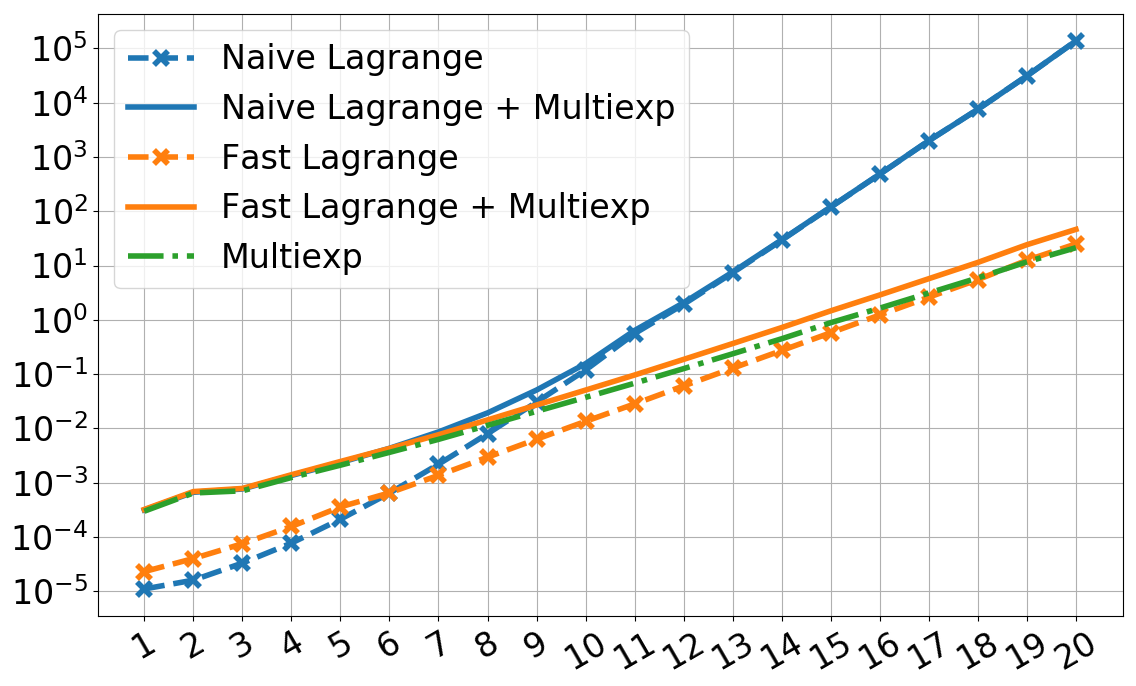
\includegraphics[width=0.33\linewidth]{figures/thresh.png}}
    }
    \subfloat[VSS \& DKG deal time]{\label{f:all-deal-times}%
        {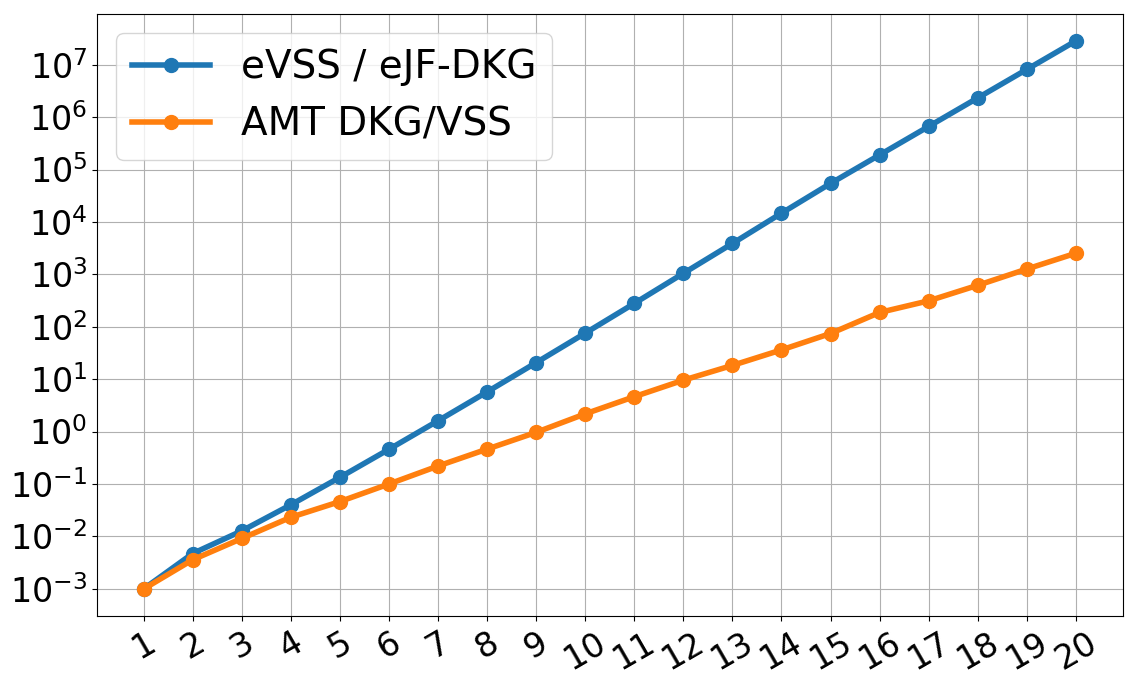
\includegraphics[width=0.33\linewidth]{figures/all-deal-times.png}}
    }
    \subfloat[DKG dealing communication (per player)]{\label{f:dkg-bw}
        {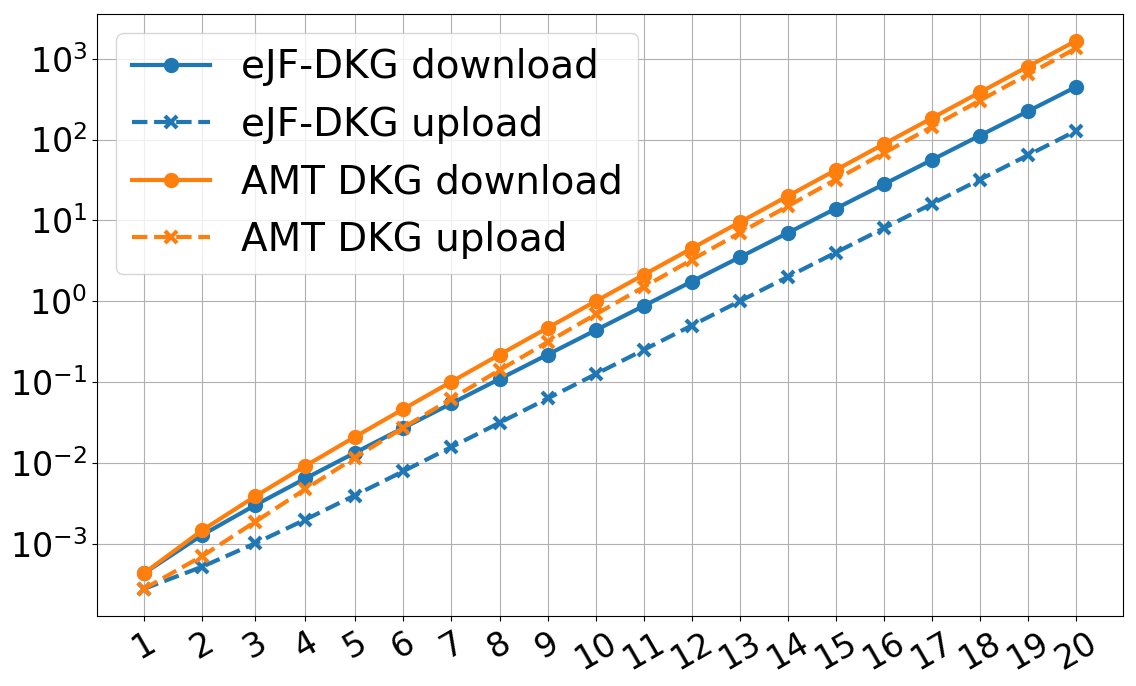
\includegraphics[width=0.33\linewidth]{figures/bw.png}}
    }
    \\
    \subfloat[VSS verify time (per-player)]{\label{f:vss-verify-times}%
        {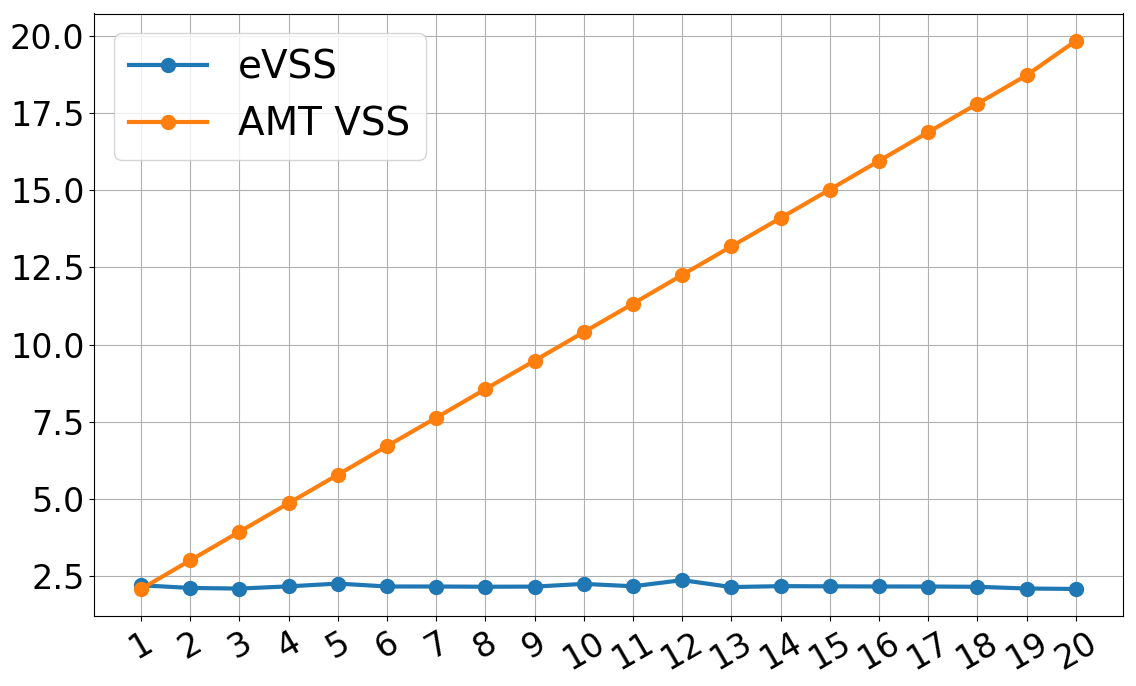
\includegraphics[width=0.33\linewidth]{figures/vss-verify-times.png}}
    }
    \subfloat[VSS reconstruction time]{\label{f:vss-reconstr-times}%
        {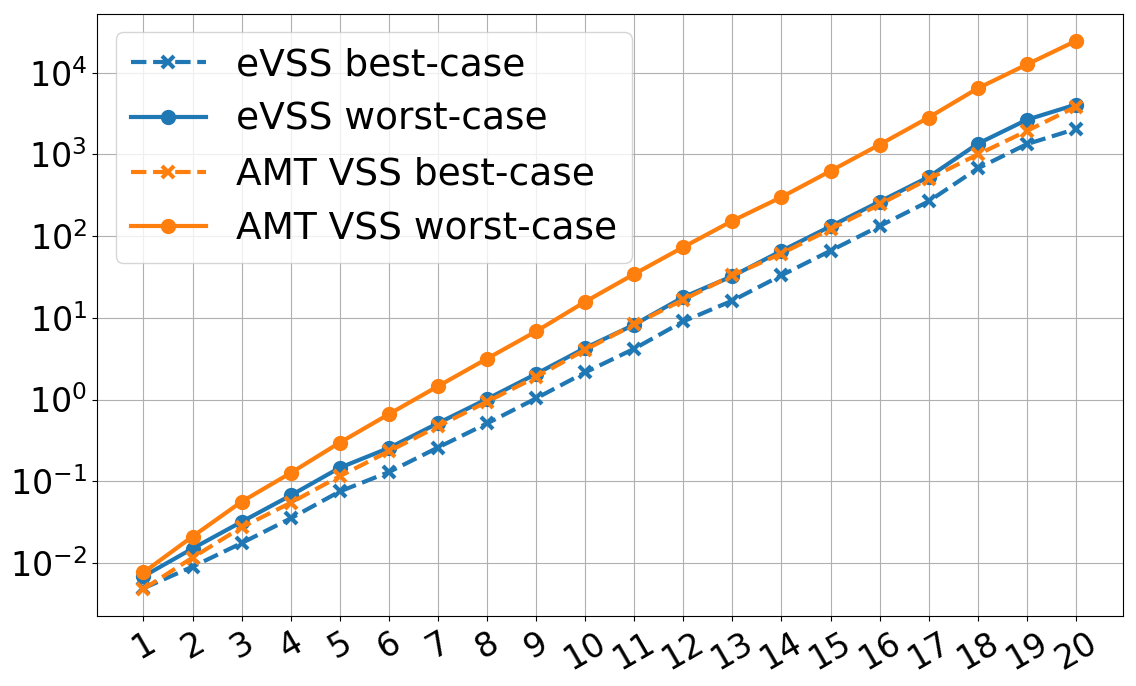
\includegraphics[width=0.33\linewidth]{figures/vss-reconstr-times.png}}
    }
    \subfloat[VSS end-to-end time]{\label{f:vss-e2e-times}%
        {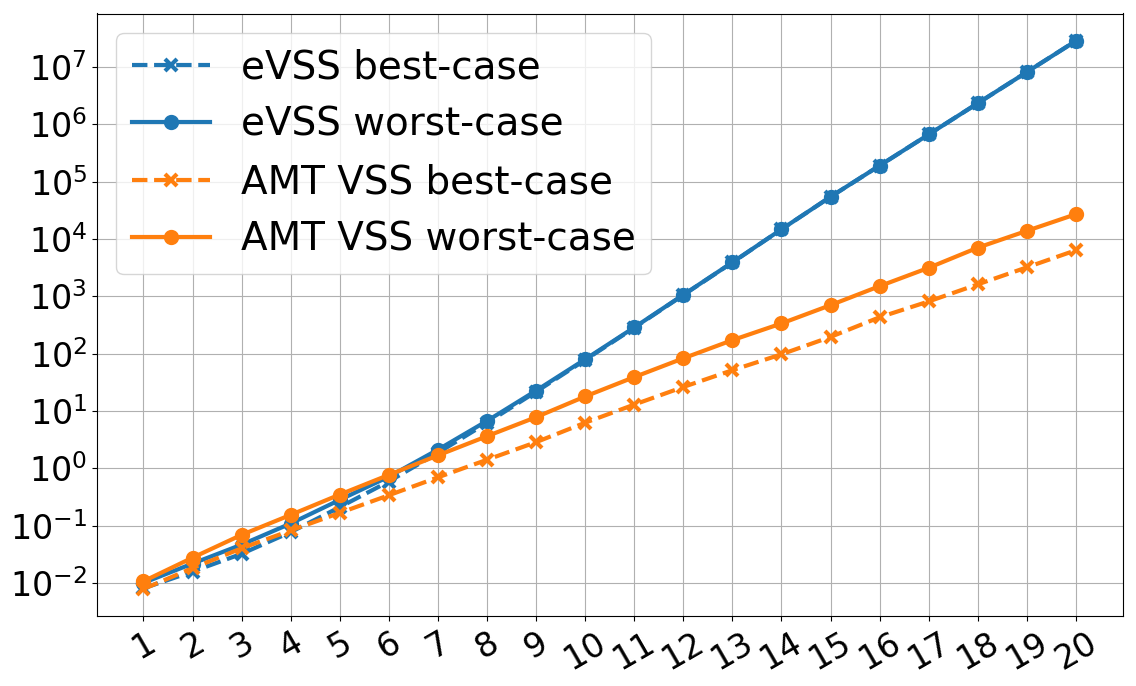
\includegraphics[width=0.33\linewidth]{figures/vss-e2e-times.png}}
    }
    \\
    \subfloat[DKG verify time (per-player)]{\label{f:dkg-verify-times}%
        {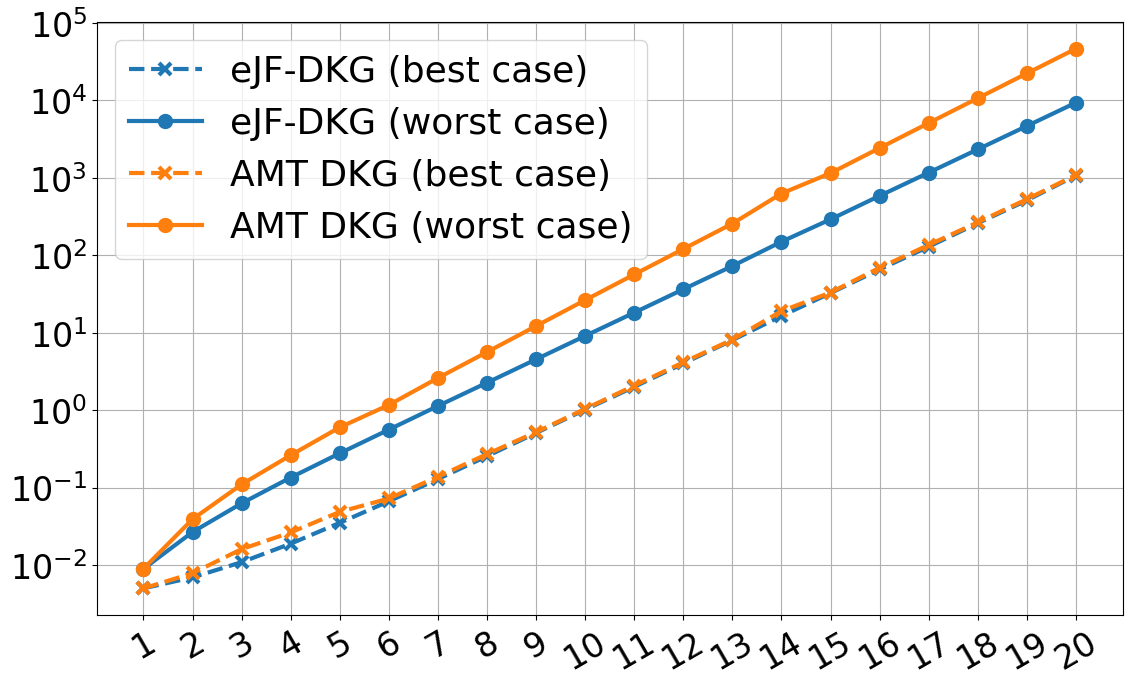
\includegraphics[width=0.33\linewidth]{figures/dkg-verify-times.png}}
    }
    \subfloat[DKG reconstruction time]{\label{f:dkg-reconstr-times}%
        {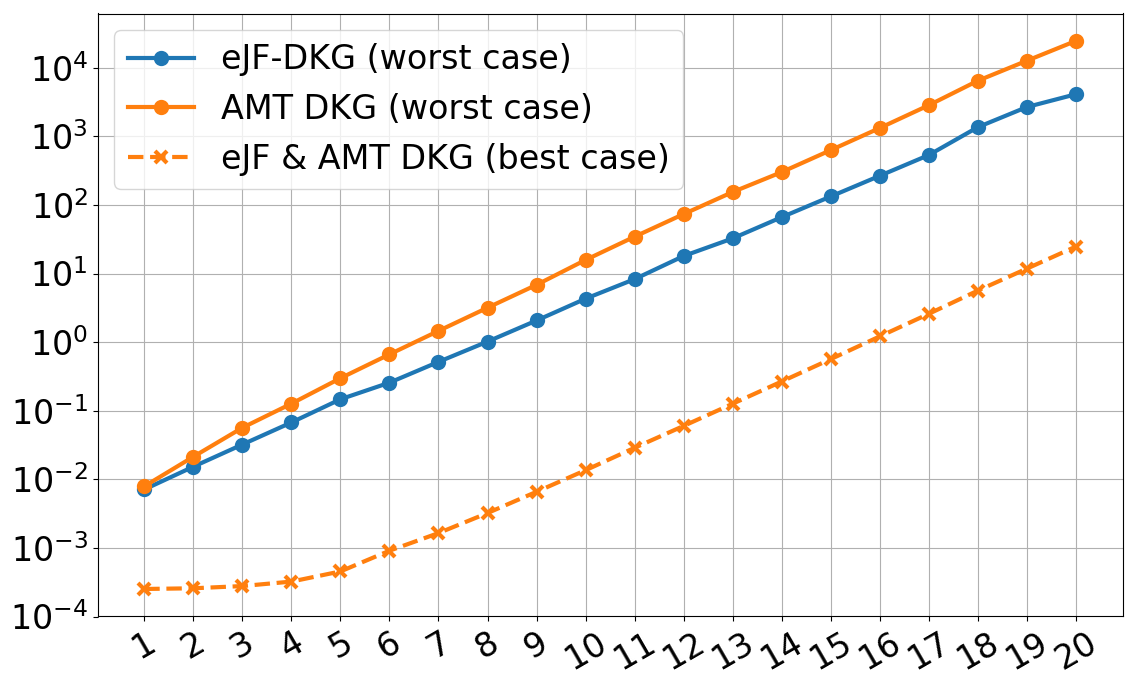
\includegraphics[width=0.33\linewidth]{figures/dkg-reconstr-times.png}}
    }
    \subfloat[DKG end-to-end time]{\label{f:dkg-e2e-times}%
        {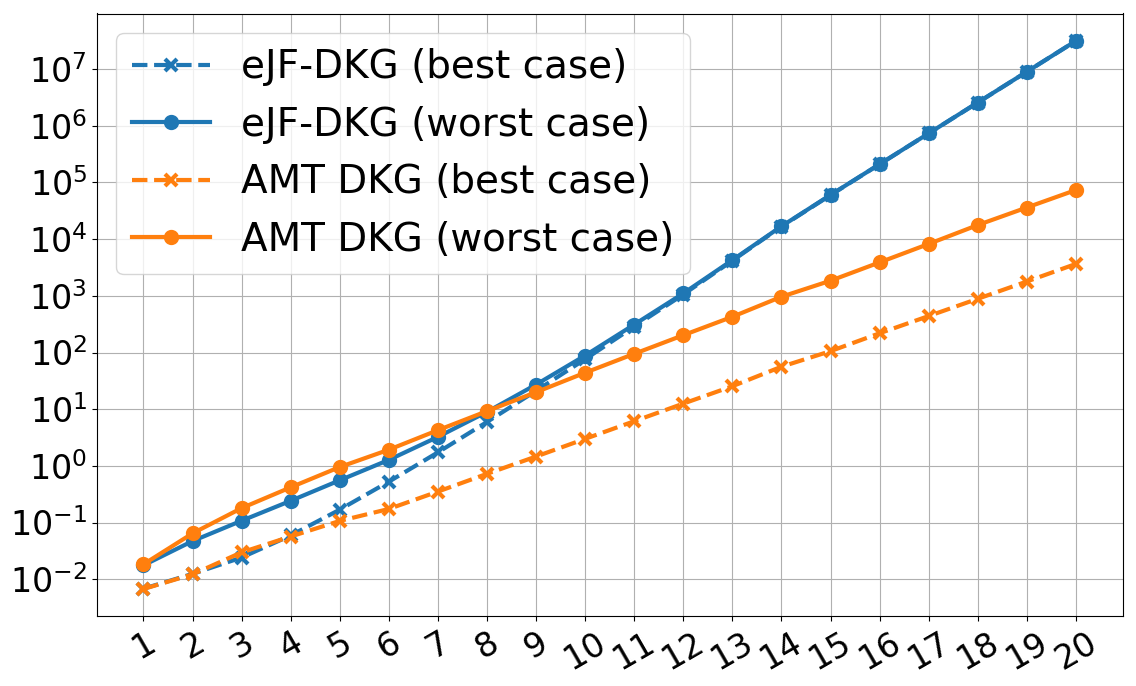
\includegraphics[width=0.33\linewidth]{figures/dkg-e2e-times.png}}
    }
    \caption{
        All benchmarked threshold cryptosystems have threshold $t = f+1$ out of $n=2f+1$.
        %The $x$-axis always indicates the number of players $n$.
        The $x$-axis always indicates $\log_2{t}$.
        The $y$-axis is in seconds, except in \cref{f:dkg-bw} it is in MB and in \cref{f:vss-verify-times} it is in milliseconds.
    }
\end{figure*}

\section{Evaluation}
\label{s:eval}

In this section, we demonstrate the scalability of our proposed cryptosystems.
Our experiments focus on the difficult case when $t > n/2$, specifically $t=f+1$ and $n=2f+1$.
We benchmark TSS, VSS and DKG cryptosystems for thresholds $t \in\{2^1,2^2,2^3,\dots,2^{20}\}$.
Although we did not benchmark other thresholds, similar performance gains would have been observed for other sufficiently large values of $t$ (e.g., $t=f+1$ and $n=3f+1$).
However, we acknowledge that, for sufficiently small $t$, \evss's and \ejfdkg's $\Theta(nt)$ dealing would outperform ours.
Similarly, in this small $t$ setting, naive Lagrange interpolation would outperform fast Lagrange.
Our experiments show that:
\begin{itemize}
    \item Our BLS TSS scales to $n \approx 2$ million signers and outperforms the naive scheme as early as $n=\blsOutperformN$ (see \cref{f:thresh}).
    % Note: Outperforming in the 'worst case'
    \item \ourvss scales to hundreds of thousands of participants, and outperforms \evss as early as $n=\vssOutperformWcN$ (see \cref{f:vss-e2e-times}).
    \item \ourdkg scales to $n\approx$ 65,000 players and outperforms \ejfdkg at $n=\dkgOutperformWcN$ (see \cref{f:dkg-e2e-times}).
\end{itemize}
Importantly, our VSS and DKG speed-ups come at the price of a modest increase in communication (see \cref{f:dkg-bw}).
For example, for $n\approx$ 65,000, a DKG player's communication during dealing increases by \amtDkgCommOverhead{65535} from \ejfDkgComm{65535} in \ejfdkg to \amtDkgComm{65535} in \ourdkg.
However, since the worst-case end-to-end time decreases by \amtDkgEndToEndWcTimeImprovOverejf{65535} from \ejfDkgEndToEndWcTime{65535} in \ejfdkg to \amtDkgEndToEndWcTime{65535} in \ourdkg, the extra communication should be worth it in many applications.

For prohibitively-slow experiments with large $t$, we repeat them fewer times than experiments with smaller $t$.
For brevity, we specify the amount of times we repeat an experiment for each threshold via a \textit{measurement configuration}.
For example, the measurement configuration of our efficient BLS threshold scheme is $\langle 7 \times 100, 13 \times 10 \rangle$.
This means that for the first 7 thresholds $t\in\{2^1,2^2,\dots,2^7\}$ we ran the experiment 100 times while for the last 13 thresholds we ran it 10 times.

\subsubsection{Codebase and experimental setup}
We implemented (1) our BLS threshold signature scheme from \cref{s:threshsig}, (2) \ejfdkg~\cite{Kate2010Distributed} and \ourdkg and (3) \evss~\cite{polycommit} and \ourvss in 5700 lines of C++.
We used a 254-bit Barretto-Naehrig curve with a Type~III pairing~\cite{bn-curve} from Zcash's \texttt{libff}~\cite{libff} elliptic curve library.
We used \texttt{libfqfft}~\cite{libfqfft} to multiply polynomials fast using FFT.
All experiments were run on an Intel Core i7 CPU 980X @ 3.33GHz with 12 cores and 20 GB of RAM, running Ubuntu 16.04.6 LTS (64-bit version).
Since all benchmarked schemes would benefit equally from multi-threading, we did not implement it.

\subsubsection{Limitations}
\label{s:eval:limitations}
Our DKG and VSS evaluations do not account for network delays.
This is an important limitation.
Our focus was on the computational bottlenecks of these protocols.
Nonetheless, scaling and evaluating the broadcast channel of VSS and DKG protocols is necessary, interesting future work.
In particular, ideas from scalable consensus protocols~\cite{algorand} could be used for this.
Finally, our VSS and DKG ``worst case'' evaluations do not fully account for malicious behavior.
Specifically, they do not account for the additional communication and computational cost associated with complaint broadcasting.
We leave this to future work (see \cref{s:sortitioned-dkg}).

\subsection{BLS Threshold Signature Experiments}
\label{s:eval:threshsig}
First, we sample a random subset of $t$ signers $T$ with valid signature shares $\{\sigma_i\}_{i\in T}$.
Second, we compute Lagrange coefficients $\Ell_i^T(0)$ w.r.t. points $x_i = \omega_N^{i-1}$ (see \cref{s:prelim:fft}) using both fast and naive Lagrange.
Third, we compute the final threshold signature $\sigma = \prod_{i\in T} \sigma_i^{\Ell_i^T(0)}$ using a multi-exponentiation.
The measurement configuration for fast Lagrange is $\langle 7 \times 100, 13 \times 10 \rangle$ while for naive Lagrange is $\langle 8\times 100, 6 \times 10, 8, 4, 2, 1,1,1\rangle$.
We plot the average aggregation time in \cref{f:thresh} and observe that our scheme beats the naive scheme as early as $n = \blsOutperformN$.
We do not measure the time to identify valid signature shares via batch verification~\cite{Boldyreva2003Threshold}, which our techniques leaves unchanged.

Our results show that our fast Lagrange interpolation drastically reduces the time to aggregate when $t\approx n/2$.
Specifically, for $n\approx 2^{21}$, we aggregate a signature in \blsEffTime{2097151}, instead of \blsNaiveTime{2097151} if aggregated via naive Lagrange (\blsTimeImprov{2097151} faster).
The benefits are not as drastic for smaller thresholds, but remain significant.
For example, for $n\approx 2^{15}$, we reduce the time by \blsTimeImprov{32767} from \blsNaiveTime{32767} to \blsEffTime{32767}.
For $n=4095$, we see a \blsTimeImprov{4095} speed-up from \blsNaiveTime{4095} to \blsEffTime{4095}.
For $n=2047$, we see a \blsTimeImprov{2047} speed-up from \blsNaiveTime{2047} to \blsEffTime{2047}.

\subsection{Verifiable Secret Sharing Experiments}
\label{s:eval:vss}
% Note: VSS plots resemble DKG plots
%  VSS deal       ~= DKG per-player deal
%   - but DKG additionally computes f_i(0) proof and NIZKPoK
%  VSS verify     != DKG per-player verify / (n-1)
%   - because DKG also verifies f_i(0) which adds extra work
In this section, we benchmark \evss and \ourvss.
We do not benchmark the complaint round since, when implemented with KZG batch proofs, it remains the same (see \cref{s:scalable-vss:batch-complaints}).
% We do not benchmark Feldman's VSS because it has a larger $\Theta(t)$-sized broadcast.

\subsubsection{VSS dealing}
\label{s:eval:vss:deal}
For \evss dealing, the measurement configuration is $\langle 10 \times 10, 3, 2, 2, 1, 1, 0, 0, 0, 0, 0\rangle$.
For large $t\ge 2^{16}$, \evss dealing is too slow, so we extrapolate it from the previous dealing time (i.e., we multiply by 3.5).
For \ourvss dealing, the measurement configuration is $\langle12 \times 100, 50, 22, 10, 5, 3, 2, 1, 1\rangle$.
In \evss, we compute the shares $s_i$ ``for free'' as remainders of the $\phi(x) / (x-i)$ divisions.
We plot the average dealing time in \ourvss and \evss as a function of $n$ in \cref{f:all-deal-times}.
Our results show that \ourvss's \amtDealTime dealing scales much better than \evss's $\Theta(nt)$ dealing.
For example, for $n\approx 65,000$, \evss takes \evssVssDealTime{65535} while \ourvss takes \amtVssDealTime{65535}.
For very large $n\approx 2^{21}$, \evss takes a prohibitive \evssVssDealTime{2097151} while \ourvss takes \amtVssDealTime{2097151}.
We find that \ourvss's dealing outperforms \evss's as early as $n=\amtVssDealTimeOutperformNevss$.

\subsubsection{VSS verification round}
\label{s:eval:vss:share-verif}
In \cref{f:vss-verify-times}, we plot the time for one player to verify its share.
The measurement configuration is $\langle 20 \times 1000\rangle$ for both schemes.
In \evss, verification requires two pairings and one exponentiation in $\Group_1$, taking on average $2.15$ ms.
In \ourvss, verification requires $\amtProofSize{t}$ pairings and one exponentiation in $\Group_1$, ranging from \amtVssVerifyTime{3} ($n=3$) to \amtVssVerifyTime{2097151} ($n\approx 2^{21}$).

\subsubsection{VSS reconstruction}
\label{s:eval:vss:reconstr}
In \cref{f:vss-reconstr-times}, we plot the time to reconstruct the secret.
We consider the \textit{best-case} and \textit{worst-case} times, as detailed in \cref{s:scalable-vss:reconstruction}.
For \evss, ``best case'' means the first $t$ share verifications are successful and ``worst case'' means the first $n-t$ are unsuccessful (see \cref{s:scalable-vss:reconstruction}).
The measurement configuration is $\langle 5 \times 1000, 500, 250, 120, 60, 30, 15, 5\times 10, 8,4,2,1\rangle$ for \evss and $\langle 9 \times 100, 4\times 10, 4,2, 5\times 1\rangle$ for \ourvss.
In both protocols, the (fast) Lagrange interpolation time is insignificant compared to the time to verify shares during reconstruction (e.g., for $n\approx 2^{21}$ in \evss, interpolation is only \fastLagrTime{2097151} out of the total \evssVssReconstrBcTime{2097151} worst-case time).

\ourvss's best-case is very close to \evss's worst-case.
This is because, with the help of memoization, \ourvss's best case only computes $\le 2n-1$ pairings (i.e., the number of nodes in a full binary tree with $n$ leaves).
This closely matches the $2n$ pairings in \evss's worst case.
(In practice, we replace $n$ of these pairings and $\Group_1$ exponentiations by $n$ $\Group_T$ exponentiations, which are slightly faster.)
\ourvss's worst case is \evssVssReconstrWcTimeImprovOveramt{3} to \evssVssReconstrWcTimeImprovOveramt{2097151} slower than \evss's.
But we show next that our faster dealing more than makes up for this.
Finally, \evss's best-case time is half its worst-case time, as expected.

% The worst ordering is to first naively verify the $n-t$ invalid shares in $\Theta((n-t)\log{t})$ time and then verify the remaining $t$ valid shares efficiently using memoization in $\Theta(t)$ time.
%Our experiments simulate exactly this case.
%Our experiments use fast Lagrange interpolation from \cref{f:thresh}.

\subsubsection{VSS end-to-end time}
\label{s:eval:vss:end-to-end}
Finally, we consider the \textit{end-to-end time}, which is the sum of the sharing and reconstruction phase times.
(Again, a limitation of our work is ignoring the overhead of the complaint round in the worst case.)
\cref{f:vss-e2e-times} gives the best- and worst-case end-to-end times.
The key takeaway is that \ourvss's smaller dealing time makes up for the increase in its verification round and reconstruction phase times.
\ourvss outperforms \evss's worst-case time at $n\ge \vssOutperformWcN$ and its best-case time at $n\ge \vssOutperformBcN$.
For example, for large $n=16,383$, we reduce the worst-case time from \evssVssEndToEndWcTime{16383} to \amtVssEndToEndWcTime{16383} and the best-case time from \evssVssEndToEndBcTime{16383} to \amtVssEndToEndBcTime{16383}.
The best case improvement ranges from \amtVssEndToEndBcTimeImprovOverevss{\vssOutperformBcN} ($n=\vssOutperformBcN$) to \amtVssEndToEndBcTimeImprovOverevss{2097151} ($n\approx 2^{21}$).
The worst case improvement ranges from \amtVssEndToEndWcTimeImprovOverevss{\vssOutperformWcN} ($n=\vssOutperformWcN$) to \amtVssEndToEndWcTimeImprovOverevss{2097151} ($n\approx 2^{21}$).
Thus, we conclude \ourvss scales better than \evss.

\subsection{Distributed Key Generation Experiments}
\label{s:eval:dkg}

Our DKG experiments mostly tell the same story as our VSS experiments:
AMTs drastically reduce the dealing time of DKG players, which more than makes up for the slight increase in verification and reconstruction time.
However, \ourdkg has a \amtDkgCommOverhead{7} to \amtDkgCommOverhead{2097151} communication overhead during dealing.
Still, we believe this is worth the drastic reduction in end-to-end times (see \cref{s:eval:dkg:e2e-time}).

\subsubsection{DKG dealing}
DKG dealing time is equal to VSS dealing time (see \cref{s:eval:vss:deal}) plus the time to compute a KZG proof and a NIZKPoK for $g^{f_i(0)}$.
However, as $n$ increases, the time to compute these two proofs pales in comparison to the time to compute the $n$ evaluation proofs.
Thus, in \cref{f:all-deal-times}, we treat DKG dealing times as equal to VSS dealing times.
%(Indeed, separate VSS and DKG lines in \cref{f:all-deal-times} would be hard to distinguish.)
As a result, the same observations apply here as in \cref{s:eval:vss:deal}: AMTs drastically reduce dealing times.

\subsubsection{DKG verification round}
\label{s:eval:dkg:share-verif}
We consider both the \textit{best case} and the \textit{worst case} verification time, as discussed in \cref{s:scalable-dkg:share-verif}.
In our best-case experiment, each player $j$ aggregates all its shares as $s_j=\sum_{i\in[n]} s_{i,j}$ and their evaluation proofs as $\pi_j$.
Then, $j$ verifies $s_j$ against $\pi_j$.
Similarly, $j$ aggregates and efficiently verifies all its $g^{f_i(0)}$'s and their KZG proofs.
In the worst-case experiment, $j$ individually verifies the $s_{i,j}$ shares and the $g^{f_i(0)}$'s.
Importantly, in both experiments, $j$ individually verifies all $n$ NIZKPoKs for $g^{f_i(0)}$ in $\Theta(n)$ time.
The two experiments are meant to bound the time of a realistic implementation that carefully uses \textit{batch verification}~\cite{Boldyreva2003Threshold,LM07} to not exceed the worst-case time too much.

The best-case \ejfdkg measurement configuration is $\langle 8 \times 100, 50, 25, 12, 9 \times 10\rangle$ and the worst-case is $\langle 5 \times 100, 50, 25, 12, 12\times 10 \rangle$.
For \ourdkg, the best-case configuration is $\langle 12\times 100, 80, 40, 20, 16, 8, 4, 3, 2 \rangle$ and the worst-case is $\langle 5 \times 100, 4\times 80, 40, 20, 8, 4, 2, 6\times 1 \rangle$.
The average per-player verification times are plotted in \cref{f:dkg-verify-times}.
In the best case, both schemes perform roughly the same, since the verification of the $n$ NIZKPoKs quickly starts dominating the aggregated proof verification.
In the worst case, \ourdkg time ranges from \amtDkgVerifyWcTime{3} ($n=3$) to \amtDkgVerifyWcTime{2097151} ($n \approx 2^{21}$).
In contrast, \ejfdkg time ranges from \ejfDkgVerifyWcTime{3} to \ejfDkgVerifyWcTime{2097151} (\ejfDkgVerifyWcTimeImprovOveramt{7} to \ejfDkgVerifyWcTimeImprovOveramt{2097151} faster).
Nonetheless, \ejfdkg remains slower overall due to its much slower dealing (see \cref{s:eval:dkg:e2e-time}).
Both best- and worst-case times can be reduced by batch-verifying NIZKPoKs, which resemble Schnorr signatures~\cite{Schnorr89} and are amenable to batching~\cite{BDL+12}.

\subsubsection{DKG reconstruction}
\label{s:eval:dkg:reconstr}
Here the measurement configuration is $\langle 4\times 1000, 200, 50, 25, 13\times 10\rangle$ and times are plotted in \cref{f:dkg-reconstr-times}.
The best case is very fast in both \ejfdkg and \ourdkg, taking only \amtDkgReconstrBcTime{2097151} for $t=2^{20}$, since both schemes interpolate the secret $s$ without verifying shares and check it against $g^s$ (see \cref{s:scalable-dkg:reconstr}).
For the worst case, the time is the sum of (1) the (failed) best-case reconstruction time and (2) the worst-case time to identify $t$ valid shares from $n$ shares.
Since the best case is very fast, the DKG worst-case time (see \cref{f:dkg-reconstr-times}) looks almost identical to its VSS counterpart (see \cref{f:vss-reconstr-times}).
Note that the same \ourvss speed-up techniques for finding $t$ valid shares apply in \ourdkg (see \cref{s:scalable-vss:reconstruction}).
\ourdkg's worst case is anywhere from \ejfDkgReconstrWcTimeImprovOveramt{3} to \ejfDkgReconstrWcTimeImprovOveramt{2097151} slower than \ejfdkg's, much like \ourvss.
However, as we show next, \ourdkg's faster dealing more than makes up for this.

\subsubsection{DKG end-to-end time}
\label{s:eval:dkg:e2e-time}

Similar to the VSS experiments in \cref{s:eval:vss:end-to-end}, we consider the \textit{end-to-end time}.
\cref{f:dkg-e2e-times} plots the best- and worst-case end-to-end times and shows that \ourdkg outperforms \ejfdkg starting at $n\ge \dkgOutperformBcN$ (in the best case) and at $n\ge\dkgOutperformWcN$ (in the worst case).
This is a direct consequence of \ourvss outperforming \evss, since the DKG protocols use these VSS protocols internally.
For example, for large $n=16,383$, we reduce the worst-case end-to-end time from \ejfDkgEndToEndWcTime{16383} to \amtDkgEndToEndWcTime{16383} and the best-case time from \ejfDkgEndToEndBcTime{16383} to \amtDkgEndToEndBcTime{16383}.
The improvement in best-case end-to-end time ranges from \amtDkgEndToEndBcTimeImprovOverejf{\dkgOutperformBcN} ($n=\dkgOutperformBcN$) to \amtDkgEndToEndBcTimeImprovOverejf{2097151} $(n\approx2^{21})$ and, in the worst case, from \amtDkgEndToEndWcTimeImprovOverejf{\dkgOutperformWcN} to \amtDkgEndToEndWcTimeImprovOverejf{2097151}.
Thus, we conclude \ourdkg scales better than \ejfdkg.

\subsubsection{DKG communication}
\label{s:eval:dkg:communication}

We estimate each player's upload and download during the dealing round.
For upload, each \ejfdkg and \ourdkg player $i$ has to broadcast a KZG commitment $g^{f_i(\tau)}$ (32 bytes) and a commitment $g^{f_i(0)}$ with a NIZKPoK and a KZG proof (32 + 64 + 32 bytes).
Then, $i$ has to send each $j\in[n]$ its share (32 bytes) with an evaluation proof (32 bytes for KZG or $(\amtProofSize{t}) \cdot 32$ bytes for AMT).
For download, each player $i$, has to download $n-1$ shares, each with their KZG commitment and evaluation proof, plus $n-1$ $g^{f_j(0)}$'s, each with their NIZKPoK and KZG proof.
Note that \ourdkg uses KZG proofs for $g^{f_i(0)}$ to minimize its communication overhead.

We plot the upload and download numbers for both schemes in \cref{f:dkg-bw}.
\ejfdkg's per-player upload ranges from \ejfDkgUpload{3} to \ejfDkgUpload{2097151} while download ranges from \ejfDkgDownload{3} to \ejfDkgDownload{2097151}.
\ourvss's upload overhead ranges from \amtDkgUploadOverhead{3} to \amtDkgUploadOverhead{2097151} and its download overhead ranges from \amtDkgDownloadOverhead{3} to \amtDkgDownloadOverhead{2097151}.
Overall, \ourvss's upload-and-download overhead ranges from \amtDkgCommOverhead{3} to \amtDkgCommOverhead{2097151}.
Thus, we believe the \amtDkgEndToEndBcTimeImprovOverejf{2097151} and \amtDkgEndToEndWcTimeImprovOverejf{2097151} reductions in best- and worst-case end-to-end times are sufficiently large to make up for this overhead.
  \section{Discussion and Future Work}
\label{s:discussion}

\subsubsection{Generating public parameters}
\label{s:trusted-setup}
% Note: Using a DKG for the trusted setup could be problematic because of attacks on f+1 out of 2f+1 DKGs where f malicious players complain about f honest players, forcing them to reveal their secrets, resulting in just only one (albeit honest) player knowing the secret (and everybody else knowing that the honest player knows, and therefore possibly targetting him).
Similar to \evss and \ejfdkg, our protocols require a \textit{trusted setup} to generate $\ell$-SDH public parameters.
Fortunately, this setup needs to be done only once and can be securely implemented via MPC protocols~\cite{zcash-mpc1,zcash-mpc2}.
In fact, currently deployed systems have already demonstrated the practicality of this approach.
In 2018, approximately 200 participants used an MPC~\cite{zcash-mpc2} to generate new public parameters for the Sapling version of Zcash~\cite{zcash}.
The MPC protocol allowed anyone to participate and only required one honest party, making it a very good candidate.

\subsubsection{Sortitioned DKG}
\label{s:sortitioned-dkg}
To further reduce communication and computation, we propose a \textit{sortitioned DKG} where only a small, random \textit{committee} of $c < n$ players deal.
The key question is where does the randomness to pick the committee come from?
When a DKG runs many times, this randomness could come from previous DKG runs (e.g., DKGs for Schnorr TSS nonces).
To bootstrap securely, the first DKG run would be with a full committee of size $c=n$.
When a DKG runs only once, such as when distributing the secret key of a $(t,n)$ TSS, the $c$ players could be a decentralized cothority~\cite{cosi} different than the TSS signers.
The cothority would run the DKG dealing round while the $n$ signers would run the DKG verification round (see \cref{alg:dkg}).
The complaint round would be split: accused cothority members would compute the KZG batch proofs (see \cref{s:scalable-vss:batch-complaints}) while the $n$ signers would receive and verify those proofs.
Importantly, our AMT technique would help cothority members deal much faster to the $n$ signers.
We leave defining and proving the security of sortitioned DKGs to future work.

\subsubsection{Arbitrary points}
\label{s:amt:arbitrary-points}
AMTs can be generalized to any set of points $\{x_i\}_{i\in[n]}$ (not just $x_i=\omega_N^{i-1}$) \textit{for which verifiers do not have the necessary accumulator commitments}.
The accumulators $g^{a_{w}(\tau)}$ can be included as part of the proof \textit{but} along with (1) a subset proof w.r.t. the parent accumulator and (2) an ``extractable'' counterpart $g^{\alpha a_w(\tau)}$, where $\alpha$ is another trapdoor.
% Note: Need to add: 
% - 64 byte accumulator in G2 (so we can pair it with G1 quotient), 
% - 32 bytes for extractable counterpart in G1 (so we can check it for equality against accumulator in G2 and g^\tau in G1)
% - 32 bytes for the subset proof in G1 (so we can pair with child accumulator in G1).
% So overhead goes from 32 bytes per node to 128 bytes per node.
The asymptotic proof size remains the same but will increase in practice by 4x (with Type III pairings).
Furthermore, this construction will need extra public parameters of the form $(g^{\alpha \tau^i})_{i\in[0,\ell]}$.
On the other hand, proof verifiers now need $\Theta(1)$ rather than $\Theta(\log{n})$ public parameters (see \cref{s:amt:public-parameters,s:scalable-vss:public-params}).
We leave proving this construction secure under $\ell$-PKE~\cite{groth10} to future work.

\subsubsection{Information-theoretic hiding AMTs}
\label{s:amt:information-theoretic-amts}
We can devise an information-theoretic hiding version of our AMT proofs that is compatible with information-theoretic hiding KZG commitments~\cite{polycommit}.
This version of AMTs can be used to speed up the unbiasable \newdkg protocol~\cite{dkg}. 
%, although other ways of getting unbiasability exist~\cite{NBB16}.
% Our evaluation focused on the biasable protocols since we would have observed an improvement of roughly the same magnitude in the unbiasable protocols too.
% Also for simplicity of presentation, since the PK $\sum_i g^{z_i}$ can be extracted in a simple way.
Let $h=g^{\kappa}$ be another generator of $\Group$ such that nobody knows the discrete log $\kappa=\log_g(h)$.
Assume that, in addition to $\mathsf{PP}_q(g; \tau)$, we also have public parameters $\mathsf{PP}_\ell(h;\tau)$.
An information-theoretic hiding KZG commitment to $\phi$ of degree $d$ is $c = g^{\phi(\tau)} h^{r(\tau)} = g^{\phi(\tau)+\kappa r(\tau)}$ where $r$ is a random, degree $d$ polynomial~\cite{polycommit}.
Note that $c$ is just a commitment to the polynomial $\psi(x) = \phi(x) + \kappa r(x)$.
As a consequence, all we have to do is build an AMT for $\psi$.
For this, we compute an AMT for $\phi$ with public parameters $\PP_\ell(g;\tau)$ and one for $r$ but with parameters $\PP_\ell(h;\tau)$.
By homomorphically combining these two AMTs we get exactly the AMT for $\psi$ (see \cref{s:scalable-dkg:homomorphic-amt}).
We leave proving this construction is information-theoretic hiding to future work.
% Note that the 'hiding' definition from the KZG paper gives the adversary the commitment and a bunch of evaluation proofs, so as to account for the fact that proofs might reveal the polynomial.

\subsubsection{Vector commitments (VCs)}
AMTs naturally give rise to a VC scheme with logarithmic-sized proofs~\cite{vc}.
Similar to the multivariate polynomial-based VC from~\cite{edrax}, this scheme would also support efficiently updating proofs and updating VC digests after vector updates.
Thus, our VC could also be used for building stateless cryptocurrencies~\cite{edrax,BBF19}.
Our VC can be extended with zero-knowledge-like properties using the information-theoretic variant of AMTs (see \cref{s:amt:information-theoretic-amts}).

\subsubsection{Batch AMT verification}
\label{s:amt:batch-verification}
The efficient reconstruction techniques from \cref{s:scalable-vss:reconstruction} reduced the number of pairings when verifying an AMT, but still required $\Theta(t + (n-t)\log{t})$ pairings in the worst case.
At the cost of doubling the prover time and proof size, this can be reduced to $\approx 2n-1$ pairings, independent of how many proofs are valid.
The key idea is to also include commitments to the \textit{remainder polynomials} from the multipoint evaluation tree in the AMT (see \cref{f:multipoint-eval}).
This way, an entire AMT tree can be verified node-by-node, top-to-bottom by checking that the division at each node is correct.
We leave proving this approach secure to future work.

  \section{Conclusion}

We introduced new techniques that both speed up and scale threshold cryptosystems.
First, we showed how computing Lagrange coefficients efficiently can drastically reduce threshold signature aggregation time.
We believe our fast BLS threshold signature scheme can be used to design simple, large-scale, decentralized random beacons.
Second, we introduced a quasilinear time technique for precomputing proofs in KZG polynomial commitments.
When applied to VSS and DKG protocols, this technique drastically reduces computation without increasing communication too much.
We left scaling the broadcast channel and the complaint round to future work.

  \clearpage
  %\nocite{*}
  \bibliographystyle{IEEEtran}
  \bibliography{references} 
  
  %\clearpage
  \appendix
  \subsection{AMT Prover Time and Proof Sizes}
\label{s:amt:proof-time-and-sizes}
We will restrict ourselves to our $n = 2^m$ and $\deg{\phi}=t-1 < n$ setting.
We first show that computing our optimized, roots-of-unity-based AMT takes $O(n\log{t})$ time (see \cref{s:amt:roots-of-unity}).
The key observation is that, when computing the AMT, divisions at higher levels (i.e., closer to the root) in the tree are \textit{trivial} and need not be performed.
Specifically, at sufficiently high levels, the degree of the divisors (i.e., accumulators) are larger than the degrees of the dividends (i.e., remainders), and always give quotients equal to zero.
Since zero quotients can be easily recreated by verifiers, their commitments need not be included in the proof.
We expand on this next.

Let us number levels differently, from $\log{n}$ (the root) to 0 (the leaves), so that level $i$ has $n/2^i$ nodes, each with an accumulator of degree $2^i$.
Now, let $k$ be the smallest value such that $2^k \le \deg{\phi} < 2^{k+1}$.
In other words, $k$ is the level at which accumulator degrees are $\le \deg{\phi}$ and thus divisions are non-trivial.
Put differently, each node on level $k$ will be the root node of an (authenticated) multipoint evaluation (sub)tree.
We argue that the time to compute any one such subtree is $O(2^k \log{2^k})$ and, since there are $n/2^k$ such subtrees, the final AMT takes $O(n\log{2^k}) = O(n\log{t})$ time since $2^k\le t-1=\deg{\phi}$.
We prove this inductively next.

At the root node of a level $k$ subtree, the dividend $d_k = \phi$ has $\deg{d_k} < 2^{k+1}$ (by definition of $k$ above).
The accumulator $a_k$ has $\deg{a_k} = 2^k$.
Thus, the quotient $q_k = d_k/a_k$ will have $\deg{q_k} = \deg{d_k}-\deg{a_k}< 2^{k+1} - 2^k = 2^k$ and the remainder $r_k = d_k \bmod a_k$ will have $\deg{r_k} < \deg{a_k} = 2^k$.
The division at this level will only take $O(\deg{d_k})=O(2^{k+1})$ time, thanks to the $(x^{2^k} + c)$ form of $a_k$.
Committing to the quotient will take $O(2^{k})$ time.
To summarize, at level $k$ we are doing $O(2^{k+1})$ work and $\deg{d_k} < 2^{k+1}, \deg{a_k} = 2^k, \deg{q_k} < 2^k, \deg{r_k} < 2^k$.
Next, we argue that the amount of work \textit{per node} on level $k-1$ is half the work per node at level $k$.
This is because (1) the dividend $d_{k-1}$ is set to the remainder $r_k$ from the parent, so $\deg{d_{k-1}} < 2^k$, (2) $\deg{a_{k-1}}=2^{k-1}$, (3) $\deg{q_{k-1}} = \deg{d_{k-1}}-\deg{a_{k-1}}<2^k-2^{k-1}=2^{k-1}$ and (4) $\deg{r_{k-1}} < \deg{a_{k-1}}=2^{k-1}$.
Thus, at level $k-1$, the division takes $O(2^k)$ time and committing to the quotient takes $O(2^{k-1})$ time. 
As a result, the time to compute the subtree can be expressed as $T(2^{k+1}) = 2T(2^{k+1} / 2) + O(2^{k+1}) = O(2^{k}\log{2^{k}})$.

% - Q: What is proof computation time then? A: $O(n\log{t})$
%    - Let $k$ be the greatest value such that $2^k \le t-1 < 2^{k-1}$.
%    - $k$ is the level where we actually start dividing the root polynomial $p$ of degree $t-1$ by an accumulator of degree $2^k$
%    - At level $k$ (where $k=0$ are the leaves), we have $n/2^k$ nodes.
%    - At each node on level $k$, we do an $O(t)$ division (dividend has deg $t-1$ and divisor has deg less than that)
%    - And, in that node's subtree, we do $O(t\log{t})$ work overall
%    - So, in the whole tree we do $O(n/2^k t\log{t})$ work
%    - So close to $O(n\log{t})$ time

Finally, an AMT proof is $O(\log{t})$-sized.
Recall that quotients in the AMT are non-zero only at levels $k$ and below, where $2^k \le t-1 < 2^{k+1}$.
Thus, an AMT proof will only have non-zero quotients at levels $k, k-1, k-2, \dots, 1, 0$.
Since $k = \floor{\log_2(t-1)}$ the exact proof size is $\floor{\log_2(t-1)}+1$ group elements.

% - Q: Are our proofs $O(\log{t})$ or $O(\log{n})$?
% - A: $\mathsf{floor}(\log_2{(t-1)}) + 1$
%    + We only start dividing by accumulators of deg $< t$
%    - Each time we divide, the next level has an accumulator of deg $t/2$ and a remainder of deg $< t-1$
%    - $\log_2{(t-1)}$ makes sense because the accumulators from the leaves to the roots have degree $1, 2, 4, \dots, n$, at some point reaching a maximum degree $2^k \le t-1 \Leftrightarrow k \le \log_2{(t-1)}$
%       + i.e., $k = \mathsf{floor}(\log_2(t-1))$
%    - The exact proof size should be $k+1$, I think. For example, consider $t-1 = 2$ (or even 3). 
%        - Then, the largest accumulator we'll "successfully" / "usefully" divide by will be deg $2^k = 2^1$. (Larger accumulators will give quotient 0 and remainder equal to the dividend.) 
%        - Dividing by the acc of deg $2^1$ will give a remainder of deg $\le$ 1 and a non-zero quotient.
%        - Another division will be needed at the level below, by an accumulator of deg 1.
%        - Thus, the proof consists of these two quotients.
%        - So its size is $k+1$.
%    - So in the code, the proof size should be $1 + \mathsf{floor}(\log_2(t-1))$

  \subsection{Cryptographic Assumptions}
\label{s:assumptions}

Let $\poly(\cdot)$ denote any function upper-bounded by some univariate polynomial.

\begin{definition}[Bilinear pairing parameters]
\label{d:bilinear-pairing-parameters}
Let $\mathcal{G}(\cdot)$ be a randomized polynomial algorithm with input a security parameter $\lambda$.
% -- begin multiline --
Then, $\langle \Group, \GT, p, g, e\rangle \leftarrow \mathcal{G}(1^\lambda)$ are called \textit{bilinear pairing parameters} if
$\Group$ and $\GT$ are cyclic groups of prime order $p$ where discrete log is hard, 
$\Group$ has generator $g$
and if $e$ is a bilinear map, $e : \Group\times \Group \rightarrow \GT$ such that $\GT = \langle e(g,g) \rangle$.
% -- end multiline --
\end{definition}

\begin{definition}[$\ell$-Strong Bilinear Diffie-Hellman (SBDH) Assumption]
\label{d:q-sbdh}
Given as input security parameter $1^\lambda$, bilinear pairing parameters $\langle \Group, \GT, p, g, e\rangle \leftarrow \mathcal{G}(1^\lambda)$,
public parameters  $\mathsf{PP}_q(g;\tau)=\langle g, g^\tau, g^{\tau^2},\allowbreak \dots, g^{\tau^\ell}\rangle$ where $\ell = \poly(\lambda)$ and $\tau$ is chosen uniformly at random from $\Zp^*$, no probabilistic polynomial-time adversary can output a pair $\langle c, e(g,g)^\frac{1}{\tau+c}\rangle$ for some $c \in \Zp$, except with probability negligible in $\lambda$.
\end{definition}


\begin{definition}[$\ell$-Polynomial Diffie-Hellman (polyDH) Assumption]
\label{d:poly-dh}
Given as input security parameter $1^\lambda$, bilinear pairing parameters $\langle \Group, \GT, p, g, e\rangle \leftarrow \mathcal{G}(1^\lambda)$,
public parameters $\mathsf{PP}_q(g;\tau)=\langle g, g^\tau, g^{\tau^2},\allowbreak \dots, g^{\tau^\ell}\rangle$ where $\ell = \poly(\lambda)$ and $\tau$ chosen uniformly at random from $\Zp^*$, no probabilistic polynomial-time adversary can output $(\phi(x), g^{\phi(\tau)}) \in \Zp[X]\times \Group$, such that $2^\lambda > \deg{\phi} > \ell$, except with probability negligible in $\lambda$.
% Q: Why does KZG condition 2^\lambda > \deg{\phi}? Could a PPT adversary ever output such a polynomial?
% A: I guess it could, depending on the format, because such a polynomial could have lots of zero coefficients which don't need to be outputted.
\end{definition}

\subsection{AMT Proofs are Computationally Hiding and Binding}
\label{s:proofs}
Recall from ~\cite{polycommit} that a polynomial commitment scheme consists of six algorithms: \polysetup, \polycommit, \polyopen, \polyverifypoly, \polycreatewitness, \polyverifyeval.
We show our modified KZG scheme with AMT proofs satisfies \textit{computational hiding} (see \cref{d:polycommit:comp-hiding}) under the discrete log (DL) assumption and \textit{evaluation binding} (see \cref{d:polycommit:eval-binding}) under the $\ell$-Strong Bilinear Diffie-Hellman ($\ell$-SBDH) assumption.
These properties were originally defined in \cite{polycommit}.
We prove these properties hold for a more general scheme that builds AMTs for an arbitrary set $X$ of $n$ points (rather than just for the set of roots of unity).
For this scheme, \polysetup returns not only $\ell$-SDH public parameters, but also the accumulator commitments necessary to verify AMT proofs.
In other words, given an evaluation point $x^{*} \in X$, verifiers have access to accumulators $\{g^{a_w(\tau)}\}_{w\in\treepath(x^{*})}$ necessary to verify $x^{*}$'s AMT proof.
%(Recall that accumulators of degree $>\deg{\phi}$ can be discarded; see \cref{s:amt:public-parameters}.)

%We use Kate et al.'s definition of polynomial commitments~\cite{polycommit}.

%\api \polysetup$(\lambda, \ell)\rightarrow \pp$.
%\api \polycommit$(\pp, \phi)\rightarrow c, d$.
%\api \polyopen$(\pp, c, \phi, d)\rightarrow \phi$.
%\api \polycreatewitness$(\pp, \phi,i,d)\rightarrow \phi(i), \pi$.
%\api \polyverifyeval$(\pp, c, i, v, \pi)\rightarrow \{T,F\}$.

% Note: KZG10a, KZG10eprint and Kate2010 do not include an upper bound in their definitions
\begin{definition}[Evaluation binding]
\label{d:polycommit:eval-binding}
$\exists$ negligible function $\negl(\cdot)$, $\forall$ security parameters $\lambda$, $\forall \ell > 0,\forall$ adversaries ${\Adv}$:
\begin{align*}
%\small
\Pr \left[ \begin{array}{c}
    \pp \leftarrow \polysetup(1^\lambda, \ell),\\
    (c, x_0, \phi(x_0), \pi, \phi'(x_0), \pi') \leftarrow {\Adv}(\pp):\\
    \polyverifyeval(\pp,c,x_0,\phi(x_0), \pi) = 1 \wedge {}\\
    \polyverifyeval(\pp,c,x_0,\phi'(x_0), \pi') = 1 \wedge {}\\
    \phi(x_0) \ne \phi'(x_0)
\end{array} \right] = \negl(\lambda)
\end{align*}
\end{definition}

% Q: Hm, but I couldn't prove hiding against a (stronger or weaker?) adversary who only gets d-1 points and still outputs an unqueried index?
% A: Well, then it's information theoretic: there are infinitely many polynomials of degree d that pass through (d-1)+1 points. (Well, not in \Fp[X], but you get the point.)
% Note: KZG10a, KZG10eprint and Kate2010 do not include size of public params in their definitions
% TODO: Is the fact that we're restricting params to be of size $d$ problematic?
\begin{definition}[Computational hiding]
\label{d:polycommit:comp-hiding}
Given $\pp$ randomly generated via $\polysetup(1^\lambda, d)$, $c\in \Group$, $\phi \in_R \Fp[X]$ of degree $d$ and $(x_i, \phi(x_i), \pi_i)_{i=1}^d$ for distinct $x_i$'s such that \polyverifyeval$(\pp, c, x_i, \phi(x_i), \pi_i) = 1, \forall i\in[d]$, no adversary $\Adv$ can output $\phi(\hat{x})$ for any $\hat{x}$ where $\hat{x} \ne x_i, \forall i\in[d]$, except with probability negligible in the security parameter $\lambda$.
\end{definition}

% TODO: We are not accounting for the effect of 'batch proofs' used during complaint broadcasting on 'hiding.' Neither is KZG10.

% Note: Hiding definition must be w.r.t. fixed $\phi$. Otherwise, we can't possibly talk about $\phi(x*)$.
% Keep in mind that $\AdvB$ actually fixes a $\phi$; he just doesn't know it.
% When adversary outputs a $\phi(x*)$, it's w.r.t. this fixed $\phi$ and \AdvB can test it by interpolating in the exponent. 
\parhead{Computational hiding proof.}
Suppose there exists an adversary \Adv that breaks computational hiding and outputs $\phi(\hat{x})$ for an unqueried $\hat{x}\ne x_i, \forall i\in[d]$.
Then, we show how to build an adversary \AdvB that takes as input a random discrete log instance $(g, g^a)$ and uses \Adv to break it and output $a$.
(Our proof is in the same style as Kate et al.'s proof for $\mathsf{PolyCommit}_\mathsf{DL}$'s computational hiding~\cite{KZG10b}.)

\AdvB runs $\polysetup(1^\lambda, d)$ which picks $\tau\in_R \Fp$ and outputs public parameters $\pp=\PP_d(g;\tau)$.
Importantly, since \AdvB runs the setup he will know the trapdoor $\tau$.
Then, \AdvB picks random points $(x_i, y_i) \in X\times \Fp, \forall i\in[0,d]$ with distinct $x_i$'s, except he sets $y_0 = a$.
(Since \AdvB does not know $a$, he just sets $g^{y_0}=g^a$.)
Note that $(x_i, y_i)_{i=0}^d$ determines a degree $d$ polynomial $\phi$ where $\phi(x_i) = y_i,\forall i\in[0,d]$.
Since $\AdvB$ does not know $a$ (only $g^a$), it will interpolate $\phi$'s commitment $g^{\phi(\tau)}$ ``in the exponent'' as:
$$g^{\phi(\tau)} = \prod_{i\in [0,d]} (g^{y_i})^{\Ell_i^{T}(\tau)}$$
Here $T=\{x_i\}_{i\in [0,d]}$ and recall that $\Ell_i^T(\tau)=\prod_{j\in T, j\ne i} (\tau-x_j)/(x_i-x_j)$ (see \cref{s:prelim:fft}).
To summarize, \AdvB ``embeds'' the $(g,g^a)$ challenge in an (unknown-to-$\AdvB$-but-determined) polynomial $\phi$ with commitment $c=g^{\phi(\tau)}$.

Next, \AdvB has to simulate AMT proofs $\pi_i$ for $y_i = \phi(x_i), \forall i\in[d]$.
To do this, recall that at each node $w$ in the AMT, we have quotient and remainder polynomials $q_w,r_w$ such that $r_{\parent(w)} = q_w a_w + r_w$ (see \cref{f:multipoint-eval}).
Also, recall that \AdvB knows $\tau$ so he can compute accumulator evaluations $a_w(\tau), \forall$ nodes $w$ in the AMT.
Now, \AdvB can simulate proofs as follows.

For the root node $w = \varepsilon$, we have $r_{\parent(\varepsilon)} = \phi$, so \AdvB picks a random $r_\varepsilon(\tau)\in \Fp$, and computes the root quotient commitment as $g^{q_\varepsilon(\tau)}=(g^{\phi(\tau)}/g^{r_\varepsilon(\tau)})^{\frac{1}{a_\varepsilon(\tau)}}$.
At the next level, consider the children nodes $u$ and $v$ of the root $\varepsilon$.
For each child $w\in\{u,v\}$, \AdvB must commit to a quotient $q_w$ that satisfies $r_\varepsilon(\tau)=q_w(\tau) a_w(\tau) + r_w(\tau)$ for some $r_w$.
So \AdvB proceeds similarly: for each child $w\in\{u,v\}$, he picks a random $r_w(\tau)$ and computes a commitment $g^{q_w(\tau)}=(g^{r_\varepsilon(\tau)}/g^{r_w(\tau)})^{\frac{1}{a_w(\tau)}}$.
\AdvB will do this recursively until it reaches leaf nodes in the AMT.
For each leaf $l$, instead of picking $r_l(\tau)$ randomly, \AdvB will set it to the $y_i$ corresponding to that leaf.
This way, \AdvB can simulate quotient commitments $\{g^{q_w(\tau)}\}_{w\in \treepath(x_i)}$ for all $i\in[d]$ that pass the AMT proof verification in \cref{eq:amt-verify}.

Next, \AdvB calls \Adv with $(\pp, c, (x_i, y_i, \pi_i)_{i=1}^d)$ as input, hoping that \Adv outputs another point $\hat{x}$ and its evaluation $\phi(\hat{x})$.
% It could be that \hat{x} = x_0, but in that case A trivially breaks the DL instance, so we're good.
Since \Adv breaks computational hiding, this happens with non-negligible probability.
(Note that \AdvB can check \Adv succeeds by interpolating $g^{\phi(\hat{x})}$ ``in the exponent''.)
When \Adv succeeds, if $\hat{x}=x_0$, then $a = \phi(\hat{x})$, so \AdvB breaks discrete log on $(g,g^a)$.
Otherwise, \AdvB uses the first $d$ points $(x_i, y_i=\phi(x_i))_{i\in [d]}$ and this new distinct $(\hat{x},\phi(\hat{x}))$ point to interpolate $\phi$ and as a result obtain $a = \phi(x_0)$.
(Recall that, by \cref{d:polycommit:comp-hiding}, we have $\hat{x}\ne x_i,\forall i\in[d]$.)
As a result, \AdvB breaks discrete log on $(g,g^a)$.

\parhead{Evaluation binding proof.}
Suppose there exists an adversary \Adv that outputs a commitment $c$, with two contradicting proofs $\pi, \pi'$ attesting that $\phi(k)$ is equal to $v$ and $v'$, respectively.
We show how to build another adversary \AdvB that breaks $q$-SBDH.
First, \AdvB runs \Adv to get $(c, \pi, \pi', k, v, v')$.
Let $W=\treepath(k)$ denote the nodes along $k$'s path in the AMT.
Let $(\pi_i)_{i\in W}$ denote the quotient commitments in $\pi$.
Similarly, let $(\pi'_i)_{i\in W}$ denote the quotient commitments in $\pi'$.
Since both proofs verify, we have:
\begin{align*}
e(c, g) &= e(g^{v}, g) \prod_{i\in W} {e(\pi_i, g^{a_i(\tau)})}\\
e(c, g) &= e(g^{v'}, g) \prod_{i \in W} {e(\pi'_i, g^{a_i(\tau)})}
\end{align*}
Dividing the first equation by the second, we get:
\begin{align*}
% because the two equations above have the same LHS
%e(g^{v}, g) \prod_{i \in W} {e(\pi_i, g^{a_i(\tau)})} &= e(g^{v'}, g) \prod_{i \in W} {e(\pi'_i, g^{a_i(\tau)})}\Leftrightarrow\\
1_{\Group_T} &= \frac{e(g^{v}, g)}{e(g^{v'}, g)} \frac{\prod_{i \in W} {e(\pi_i, g^{a_i(\tau)})}} {\prod_{i \in W} {e(\pi'_i, g^{a_i(\tau)})}}\Leftrightarrow\\
1_{\Group_T} &= {e(g^{v-v'}, g)} \prod_{i \in W} \frac{e(\pi_i, g^{a_i(\tau)})}{e(\pi'_i, g^{a_i(\tau)})} \Leftrightarrow\\
% divide by e(g^v', g) and by \prod_i e(\pi_i, g^{a_i(\tau)}) + bilinear properties
e(g^{v'-v}, g) &= \prod_{i \in W} e(\pi_i / \pi'_i, g^{a_i(\tau)})
\end{align*}
Now, recall that one of the accumulators $(a_i(x))_{i\in W}$ is the monomial $(x - k)$, and all the other $a_i(x)$'s contain $(x-k)$ as a term, which means it can be factored out of them.
Thus, since $(x-k)$ perfectly divides all $a_i(x)$'s, let $r_i(x) = a_i(x) / (x-k), \forall i\in W$.
Importantly, the adversary \AdvB can compute all $r_i(x)$'s in polynomial time, since it can reconstruct all the accumulator polynomials $(a_i(x))_{i\in W}$.
As a result, \AdvB can compute all commitments $(g^{r_i(\tau)})_{i \in W}$.
Then, \AdvB breaks $\ell$-SBDH as follows:
\begin{align*}
e(g^{v'-v}, g) &= \prod_{i\in W} {e(\pi_i / \pi'_i, g^{r_i(\tau)(\tau-k)})}\\
% because bilinear properties
e(g^{v'-v}, g) &= \prod_{i\in W} {e(\pi_i / \pi'_i, g^{r_i(\tau)})^{(\tau-k)}}\\
% because a1^x a2^x a3^x ... an^x = (a1 a2 ... an)^x
e(g^{v'-v}, g) &= \left[\prod_{i\in W} {e(\pi_i / \pi'_i, g^{r_i(\tau)})}\right]^{(\tau-k)}\\
% exponentiate by 1/(\tau-k) and by 1/(v-v')
e(g, g)^{\frac{1}{\tau-k}} &= \left[\prod_{i\in W} {e(\pi_i / \pi'_i, g^{r_i(\tau)})}\right]^{\frac{1}{v'-v}}
\end{align*}

  \subsection{Polylogarithmic DKG Configurations}
\label{s:polylog-dkg-confgs}

As discussed in \cref{s:related-work}, Canny and Sorkin presented a \textit{sparse matrix} DKG with $O(m^3)$ time and communication per player, where $m$ is a group size~\cite{dkg-polylog}.
Depending on the desired threshold $(t,n)$ and the number $f$ of malicious nodes tolerated, the group size $m$ can be as small as $\Theta(\log^3(n))$.
Unfortunately, for $f$ sufficiently close to $t$, the group size becomes too large, approaching $n/2$ (see \cref{t:polylog-dkg-configs-65k}).

\begin{table}[h]
    %\large
    %\small
    \footnotesize
    %\scriptsize
    \centering
    \caption{
        The group size $m$ and for various $(t,n)$ sparse matrix DKGs with $f$ failures tolerated.
    }
    \label{t:polylog-dkg-configs-65k} % must go after \caption{} for \cref{} to work
    \begin{tabular}{ccccc}
        %\toprule
        \makecell{$\varepsilon$}
        & \makecell{Group size $m$}
        & \makecell{$f = (1/2 - \varepsilon)n$}
        & \makecell{$t = (1/2 + \varepsilon)n$}
        & \makecell{$n$}\\
        \toprule
        % Note: For n = 2^16, epsilon < 0.1 cannot be used
        0.1  & 50,598 & 26,214 & 39,321 & 65,536 \\
        0.15 & 14,222 & 22,937 & 42,598 & 65,536 \\
        0.2  & 5,691  & 19,660 & 45,875 & 65,536 \\
        0.25 & 2,735  & 16,384 & 49,152 & 65,536 \\
        0.3  & 1,475  & 13,107 & 52,428 & 65,536 \\
        0.33 & 1,057  & 11,141 & 54,394 & 65,536 \\
        0.4  & 505    & 6,553  & 8,982  & 65,536 \\
        \toprule
        0.05 & 445,909 & 471,859 & 576,716 & 1,048,576 \\
        0.1	 & 53,022  & 419,430 & 629,145 & 1,048,576 \\
        0.15 & 14,949  & 367,001 & 681,574 & 1,048,576 \\
        0.2	 & 5,977   & 314,572 & 734,003 & 1,048,576 \\
        0.25 & 2,871   & 262,144 & 786,432 & 1,048,576 \\
        0.3  & 1,548   & 209,715 & 838,860 & 1,048,576 \\
        0.33 & 1,107   & 178,257 & 870,318 & 1,048,576 \\
        0.4  & 527     & 104,857 & 943,718 & 1,048,576
    \end{tabular}
\end{table}

  
  %\theendnotes
  
  % that's all folks
\end{document}
